\documentclass{dyplom}
\usepackage[utf8]{inputenc}
\usepackage{hyperref}
%%
\usepackage{lipsum}
\usepackage{todonotes}

% Dane o pracy
\author{Krzysztof Marczyński}
\title{Projekt~i~implementacja systemu~do~zarządzania dietą w~oparciu~o~architekturę~mikroserwisów}
\titlen{Design~and~implementation of~diet~management~system based~on~microservice~architecture}
\promotor{dr inż. Michał Szczepanik}
%\konsultant{dr hab. inż. Kazimerz Kabacki}
\wydzial{Wydział Informatyki i Zarządzania}
\kierunek{Informatyka}
\krotkiestreszczenie{W pracy przedstawiono projekt aplikacji służącej do ukladania diet.}
\slowakluczowe{dieta, jadłospisy, aplikacja webowa, mikroserwisy}

%%%%%%%%%%%%%%%%%%%%%%%%%%%%%%%%%%%%%%%%%%%%%%%%%%%%%%%%%%%%
\begin{document}

    \maketitle
    \pagenumbering{gobble}
    
% --- Strona ze streszczeniem i abstraktem ------------------------------------------------------------------
\addtocontents{toc}{\protect\setcounter{tocdepth}{-1}}
\chapter*{Streszczenie} % po polsku
% Wprowadzenie
Celem pracy było opracowanie aplikacji służącej do komunikacji z kosmitami. Dostępne na rynku aplikacj e nie satysfakcjonowały autorki ze względu na brak istotnych funkcji takich jak obsługa przez telefon z systemem Android.
% Sposób rozwiązania problemu
W ramach pracy przygotowano aplikację komunikacyjną wykorzystującą framework SpaceDirect, przechowującą dane kontaktów w bazie danych MyNoSQL oraz udostępniającą swoje funkcje przez interfejs REST API.
% Dodatkowe informacji o pracy
Oprócz projektu aplikacji praca zawiera wyniki testów jednostkowych oraz testów użyteczności przeprowadzonych przez krewnych i znajomych królika.
% Podsumowanie
Przygotowana w ramach projektu inżynierskiego praca może zostać wykorzystana przez wszystkie osoby zainteresowane kontaktami z cywilizacjami pozaziemskimi.


% Kilka sztuczek, żeby:
% - Abstract pojawił się na tej samej stronie co Streszczenie
% - Abstract nie pojawił się w spisie treści
\addtocontents{toc}{\protect\setcounter{tocdepth}{-1}}
\begingroup
\renewcommand{\cleardoublepage}{}
\renewcommand{\clearpage}{}
\chapter*{Abstract} % ...i to samo po angielsku
The main goal of this thesis was development of\dots (\textit{please translate remaining part of Streszczenie into English}).
\endgroup
\addtocontents{toc}{\protect\setcounter{tocdepth}{2}}
% --- Koniec strony ze streszczeniem i abstraktem -----------------------------------------------------------

    \cleardoublepage

    \tableofcontents
    \cleardoublepage

    \pagenumbering{arabic}
    \chapter*{Wstęp}

W dzisiejszym świecie wykorzystanie aplikacji do kontaktów z kosmitami wydaje się oczywiste. \lipsum[6]

\section*{Opis problemu}

O ile sposób komunikacji nie budzi już dziś wątpliwości, to dostępne na rynku aplikacje nie zaspokają potrzeb wymagającego użytkownika, ograniczając możliwości np. zmiany kolorystyki interfejsu użytkownika z jasnej na ciemną. \lipsum[8]

\section*{Cel pracy}

Celem pracy jest projekt i budowa platformy do zarządzania dietą w oparciu o architekturę mikroserwisów. Tworzona platforma będzie obejmowała cały cykl życia diety, czyli przede wszystkim: zebranie przez dietetyka wywiadu żywieniowego od pacjenta, stworzenie przez dietetyka jadłospisu, udostępnienie jadłospisu pacjentowi i elementy pomagające pacjentowi stosować dietę. Praca w swoim zakresie będzie zawierała, między innymi, współpracę z ekspertami domenowymi w dziedzinie dietetyki, projekt platformy oraz jej realizację z wykorzystaniem wybranych narzędzi programistycznych.

\section*{Zakres pracy}

Praca obejmowała opracowanie projektu aplikacji, implementację w języku JodaScript oraz wdrożenie wszystkiego powyższego na platformie GutHub. \lipsum[13]
\thispagestyle{normal}

    \chapter{Wymagania projektowe}
\section{Sformułowanie problemu}
\section{Pozycjonowanie produktu}
\section{Opis udziałowców i użytkowników}
\subsection{Podsumowanie udziałowców}
\subsection{Podsumowanie użytkowników}
\section{Słownik}
    \chapter{Stan wiedzy i techniki w zakresie tematyki pracy}
\section{Przegląd istniejących rozwiązań konkurencyjnych}
\begin{itemize}
    \item Dietico
    \item TiqDiet
    \item Kcalmar PRO
    \item Dietetyk Pro
\end{itemize}

\section{Przegląd przydatnych technologii i technik}
Moje podstawowe kryteria wyboru języka są następujące:

\begin{itemize}
    \item Ścisła kontrola typów
    \item Dobre wsparcie dla paradygmatu programowania obiektowego
    \item Niezależność języka od platformy
\end{itemize}

Wybrane przeze mnie języki spełniające te kryteria to:

\begin{itemize}
    \item W warstwie backendu Java \cite{java}
    \item W warstwie frontendu Typescript \cite{typescript}
\end{itemize}

\begin{enumerate}
    \item Backend
    \begin{itemize}
        \item Java \cite{java}
        \item Spring \cite{spring}
        \item Maven \cite{maven}
    \end{itemize}

    \item Frontend
    \begin{itemize}
        \item Typescript \cite{typescript}
        \item Angular \cite{angular}
    \end{itemize}

    \item Baza danych
    \begin{itemize}
        \item MySQL \cite{mysql}
        \item Hibernate \cite{hibernate}
        \item Liquibase \cite{liquibase}
    \end{itemize}

    \item Testy
    \begin{itemize}
        \item JUnit \cite{junit} /Mockito
        \item Protractor/Selenium
    \end{itemize}

    \item Inne
    \begin{itemize}
        \item JHipster
        \item Gitlab
    \end{itemize}
\end{enumerate}

\thispagestyle{normal}

    \chapter{Projekt}\label{ch:project}

\section{Przypadki użycia}\label{sec:usecase}
\todo{diagram przypadków użycia}
\todo{scenariusze przypadków użycia}

\begin{minipage}{\textwidth}
    \begin{figure}[H]
        \centering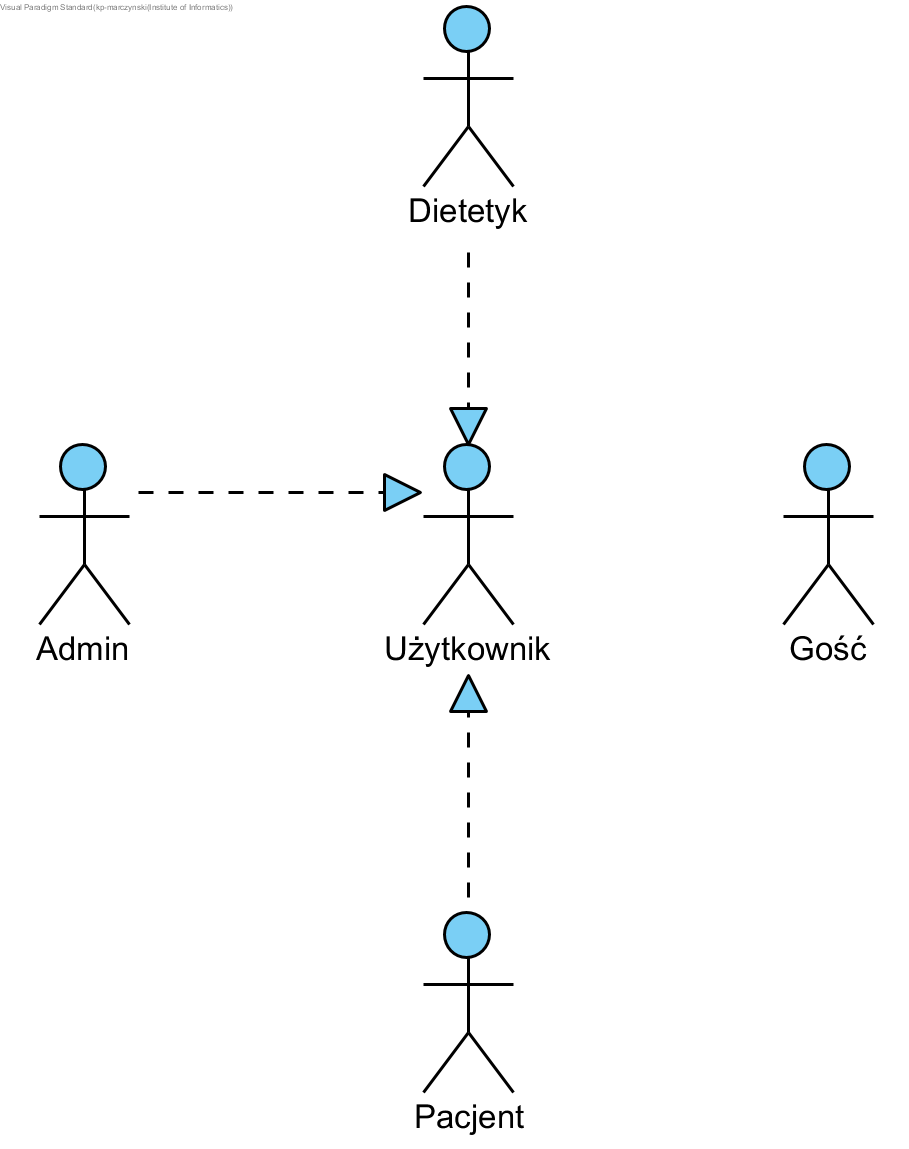
\includegraphics[scale=0.55]{../uml/use_case_diagrams/users.png}
        \caption{Użytkownicy - diagram przypadków użycia (opr.wł).}\label{rysunek:use-case-diagram-users}
    \end{figure}
\end{minipage}

\begin{minipage}{\textwidth}
    \begin{figure}[H]
        \centering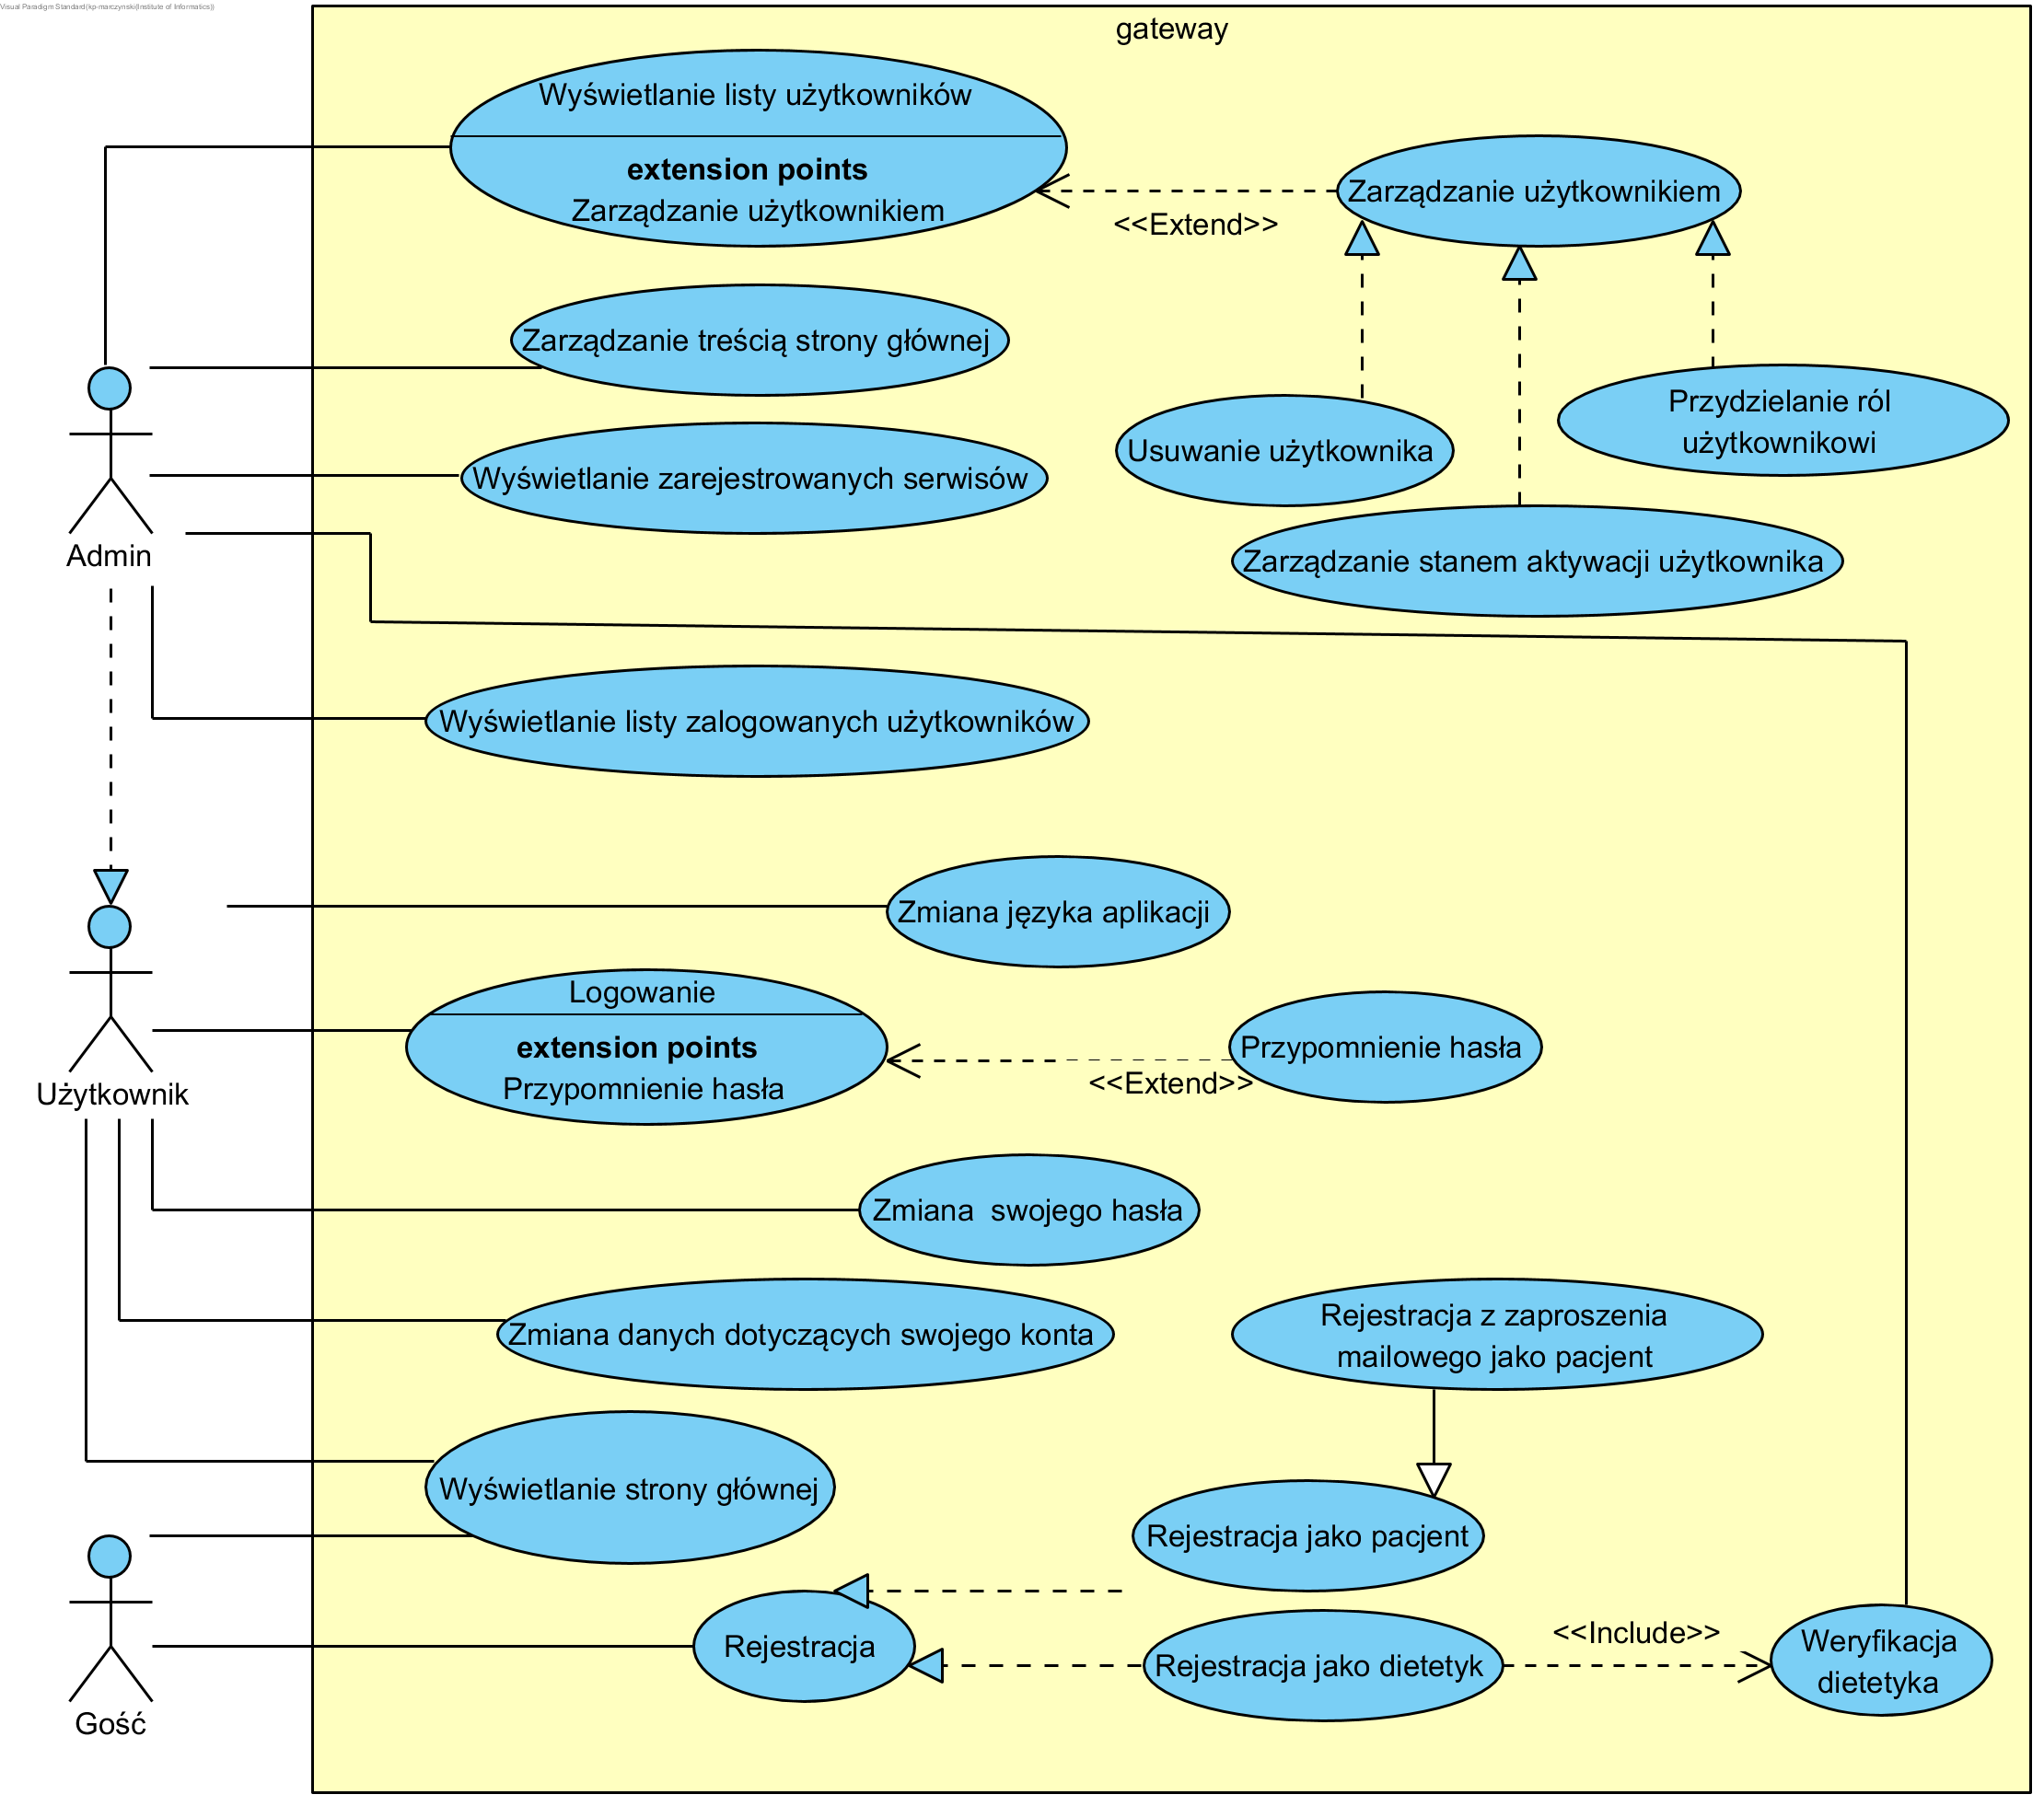
\includegraphics[scale=0.55]{../uml/use_case_diagrams/gateway.png}
        \caption{Gateway - diagram przypadków użycia (opr.wł).}\label{rysunek:use-case-diagram-gateway}
    \end{figure}
\end{minipage}

\begin{minipage}{\textwidth}
    \begin{figure}[H]
        \centering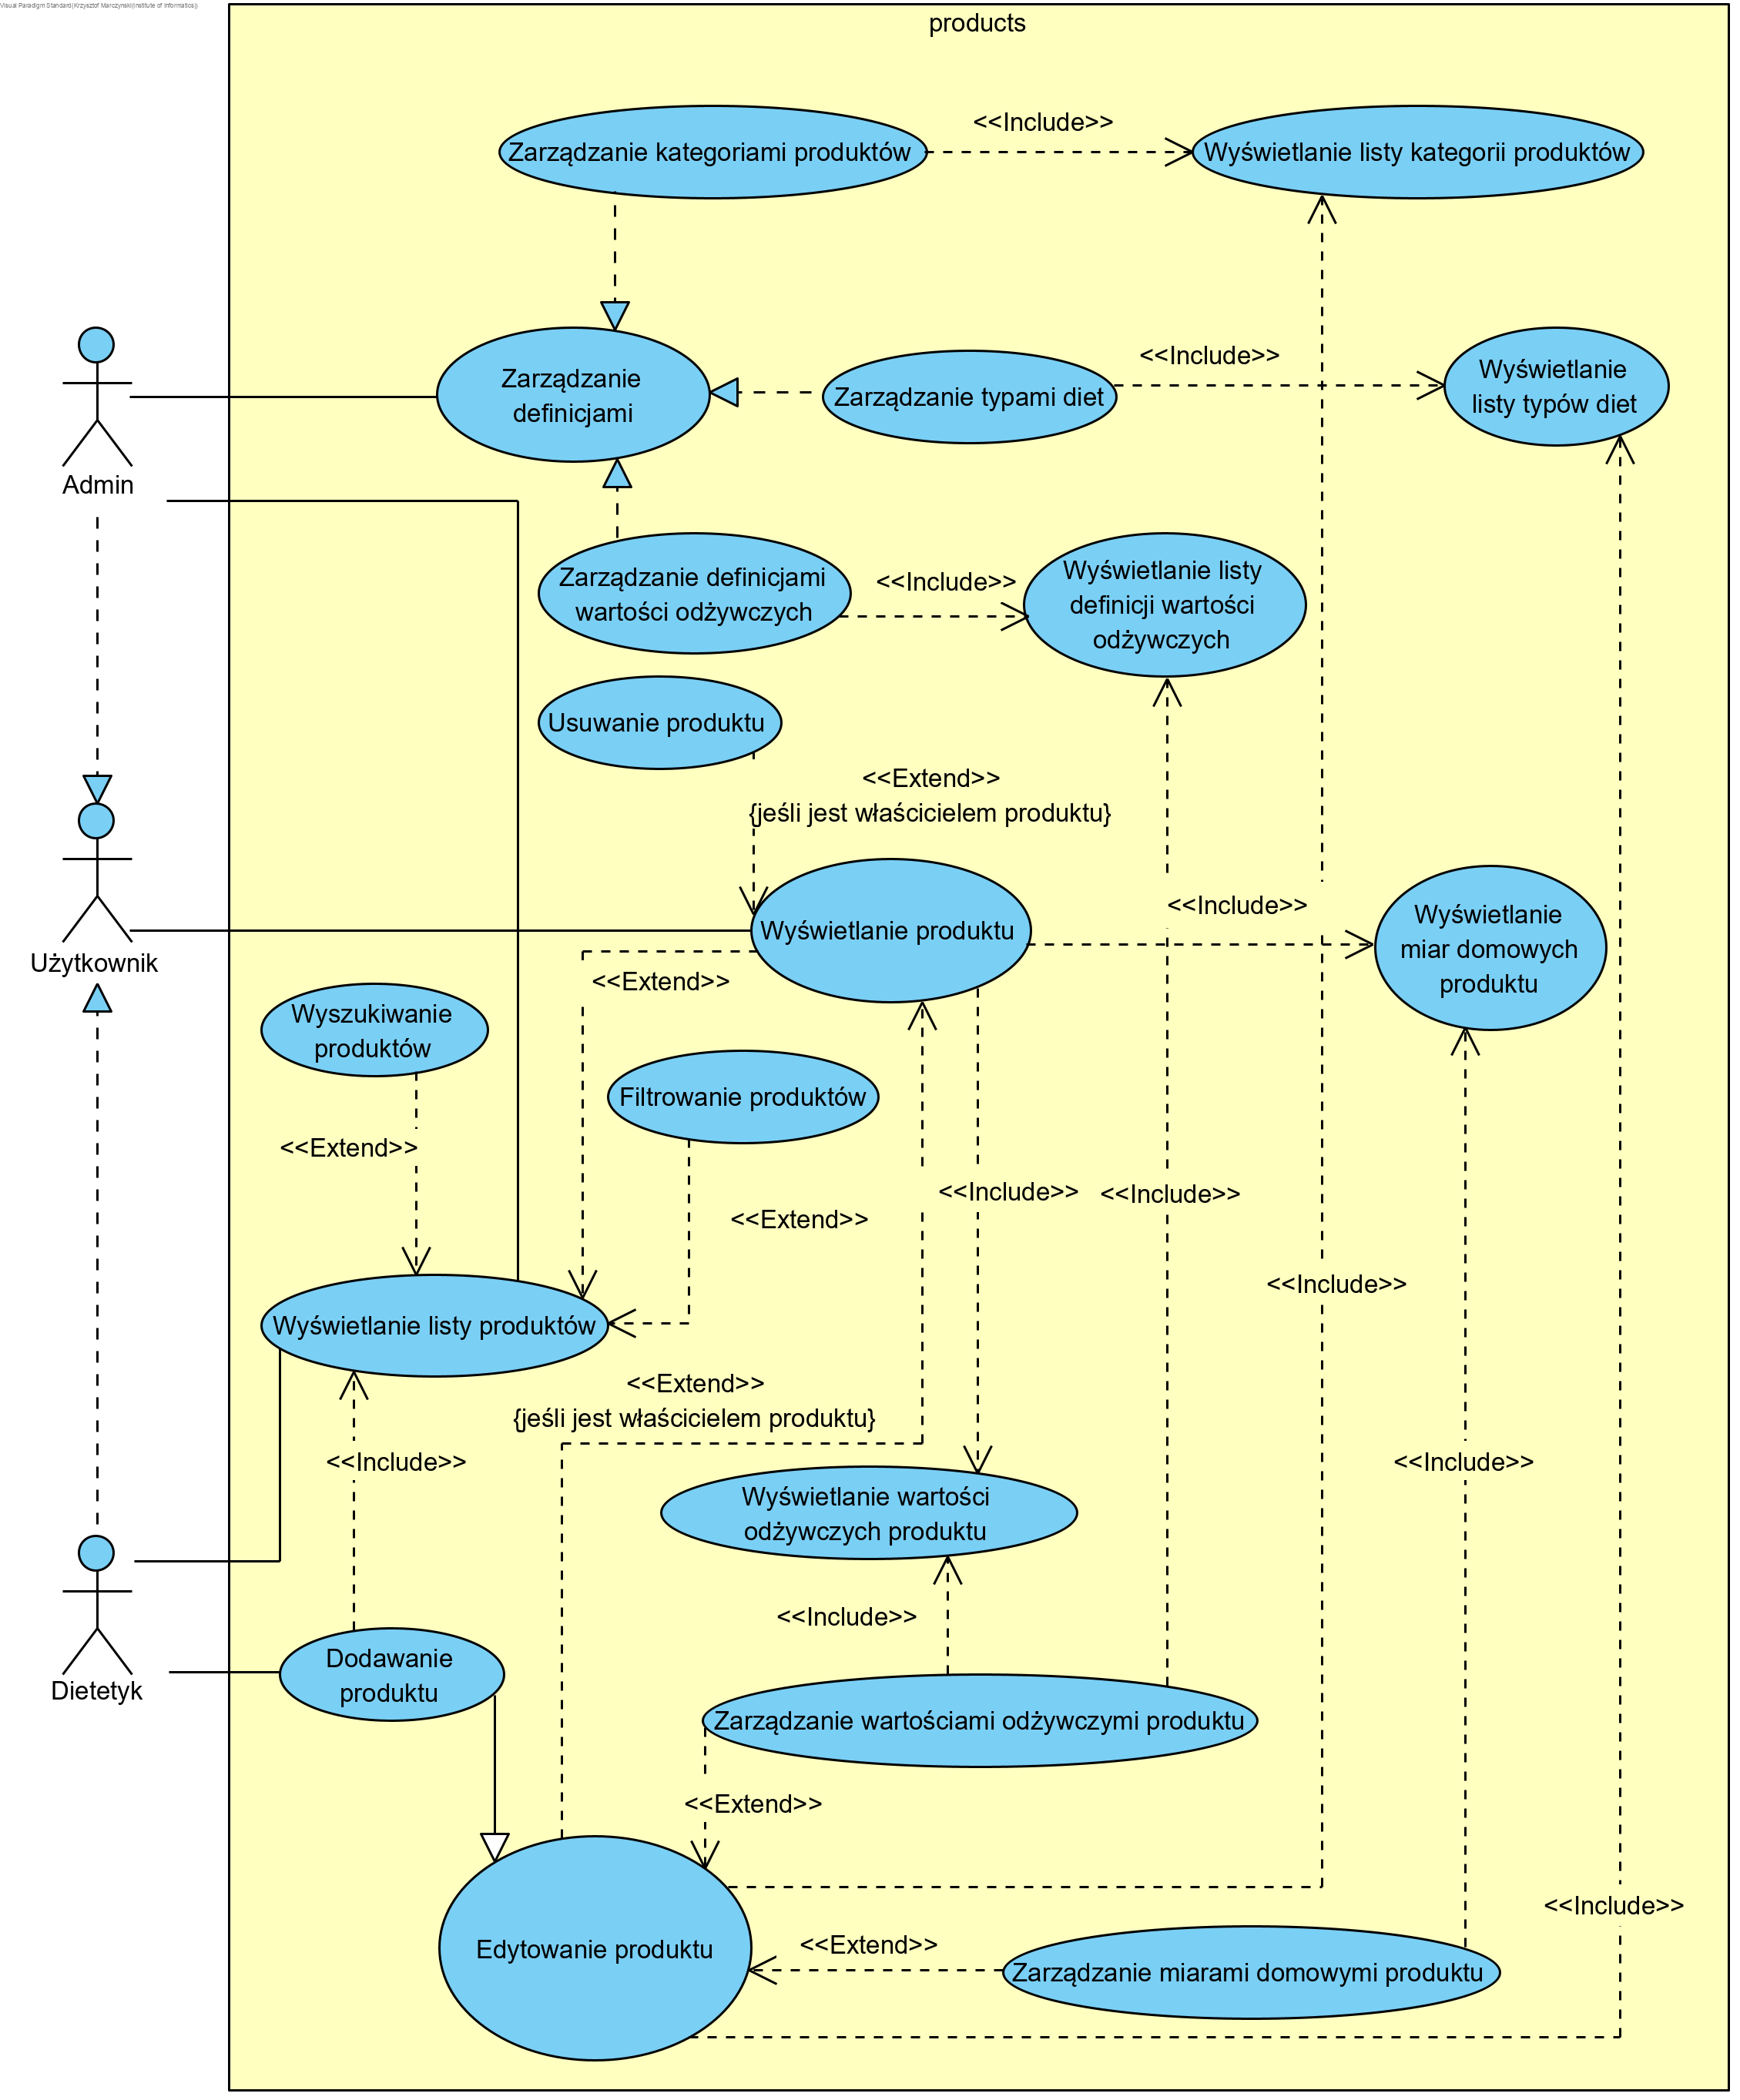
\includegraphics[scale=0.55]{../uml/use_case_diagrams/products.png}
        \caption{Produkty - diagram przypadków użycia (opr.wł).}\label{rysunek:use-case-diagram-products}
    \end{figure}
\end{minipage}

\begin{minipage}{\textwidth}
    \begin{figure}[H]
        \centering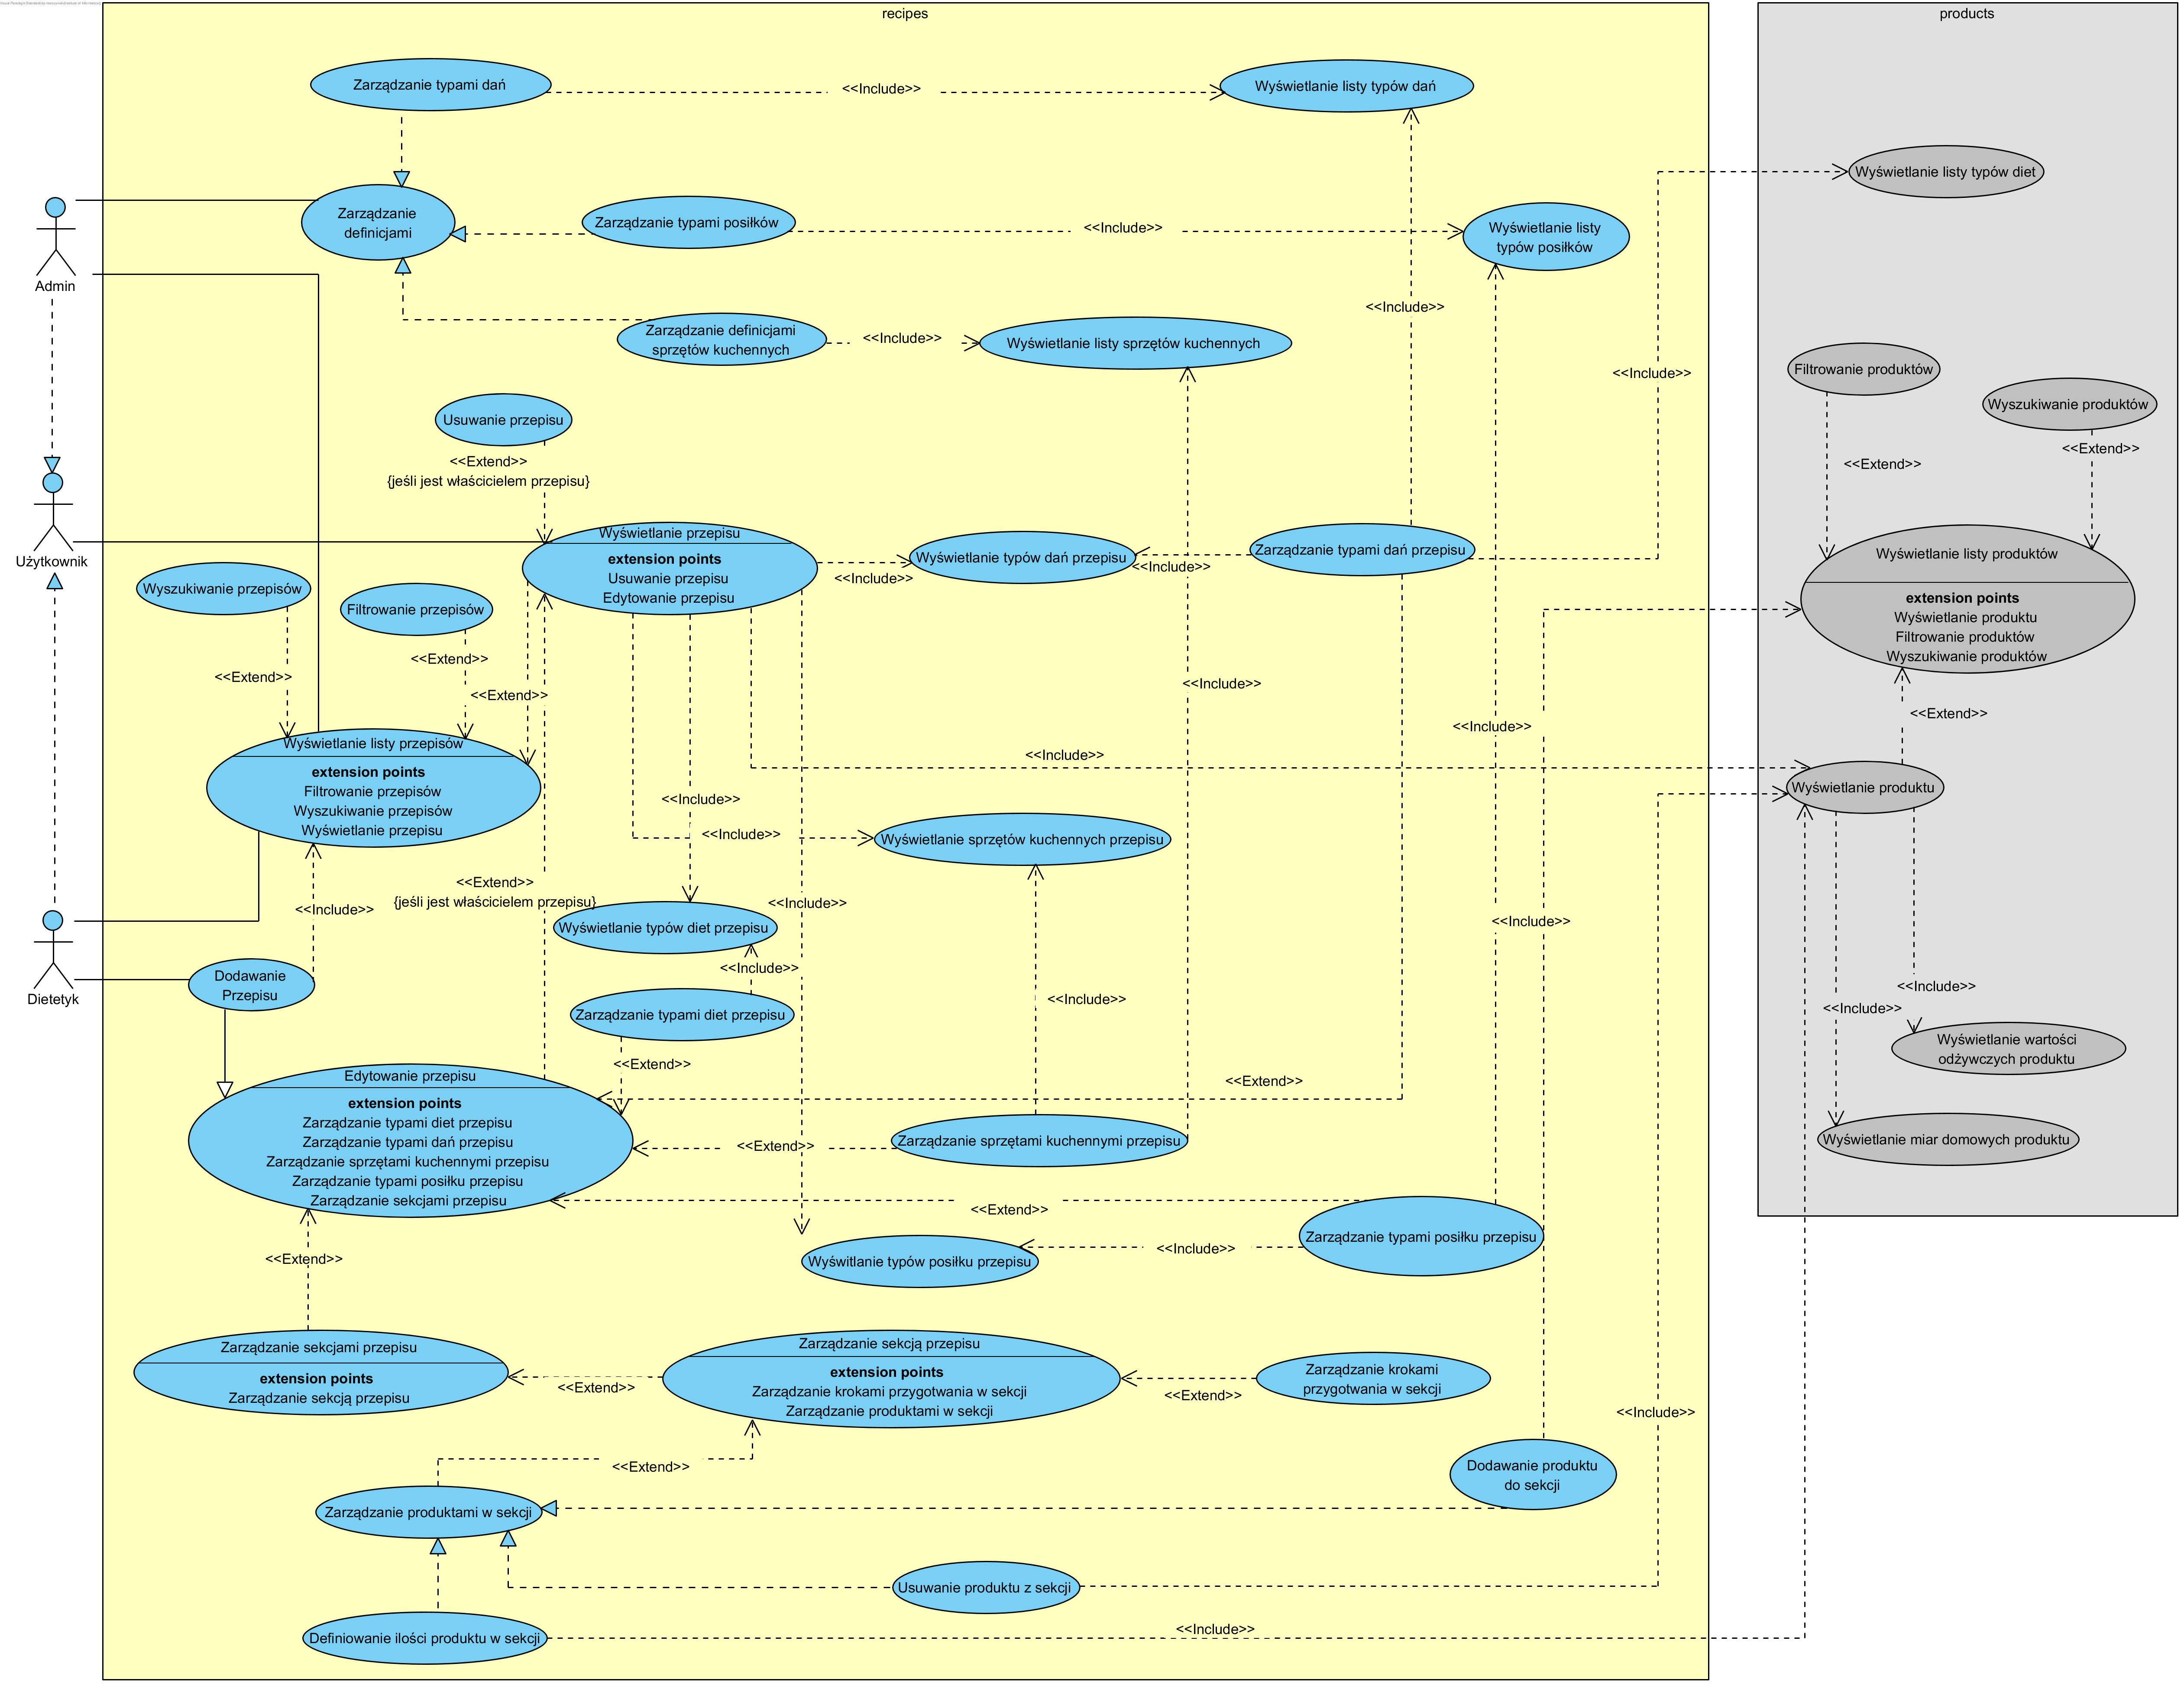
\includegraphics[scale=0.55]{../uml/use_case_diagrams/recipes.png}
        \caption{Przepisy - diagram przypadków użycia (opr.wł).}\label{rysunek:use-case-diagram-recipes}
    \end{figure}
\end{minipage}

\begin{minipage}{\textwidth}
    \begin{figure}[H]
        \centering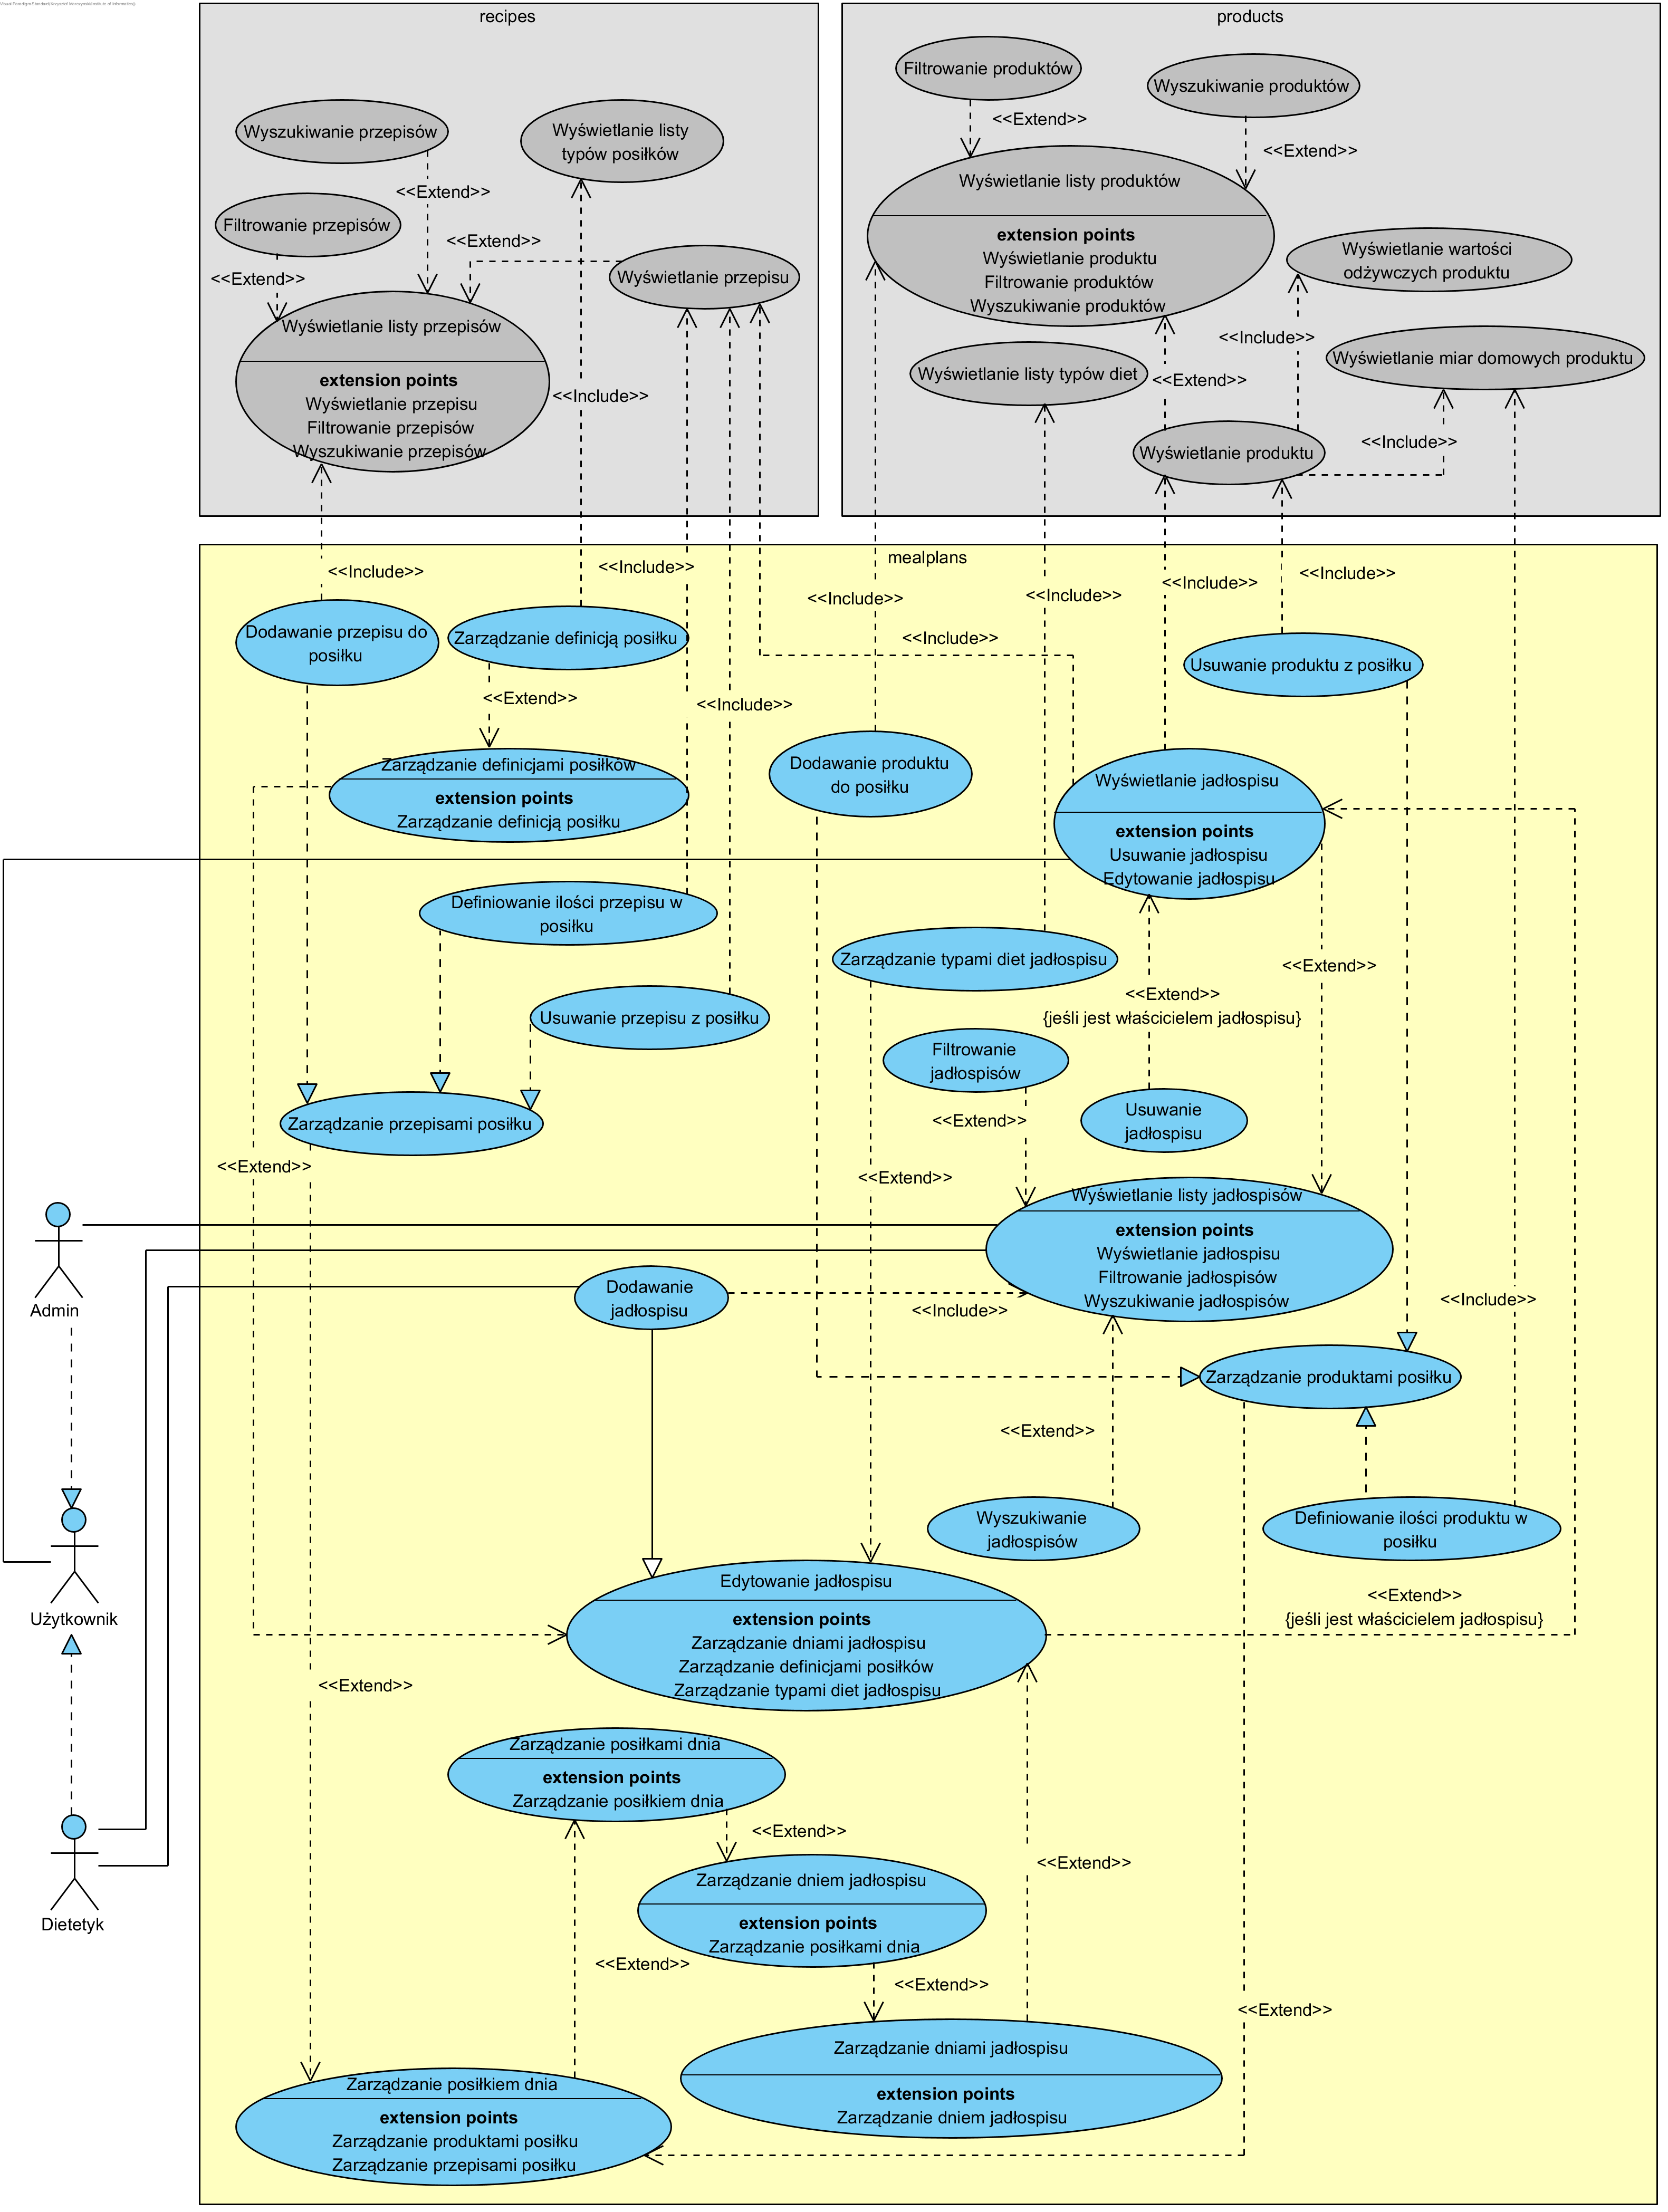
\includegraphics[scale=0.55]{../uml/use_case_diagrams/mealplans.png}
        \caption{Jadłospisy - diagram przypadków użycia (opr.wł).}\label{rysunek:use-case-diagram-mealplans}
    \end{figure}
\end{minipage}

\begin{minipage}{\textwidth}
    \begin{figure}[H]
        \centering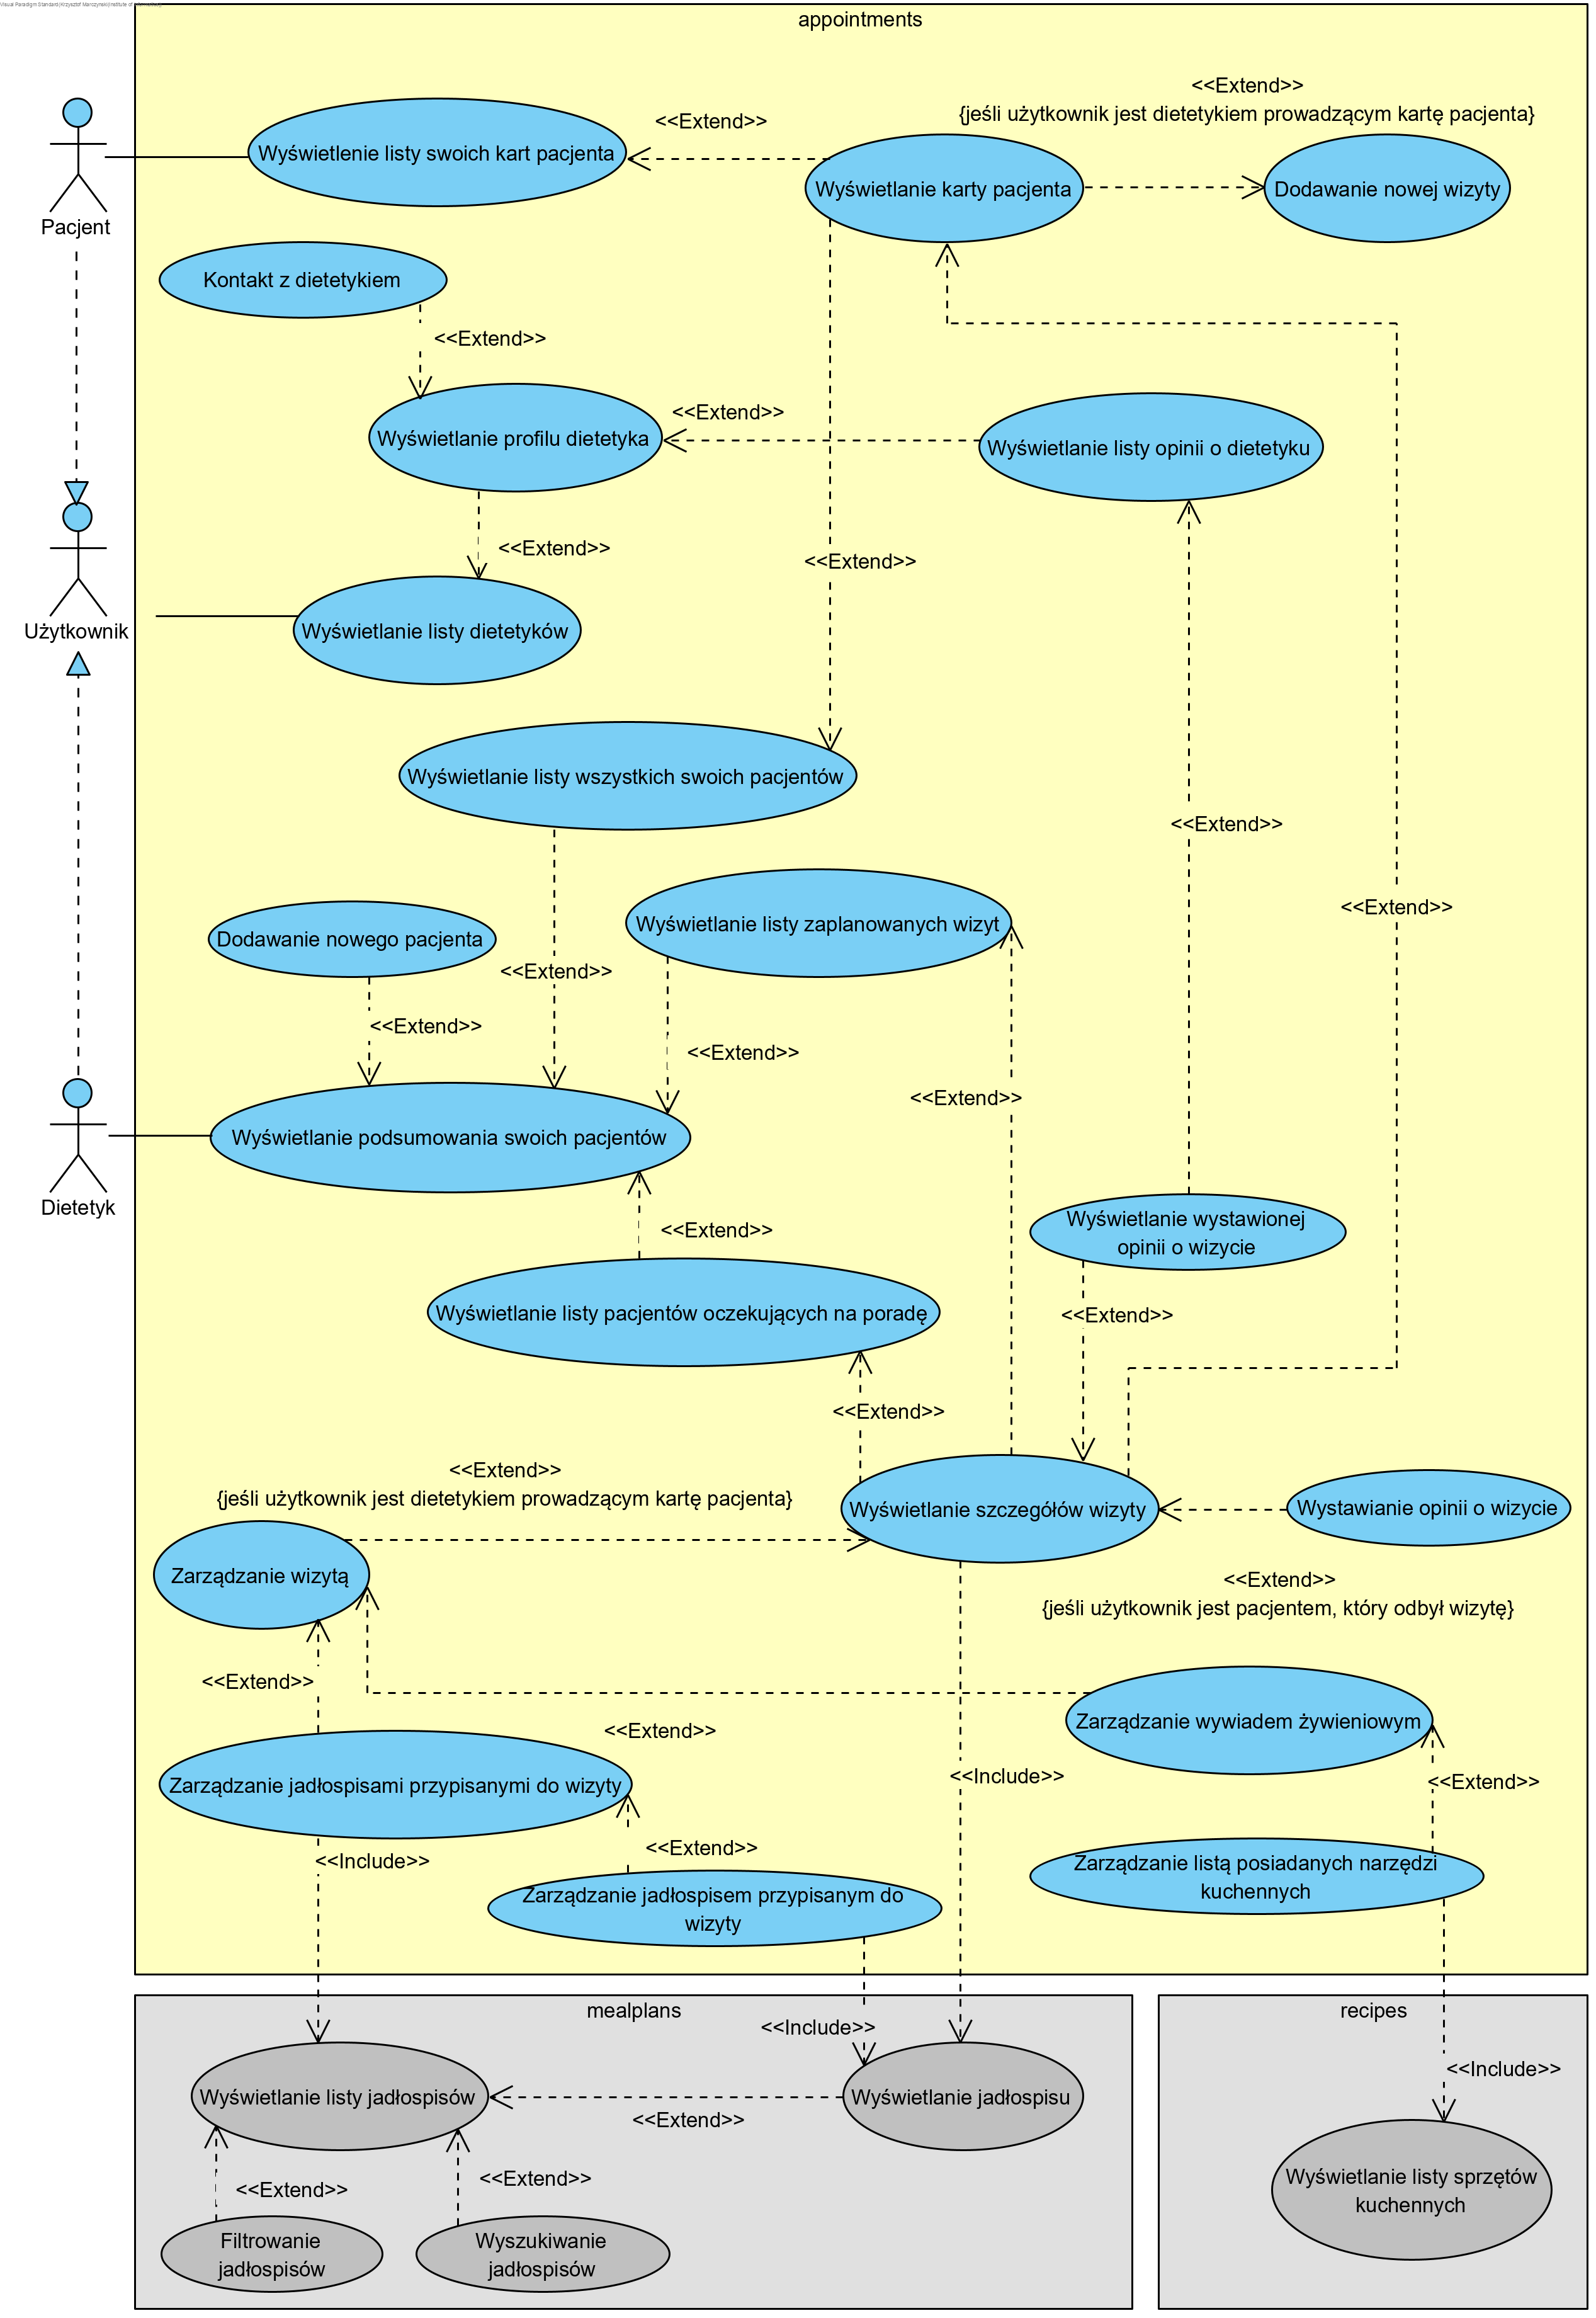
\includegraphics[scale=0.55]{../uml/use_case_diagrams/appointments.png}
        \caption{Wizyty - diagram przypadków użycia (opr.wł).}\label{rysunek:use-case-diagram-appointments}
    \end{figure}
\end{minipage}

\section{Prototyp interfejsu}\label{sec:mockups}
\todo{Podpisy i opisy mockupów}

\begin{minipage}{\textwidth}
    \begin{figure}[H]
        \centering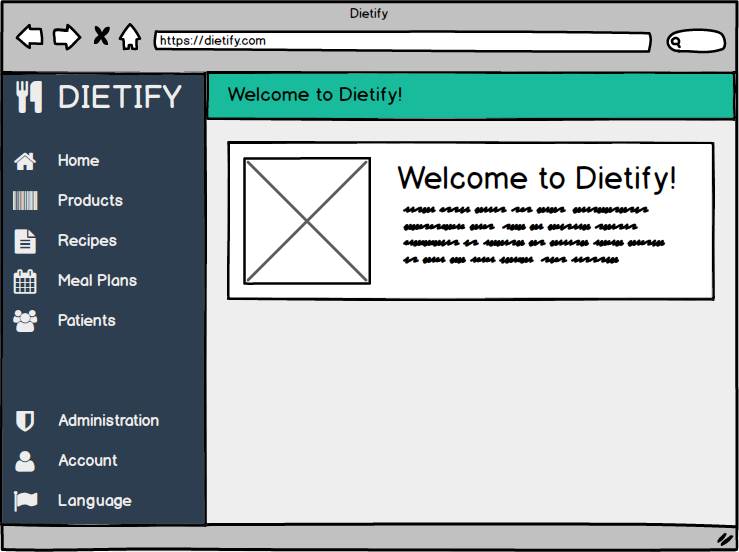
\includegraphics[scale=0.55]{../mockup/0home.png}
        \caption{Prototyp interfejsu - 0home (opr.wł)}\label{rysunek:0home}
    \end{figure}
\end{minipage}
\begin{minipage}{\textwidth}
    \begin{figure}[H]
        \centering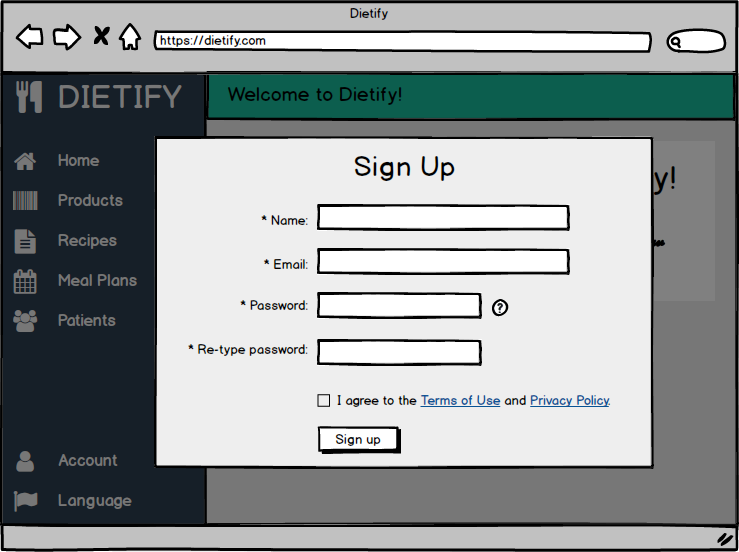
\includegraphics[scale=0.55]{../mockup/0home_1sign-up.png}
        \caption{Prototyp interfejsu - 0home:1sign-up (opr.wł)}\label{rysunek:0home_1sign-up}
    \end{figure}
\end{minipage}
\begin{minipage}{\textwidth}
    \begin{figure}[H]
        \centering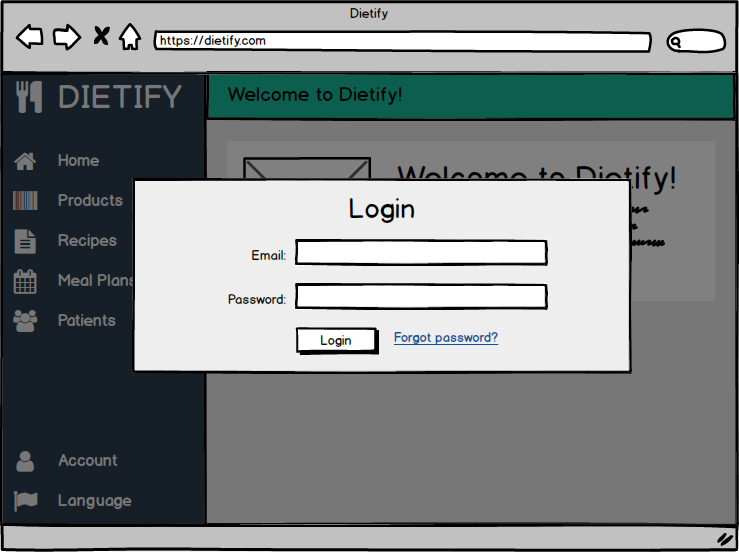
\includegraphics[scale=0.55]{../mockup/0home_2login.png}
        \caption{Prototyp interfejsu - 0home:2login (opr.wł)}\label{rysunek:0home_2login}
    \end{figure}
\end{minipage}
\begin{minipage}{\textwidth}
    \begin{figure}[H]
        \centering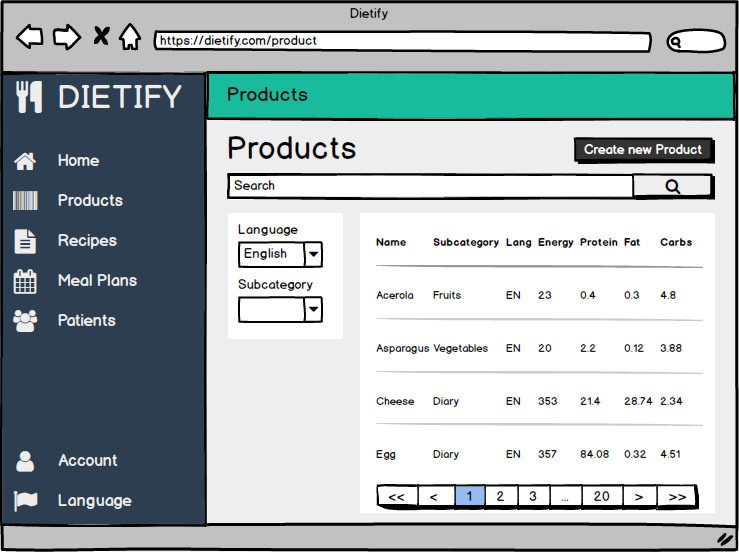
\includegraphics[scale=0.55]{../mockup/1products.png}
        \caption{Prototyp interfejsu - 1products (opr.wł)}\label{rysunek:1products}
    \end{figure}
\end{minipage}
\begin{minipage}{\textwidth}
    \begin{figure}[H]
        \centering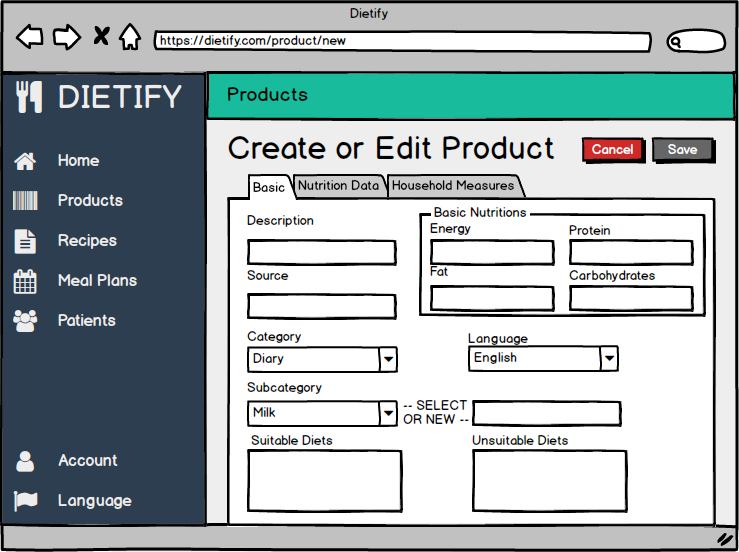
\includegraphics[scale=0.55]{../mockup/1products_1new.png}
        \caption{Prototyp interfejsu - 1products:1new (opr.wł)}\label{rysunek:1products_1new}
    \end{figure}
\end{minipage}
\begin{minipage}{\textwidth}
    \begin{figure}[H]
        \centering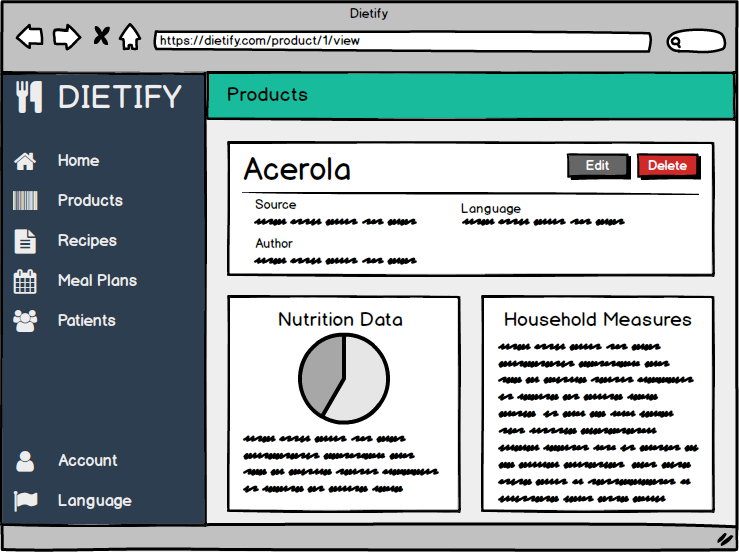
\includegraphics[scale=0.55]{../mockup/1products_2details.png}
        \caption{Prototyp interfejsu - 1products:2details (opr.wł)}\label{rysunek:1products_2details}
    \end{figure}
\end{minipage}
\begin{minipage}{\textwidth}
    \begin{figure}[H]
        \centering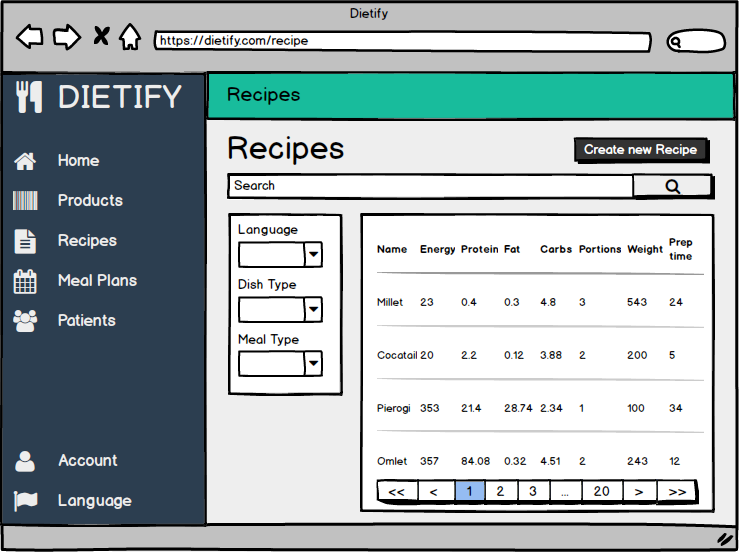
\includegraphics[scale=0.55]{../mockup/2recipes.png}
        \caption{Prototyp interfejsu - 2recipes (opr.wł)}\label{rysunek:2recipes}
    \end{figure}
\end{minipage}
\begin{minipage}{\textwidth}
    \begin{figure}[H]
        \centering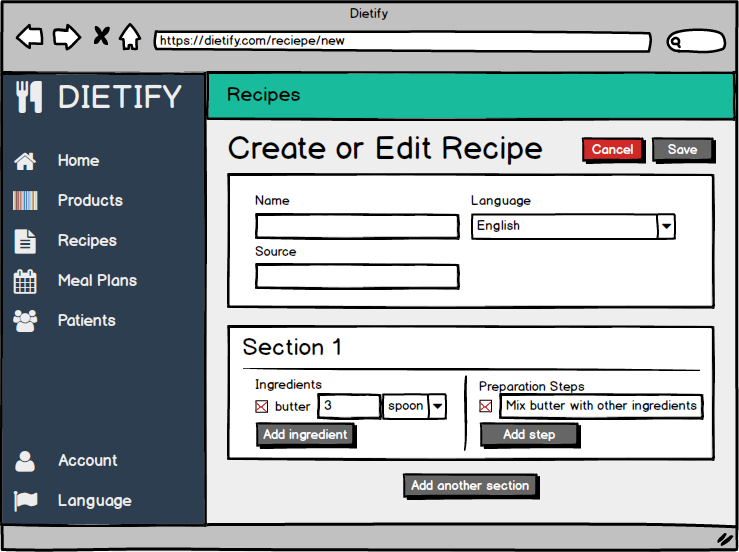
\includegraphics[scale=0.55]{../mockup/2recipes_1new.png}
        \caption{Prototyp interfejsu - 2recipes:1new (opr.wł)}\label{rysunek:2recipes_1new}
    \end{figure}
\end{minipage}
\begin{minipage}{\textwidth}
    \begin{figure}[H]
        \centering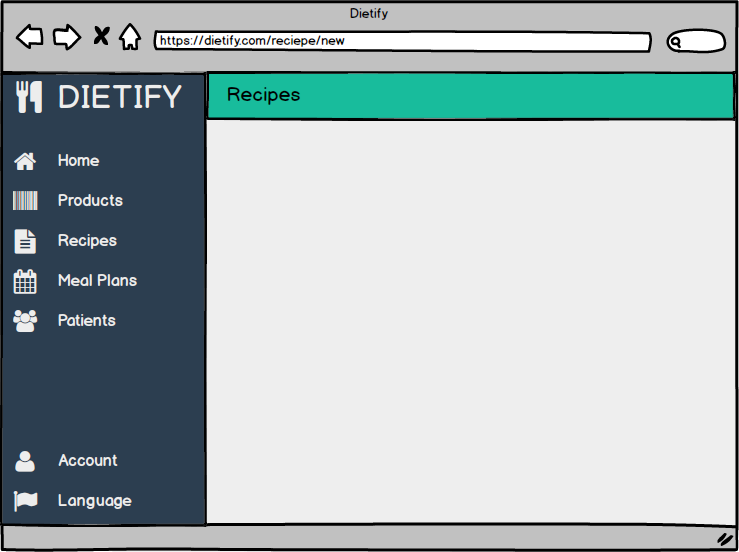
\includegraphics[scale=0.55]{../mockup/2recipes_1new_1add-product.png}
        \caption{Prototyp interfejsu - 2recipes:1new:1add-product (opr.wł)}\label{rysunek:2recipes_1new_1add-product}
    \end{figure}
\end{minipage}
\begin{minipage}{\textwidth}
    \begin{figure}[H]
        \centering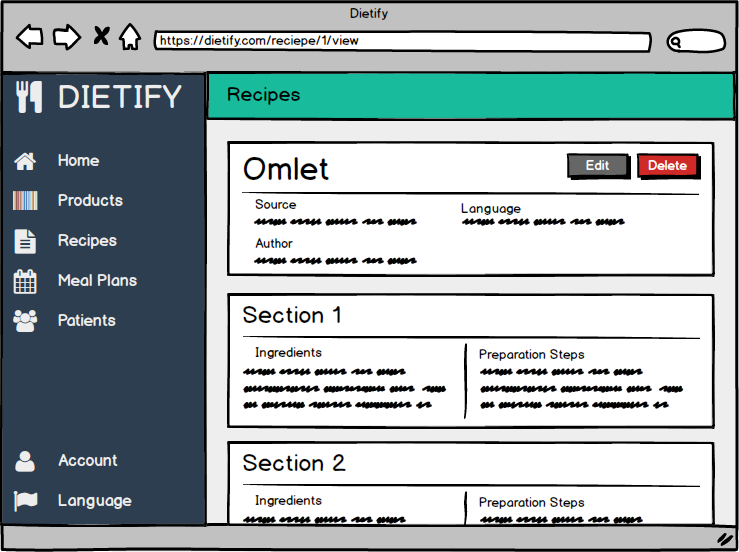
\includegraphics[scale=0.55]{../mockup/2recipes_2details.png}
        \caption{Prototyp interfejsu - 2recipes:2details (opr.wł)}\label{rysunek:2recipes_2details}
    \end{figure}
\end{minipage}
\begin{minipage}{\textwidth}
    \begin{figure}[H]
        \centering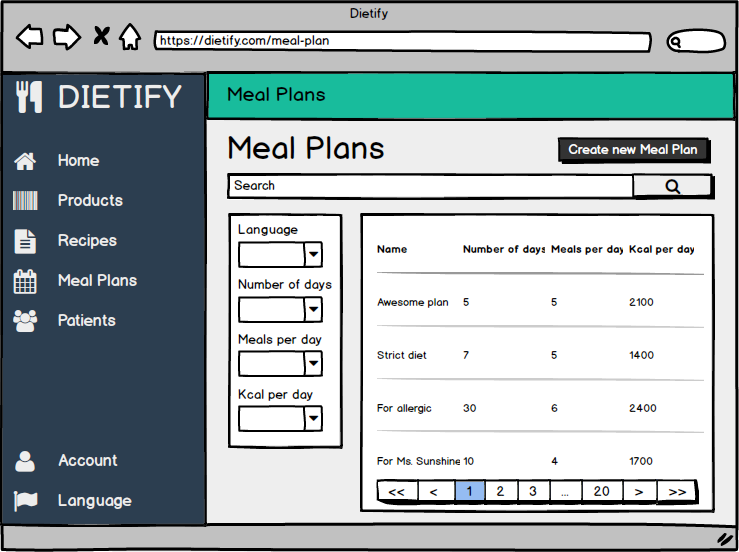
\includegraphics[scale=0.55]{../mockup/3mealplans.png}
        \caption{Prototyp interfejsu - 3mealplans (opr.wł)}\label{rysunek:3mealplans}
    \end{figure}
\end{minipage}
\begin{minipage}{\textwidth}
    \begin{figure}[H]
        \centering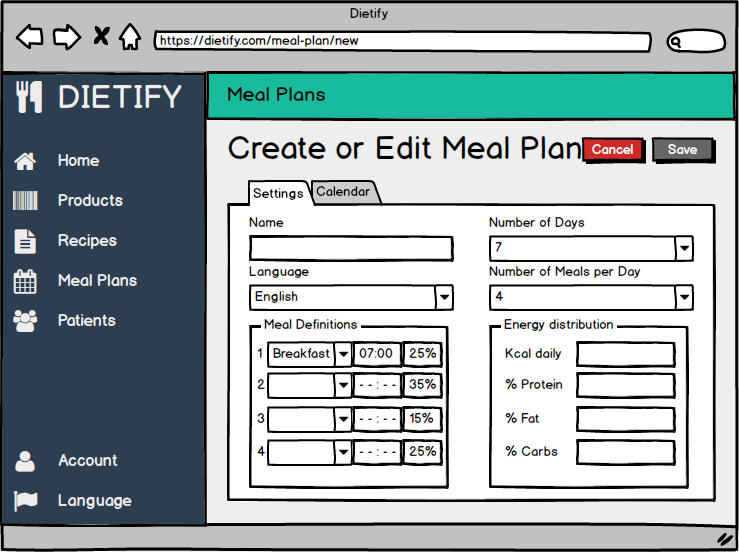
\includegraphics[scale=0.55]{../mockup/3mealplans_1new_1settings.png}
        \caption{Prototyp interfejsu - 3mealplans:1new:1settings (opr.wł)}\label{rysunek:3mealplans_1new_1settings}
    \end{figure}
\end{minipage}
\begin{minipage}{\textwidth}
    \begin{figure}[H]
        \centering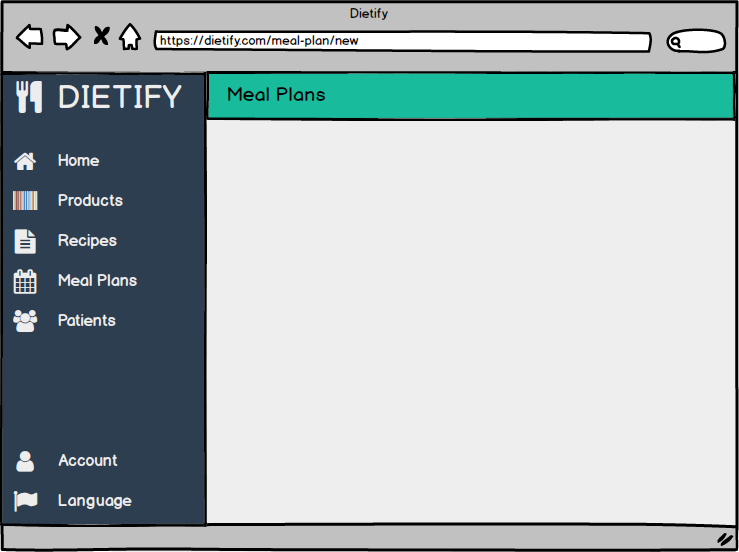
\includegraphics[scale=0.55]{../mockup/3mealplans_1new_2calendar.png}
        \caption{Prototyp interfejsu - 3mealplans:1new:2calendar (opr.wł)}\label{rysunek:3mealplans_1new_2calendar}
    \end{figure}
\end{minipage}
\begin{minipage}{\textwidth}
    \begin{figure}[H]
        \centering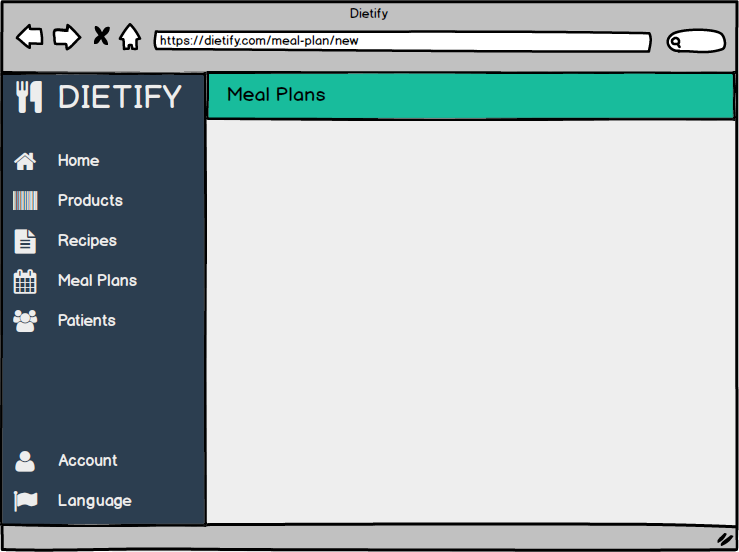
\includegraphics[scale=0.55]{../mockup/3mealplans_1new_2calendar_1meal.png}
        \caption{Prototyp interfejsu - 3mealplans:1new:2calendar:1meal (opr.wł)}\label{rysunek:3mealplans_1new_2calendar_1meal}
    \end{figure}
\end{minipage}
\begin{minipage}{\textwidth}
    \begin{figure}[H]
        \centering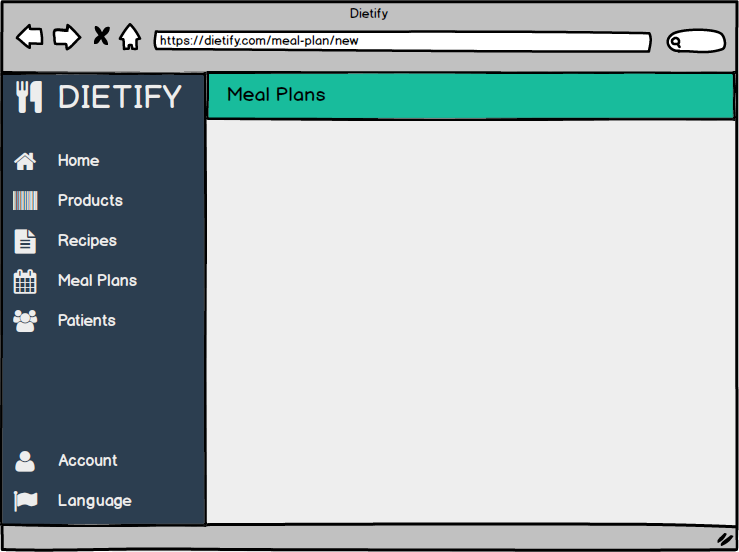
\includegraphics[scale=0.55]{../mockup/3mealplans_1new_2calendar_2add-product.png}
        \caption{Prototyp interfejsu - 3mealplans:1new:2calendar:2add-product (opr.wł)}\label{rysunek:3mealplans_1new_2calendar_2add-product}
    \end{figure}
\end{minipage}
\begin{minipage}{\textwidth}
    \begin{figure}[H]
        \centering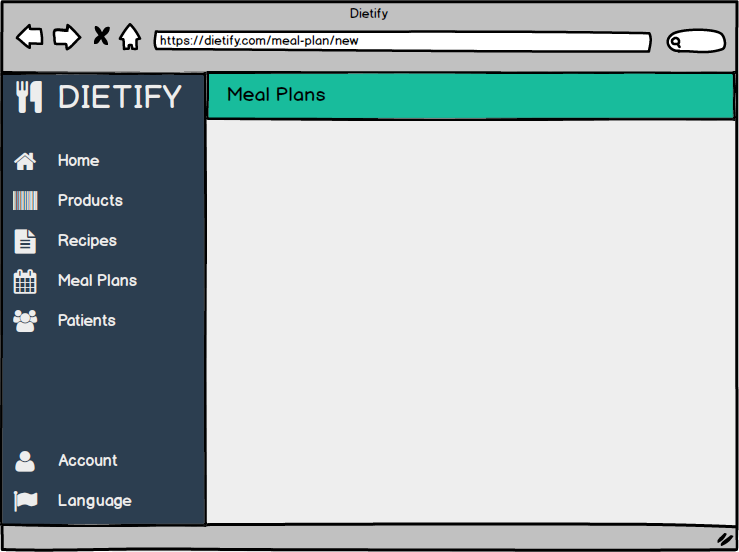
\includegraphics[scale=0.55]{../mockup/3mealplans_1new_2calendar_3add-recipe.png}
        \caption{Prototyp interfejsu - 3mealplans:1new:2calendar:3add-recipe (opr.wł)}\label{rysunek:3mealplans_1new_2calendar_3add-recipe}
    \end{figure}
\end{minipage}
\begin{minipage}{\textwidth}
    \begin{figure}[H]
        \centering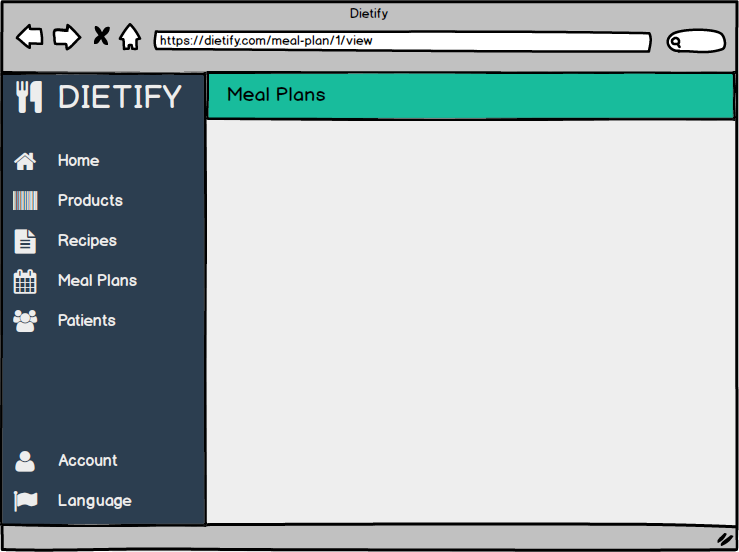
\includegraphics[scale=0.55]{../mockup/3mealplans_2details_1settings.png}
        \caption{Prototyp interfejsu - 3mealplans:2details:1settings (opr.wł)}\label{rysunek:3mealplans_2details_1settings}
    \end{figure}
\end{minipage}
\begin{minipage}{\textwidth}
    \begin{figure}[H]
        \centering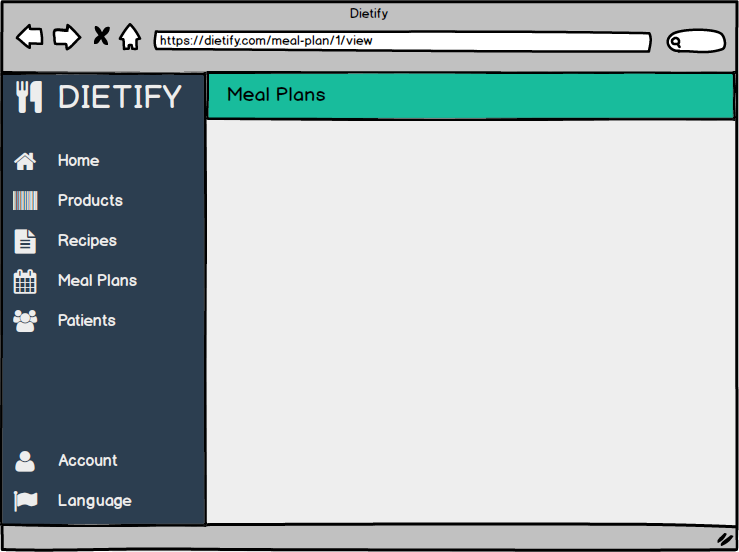
\includegraphics[scale=0.55]{../mockup/3mealplans_2details_2calendar.png}
        \caption{Prototyp interfejsu - 3mealplans:2details:2calendar (opr.wł)}\label{rysunek:3mealplans_2details_2calendar}
    \end{figure}
\end{minipage}
\begin{minipage}{\textwidth}
    \begin{figure}[H]
        \centering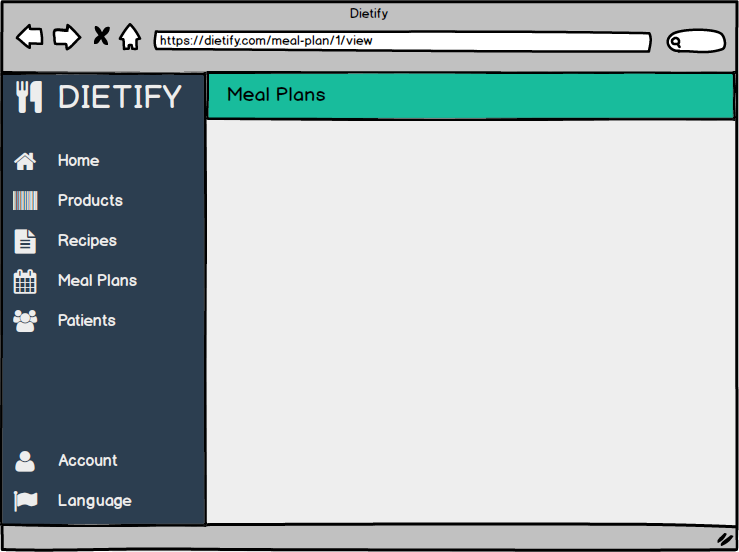
\includegraphics[scale=0.55]{../mockup/3mealplans_2details_2calendar_1meal.png}
        \caption{Prototyp interfejsu - 3mealplans:2details:2calendar:1meal (opr.wł)}\label{rysunek:3mealplans_2details_2calendar_1meal}
    \end{figure}
\end{minipage}
\begin{minipage}{\textwidth}
    \begin{figure}[H]
        \centering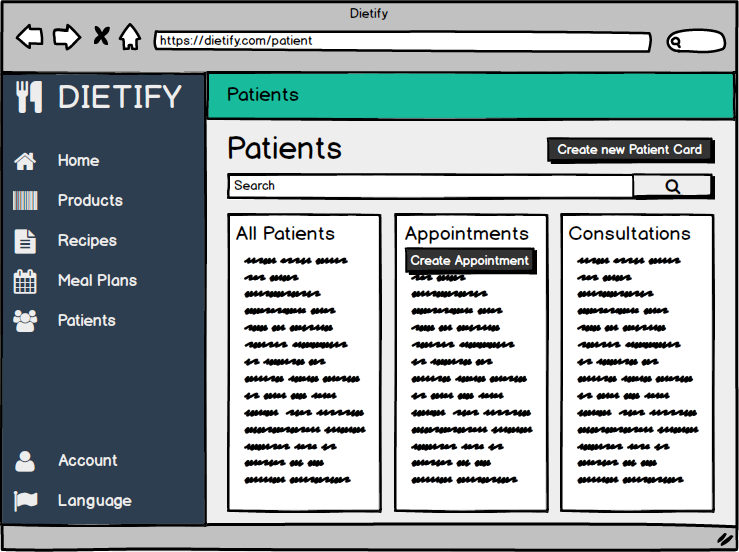
\includegraphics[scale=0.55]{../mockup/4appointments.png}
        \caption{Prototyp interfejsu - 4appointments (opr.wł)}\label{rysunek:4appointments}
    \end{figure}
\end{minipage}
\begin{minipage}{\textwidth}
    \begin{figure}[H]
        \centering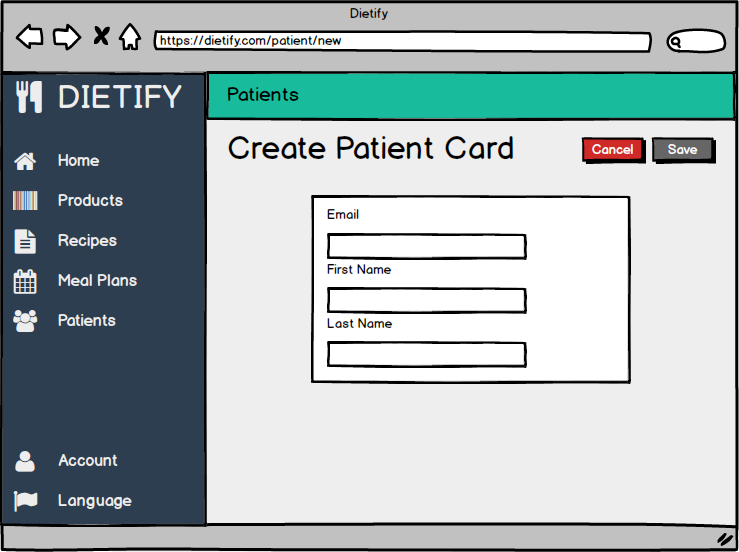
\includegraphics[scale=0.55]{../mockup/4appointments_1new-patient-card.png}
        \caption{Prototyp interfejsu - 4appointments:1new-patient-card (opr.wł)}\label{rysunek:4appointments_1new-patient-card}
    \end{figure}
\end{minipage}
\begin{minipage}{\textwidth}
    \begin{figure}[H]
        \centering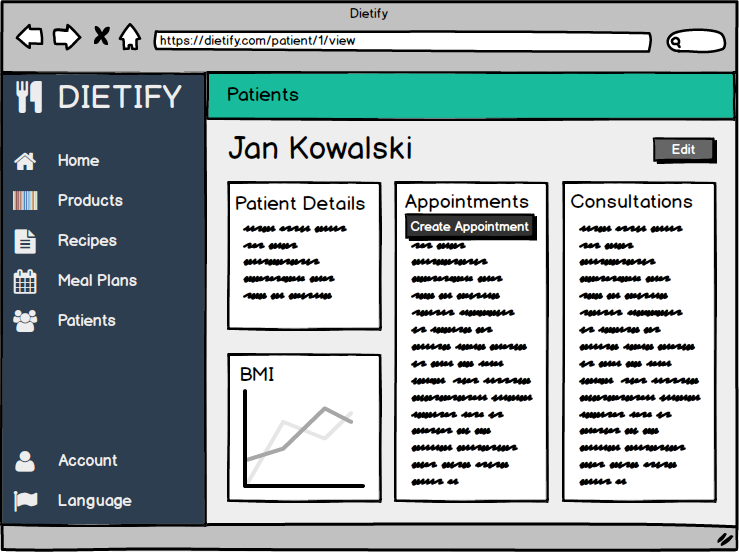
\includegraphics[scale=0.55]{../mockup/4appointments_2patient-card-details.png}
        \caption{Prototyp interfejsu - 4appointments:2patient-card-details (opr.wł)}\label{rysunek:4appointments_2patient-card-details}
    \end{figure}
\end{minipage}
\begin{minipage}{\textwidth}
    \begin{figure}[H]
        \centering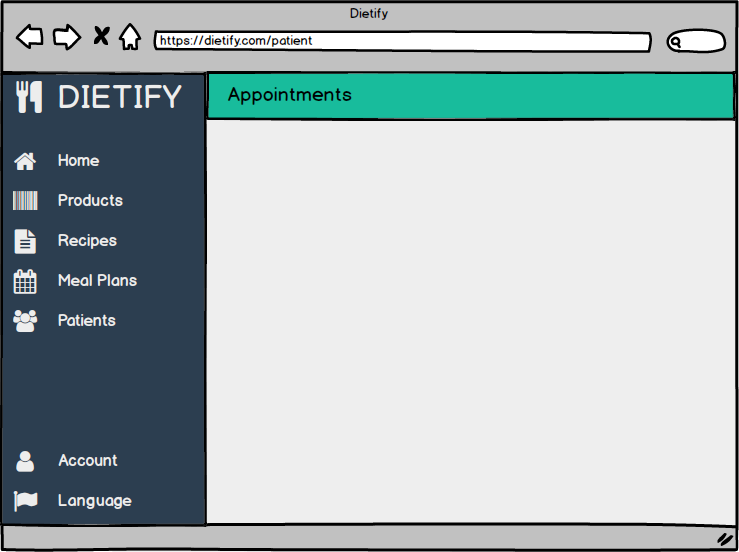
\includegraphics[scale=0.55]{../mockup/4appointments_3new-appointment.png}
        \caption{Prototyp interfejsu - 4appointments:3new-appointment (opr.wł)}\label{rysunek:4appointments_3new-appointment}
    \end{figure}
\end{minipage}
\begin{minipage}{\textwidth}
    \begin{figure}[H]
        \centering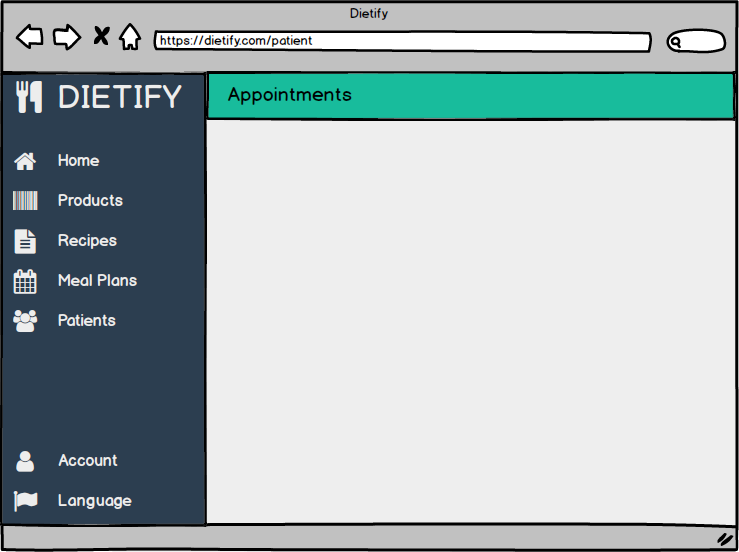
\includegraphics[scale=0.55]{../mockup/4appointments_4appointment-details.png}
        \caption{Prototyp interfejsu - 4appointments:4appointment-details (opr.wł)}\label{rysunek:4appointments_4appointment-details}
    \end{figure}
\end{minipage}
\begin{minipage}{\textwidth}
    \begin{figure}[H]
        \centering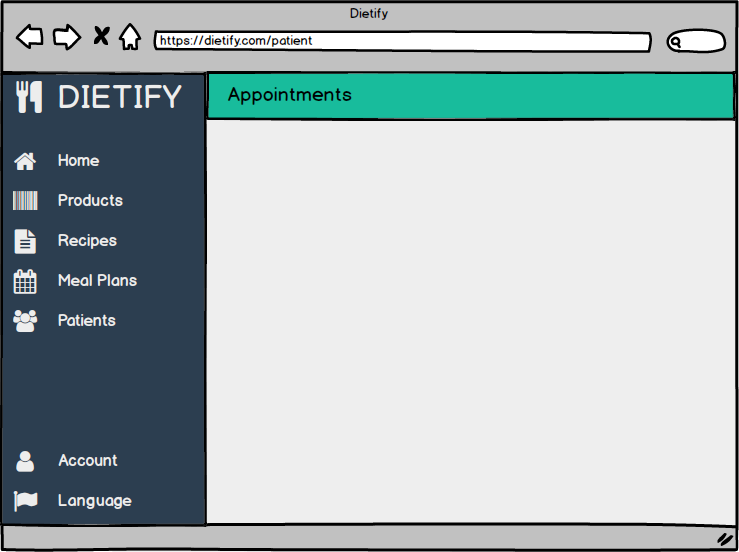
\includegraphics[scale=0.55]{../mockup/4appointments_4appointment-details_1nutritional-interview.png}
        \caption{Prototyp interfejsu - 4appointments:4appointment-details:1nutritional-interview (opr.wł)}\label{rysunek:4appointments_4appointment-details_1nutritional-interview}
    \end{figure}
\end{minipage}
\begin{minipage}{\textwidth}
    \begin{figure}[H]
        \centering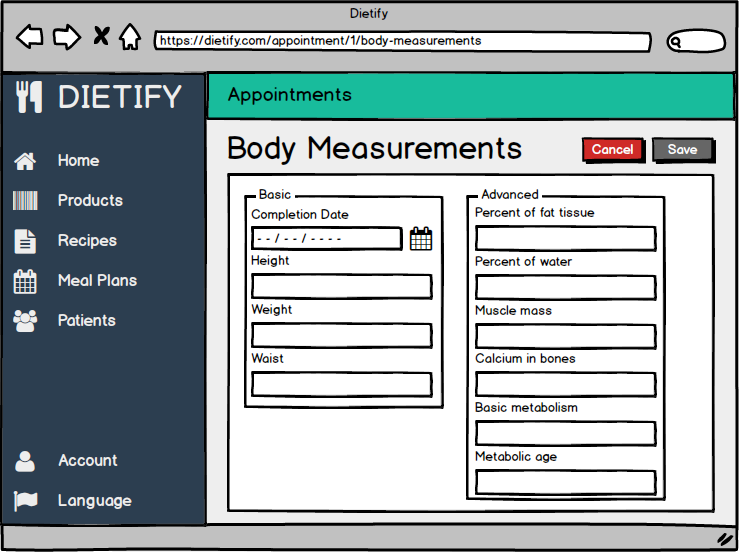
\includegraphics[scale=0.55]{../mockup/4appointments_4appointment-details_2body-measurement.png}
        \caption{Prototyp interfejsu - 4appointments:4appointment-details:2body-measurement (opr.wł)}\label{rysunek:4appointments_4appointment-details_2body-measurement}
    \end{figure}
\end{minipage}
\begin{minipage}{\textwidth}
    \begin{figure}[H]
        \centering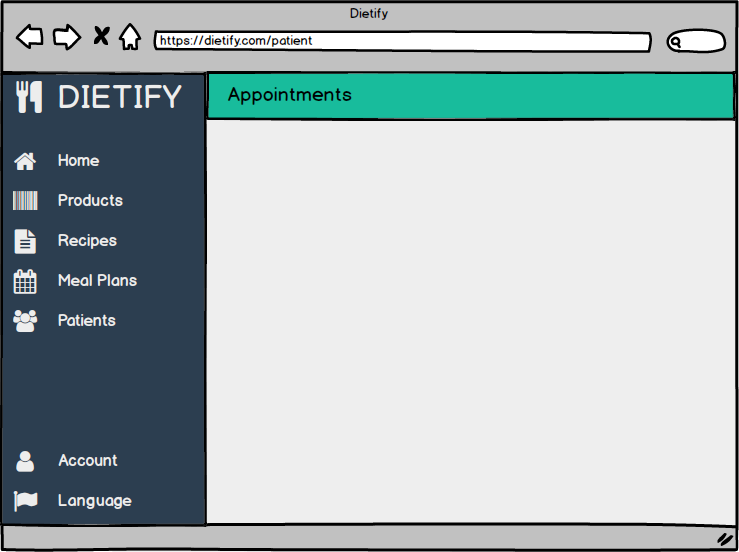
\includegraphics[scale=0.55]{../mockup/4appointments_4appointment-details_3mealplan.png}
        \caption{Prototyp interfejsu - 4appointments:4appointment-details:3mealplan (opr.wł)}\label{rysunek:4appointments_4appointment-details_3mealplan}
    \end{figure}
\end{minipage}
\begin{minipage}{\textwidth}
    \begin{figure}[H]
        \centering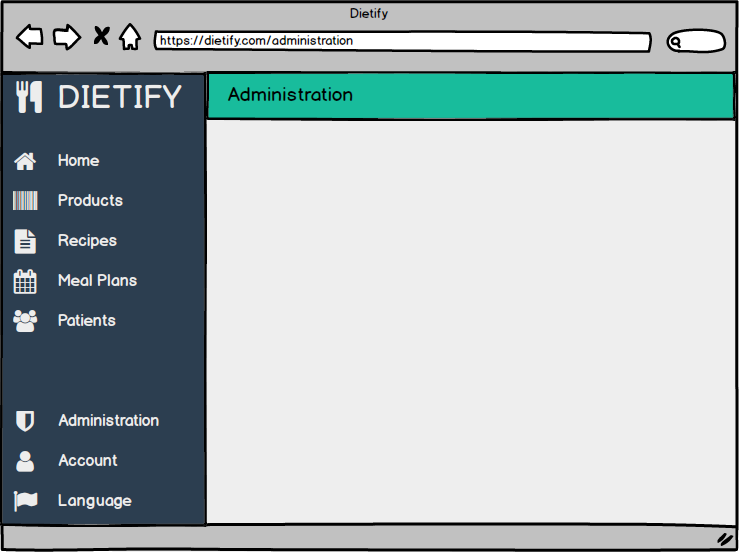
\includegraphics[scale=0.55]{../mockup/5administration.png}
        \caption{Prototyp interfejsu - 5administration (opr.wł)}\label{rysunek:5administration}
    \end{figure}
\end{minipage}

\section{Kategorie}\label{sec:categories}
\todo{uzupełnić kategorie}

\begin{enumerate}[label={\textbf{KAT/\protect\threedigits{\theenumi}}}, wide, labelwidth=!, labelindent=0pt, labelsep=0pt, series=reqs]
    \setlength\itemsep{1em}
    \req{User} \label{kat:User} (Użytkownik)

    \textbf{Opis}: Konto użytkownika aplikacji. Każdy zalogowany użytkownik musi mieć konto użytkownika
    \par
    \textbf{Atrybuty}:
    \begin{itemize}[series=atr, wide, align=left, leftmargin=5cm]
        \atr{id} \label{kat:User:id} - identyfikator
        \atr{login} \label{kat:User:login} - login użytkownika
        \atr{passwordHash} \label{kat:User:passwordHash} - reprezentacja hasła stworzona przez nałożenie na hasło funkcji skrótu
        \atr{firstName} \label{kat:User:firstName} - imię użytkownika
        \atr{lastName} \label{kat:User:lastName} - nazwisko użytkownika
        \atr{email} \label{kat:User:email} - adres email
        \atr{image} \label{kat:User:image} - zdjęcie profilowe użytkownika
        \atr{activated} \label{kat:User:activated} - flaga pokazująca czy konto użytkownika zostało aktywowane
        \atr{language} \label{kat:User:language} - język użytkownika w postaci kodu ISO 639-1
        \atr{activationKey} \label{kat:User:activationKey} - klucz wymagany podczas aktywacji konta użytkownika
        \atr{resetKey} \label{kat:User:resetKey} - klucz wymagany podczas resetowania hasła do konta użytkownika
        \atr{createdDate} \label{kat:User:createdDate} - data utworzenia konta
        \atr{resetDate} \label{kat:User:resetDate} - data ostatniego resetowania hasła do konta
        \atr{lastModifiedDate} \label{kat:User:lastModifiedDate} - data ostatniej modyfikacji konta
    \end{itemize}

    \req{Authority} \label{kat:Authority} (Rola)

    \textbf{Opis}: Rola użytkownika od której zależy zakres uprawnień użytkownika
    \par
    \textbf{Atrybuty}:
    \begin{itemize}[series=atr, wide, align=left, leftmargin=5cm]
        \atr{name} \label{kat:Authority:name} - nazwa roli
    \end{itemize}

    \req{UserExtraInfo} \label{kat:UserExtraInfo} (Dodatkowe Informacje Użytkownika)

    \textbf{Opis}: Dodatkowe informacje o użytkowniku
    \par
    \textbf{Atrybuty}:
    \begin{itemize}[series=atr, wide, align=left, leftmargin=5cm]
        \atr{id} \label{kat:UserExtraInfo:id} - identyfikator
        \atr{gender} \label{kat:UserExtraInfo:gender} - płeć
        \atr{dateOfBirth} \label{kat:UserExtraInfo:dateOfBirth} - data urodzenia
        \atr{phoneNumber} \label{kat:UserExtraInfo:phoneNumber} - numer telefonu, najlepiej w formacie (+00) 000-000-000
        \atr{streetAddress} \label{kat:UserExtraInfo:streetAddress} - adres zamieszkania
        \atr{postalCode} \label{kat:UserExtraInfo:postalCode} - kod pocztowy
        \atr{city} \label{kat:UserExtraInfo:city} - miasto
        \atr{country} \label{kat:UserExtraInfo:country} - państwo
        \atr{personalDescription} \label{kat:UserExtraInfo:personalDescription} - krótki opis osobisty. W przypadku dietyka może zawierać dodatkowe informacje o prowadzonej praktyce dietetycznej
    \end{itemize}

    \req{SiteContent} \label{kat:SiteContent} (Treść Strony)

    \textbf{Opis}: Treść strony definiowana przez administratora
    \par
    \textbf{Atrybuty}:
    \begin{itemize}[series=atr, wide, align=left, leftmargin=5cm]
        \atr{id} \label{kat:SiteContent:id} - identyfikator
        \atr{ordinalNumber} \label{kat:SiteContent:ordinalNumber} - numer porządkowy definiujący kolejność w jakim dane powinny być wyświetlane
        \atr{siteContentType} \label{kat:SiteContent:siteContentType} - typ treści strony
        \atr{title} \label{kat:SiteContent:title} - tytuł treści stron
        \atr{description} \label{kat:SiteContent:description} - opis treści strony
        \atr{image} \label{kat:SiteContent:image} - opcjonalny obrazek, który powinien zostać wyświetlony obok treści strony
    \end{itemize}

    \req{SiteContentTranslation} \label{kat:SiteContentTranslation} (Tłumaczenie Treści Strony)

    \textbf{Opis}: Tłumaczenie treści strony
    \par
    \textbf{Atrybuty}:
    \begin{itemize}[series=atr, wide, align=left, leftmargin=5cm]
        \atr{id} \label{kat:SiteContentTranslation:id} - identyfikator
        \atr{title} \label{kat:SiteContentTranslation:title} - tłumaczenie tytułu
        \atr{description} \label{kat:SiteContentTranslation:description} - tłumaczenie opisu
        \atr{language} \label{kat:SiteContentTranslation:language} - język tłumaczenia w postaci kodu ISO 639-1
    \end{itemize}

    \req{ContactInfo} \label{kat:ContactInfo} (Informacje Kontaktowe)

    \textbf{Opis}: Informacje kontaktowe witryny
    \par
    \textbf{Atrybuty}:
    \begin{itemize}[series=atr, wide, align=left, leftmargin=5cm]
        \atr{id} \label{kat:ContactInfo:id} - identyfikator
        \atr{contactInfoType} \label{kat:ContactInfo:contactInfoType} - typ informacji kontaktowej
        \atr{description} \label{kat:ContactInfo:description} - opis
    \end{itemize}

    \req{Pricing} \label{kat:Pricing} (Cennik)

    \textbf{Opis}: Pozycja cennika dostępu do usług oferowanych przez system
    \par
    \textbf{Atrybuty}:
    \begin{itemize}[series=atr, wide, align=left, leftmargin=5cm]
        \atr{id} \label{kat:Pricing:id} - identyfikator
        \atr{ordinalNumber} \label{kat:Pricing:ordinalNumber} - numer porządkowy warunkujący kolejność wyswietlania pozycji w cenniku
        \atr{title} \label{kat:Pricing:title} - nazwa pozycji cennika
        \atr{description} \label{kat:Pricing:description} - opis pozycji cennika
        \atr{price} \label{kat:Pricing:price} - cena
        \atr{currency} \label{kat:Pricing:currency} - waluta przedstawiona jako kod ISO 4217
    \end{itemize}

    \req{PricingTranslation} \label{kat:PricingTranslation} (Tłumaczenie Cennika)

    \textbf{Opis}: Tłumaczenie pozycji cennika
    \par
    \textbf{Atrybuty}:
    \begin{itemize}[series=atr, wide, align=left, leftmargin=5cm]
        \atr{id} \label{kat:PricingTranslation:id} - identyfikator
        \atr{title} \label{kat:PricingTranslation:title} - tłumaczenie nazwy
        \atr{description} \label{kat:PricingTranslation:description} - tłumaczenie opisu
        \atr{language} \label{kat:PricingTranslation:language} - język tłumaczenia w postaci kodu ISO 639-1
    \end{itemize}

    \req{Product} \label{kat:Product} (Produkt)

    \textbf{Opis}: \lipsum[1]
    \par
    \textbf{Atrybuty}:
    \begin{itemize}[series=atr, wide, align=left, leftmargin=5cm]
        \atr{id} \label{kat:Product:id}
        \atr{source} \label{kat:Product:source}
        \atr{isPublic} \label{kat:Product:isPublic}
        \atr{language} \label{kat:Product:language}
    \end{itemize}

    \req{ProductVersion} \label{kat:ProductVersion} (Wersja Produktu)

    \textbf{Opis}: \lipsum[1]
    \par
    \textbf{Atrybuty}:
    \begin{itemize}[series=atr, wide, align=left, leftmargin=5cm]
        \atr{id} \label{kat:ProductVersion:id}
        \atr{createdDate} \label{kat:ProductVersion:createdDate}
        \atr{description} \label{kat:ProductVersion:description}
    \end{itemize}

    \req{ProductBasicNutritionData} \label{kat:ProductBasicNutritionData} (Podstawowe Składniki Odżywcze Produktu)

    \textbf{Opis}: \lipsum[1]
    \par
    \textbf{Atrybuty}:
    \begin{itemize}[series=atr, wide, align=left, leftmargin=5cm]
        \atr{id} \label{kat:ProductBasicNutritionData:id}
        \atr{energy} \label{kat:ProductBasicNutritionData:energy}
        \atr{protein} \label{kat:ProductBasicNutritionData:protein}
        \atr{fat} \label{kat:ProductBasicNutritionData:fat}
        \atr{carbohydrates} \label{kat:ProductBasicNutritionData:carbohydrates}
    \end{itemize}

    \req{NutritionData} \label{kat:NutritionData} (Wartość Odżywcza)

    \textbf{Opis}: \lipsum[1]
    \par
    \textbf{Atrybuty}:
    \begin{itemize}[series=atr, wide, align=left, leftmargin=5cm]
        \atr{id} \label{kat:NutritionData:id}
        \atr{nutritionValue} \label{kat:NutritionData:nutritionValue}
    \end{itemize}

    \req{NutritionDefinition} \label{kat:NutritionDefinition} (Definicja Wartości Odżywczej)

    \textbf{Opis}: \lipsum[1]
    \par
    \textbf{Atrybuty}:
    \begin{itemize}[series=atr, wide, align=left, leftmargin=5cm]
        \atr{id} \label{kat:NutritionDefinition:id}
        \atr{tag} \label{kat:NutritionDefinition:tag}
        \atr{description} \label{kat:NutritionDefinition:description}
        \atr{units} \label{kat:NutritionDefinition:units}
        \atr{decimalPlaces} \label{kat:NutritionDefinition:decimalPlaces}
    \end{itemize}

    \req{NutritionDefinitionTranslation} \label{kat:NutritionDefinitionTranslation} (Tłumaczenie Definicji Wartości Odżywczej)

    \textbf{Opis}: \lipsum[1]
    \par
    \textbf{Atrybuty}:
    \begin{itemize}[series=atr, wide, align=left, leftmargin=5cm]
        \atr{id} \label{kat:NutritionDefinitionTranslation:id}
        \atr{translation} \label{kat:NutritionDefinitionTranslation:translation}
        \atr{language} \label{kat:NutritionDefinitionTranslation:language}
    \end{itemize}

    \req{HouseholdMeasure} \label{kat:HouseholdMeasure} (Miara Domowa)

    \textbf{Opis}: \lipsum[1]
    \par
    \textbf{Atrybuty}:
    \begin{itemize}[series=atr, wide, align=left, leftmargin=5cm]
        \atr{id} \label{kat:HouseholdMeasure:id}
        \atr{description} \label{kat:HouseholdMeasure:description}
        \atr{gramsWeight} \label{kat:HouseholdMeasure:gramsWeight}
        \atr{isVisible} \label{kat:HouseholdMeasure:isVisible}
    \end{itemize}

    \req{ProductSubcategory} \label{kat:ProductSubcategory} (Podkategoria Produktu)

    \textbf{Opis}: \lipsum[1]
    \par
    \textbf{Atrybuty}:
    \begin{itemize}[series=atr, wide, align=left, leftmargin=5cm]
        \atr{id} \label{kat:ProductSubcategory:id}
        \atr{description} \label{kat:ProductSubcategory:description}
    \end{itemize}

    \req{ProductCategory} \label{kat:ProductCategory} (Kategoria Produktu)

    \textbf{Opis}: \lipsum[1]
    \par
    \textbf{Atrybuty}:
    \begin{itemize}[series=atr, wide, align=left, leftmargin=5cm]
        \atr{id} \label{kat:ProductCategory:id}
        \atr{description} \label{kat:ProductCategory:description}
    \end{itemize}

    \req{ProductCategoryTranslation} \label{kat:ProductCategoryTranslation} (Tłumaczenie Kategorii Produktu)

    \textbf{Opis}: \lipsum[1]
    \par
    \textbf{Atrybuty}:
    \begin{itemize}[series=atr, wide, align=left, leftmargin=5cm]
        \atr{id} \label{kat:ProductCategoryTranslation:id}
        \atr{translation} \label{kat:ProductCategoryTranslation:translation}
        \atr{language} \label{kat:ProductCategoryTranslation:language}
    \end{itemize}

    \req{DietType} \label{kat:DietType} (Typ Diety)

    \textbf{Opis}: \lipsum[1]
    \par
    \textbf{Atrybuty}:
    \begin{itemize}[series=atr, wide, align=left, leftmargin=5cm]
        \atr{id} \label{kat:DietType:id}
        \atr{name} \label{kat:DietType:name}
    \end{itemize}

    \req{DietTypeTranslation} \label{kat:DietTypeTranslation} (Tłumaczenie Typu Diety)

    \textbf{Opis}: \lipsum[1]
    \par
    \textbf{Atrybuty}:
    \begin{itemize}[series=atr, wide, align=left, leftmargin=5cm]
        \atr{id} \label{kat:DietTypeTranslation:id}
        \atr{translation} \label{kat:DietTypeTranslation:translation}
        \atr{language} \label{kat:DietTypeTranslation:language}
    \end{itemize}

    \req{Recipe} \label{kat:Recipe} (Przepis)

    \textbf{Opis}: \lipsum[1]
    \par
    \textbf{Atrybuty}:
    \begin{itemize}[series=atr, wide, align=left, leftmargin=5cm]
        \atr{id} \label{kat:Recipe:id}
        \atr{isPublic} \label{kat:Recipe:isPublic}
        \atr{language} \label{kat:Recipe:language}
    \end{itemize}

    \req{RecipeVersion} \label{kat:RecipeVersion} (Wersja Przepisu)

    \textbf{Opis}: \lipsum[1]
    \par
    \textbf{Atrybuty}:
    \begin{itemize}[series=atr, wide, align=left, leftmargin=5cm]
        \atr{id} \label{kat:RecipeVersion:id}
        \atr{editTimestamp} \label{kat:RecipeVersion:editTimestamp}
        \atr{name} \label{kat:RecipeVersion:name}
        \atr{preparationTimeMinutes} \label{kat:RecipeVersion:preparationTimeMinutes}
        \atr{numberOfPortions} \label{kat:RecipeVersion:numberOfPortions}
        \atr{image} \label{kat:RecipeVersion:image}
        \atr{totalGramsWeight} \label{kat:RecipeVersion:totalGramsWeight}
    \end{itemize}

    \req{RecipeBasicNutritionData} \label{kat:RecipeBasicNutritionData} (Podstawowe Wartości Odżywcze Przepisu)

    \textbf{Opis}: \lipsum[1]
    \par
    \textbf{Atrybuty}:
    \begin{itemize}[series=atr, wide, align=left, leftmargin=5cm]
        \atr{id} \label{kat:RecipeBasicNutritionData:id}
        \atr{energy} \label{kat:RecipeBasicNutritionData:energy}
        \atr{protein} \label{kat:RecipeBasicNutritionData:protein}
        \atr{fat} \label{kat:RecipeBasicNutritionData:fat}
        \atr{carbohydrates} \label{kat:RecipeBasicNutritionData:carbohydrates}
    \end{itemize}

    \req{RecipeSection} \label{kat:RecipeSection} (Sekcja Przepisu)

    \textbf{Opis}: \lipsum[1]
    \par
    \textbf{Atrybuty}:
    \begin{itemize}[series=atr, wide, align=left, leftmargin=5cm]
        \atr{id} \label{kat:RecipeSection:id}
        \atr{sectionName} \label{kat:RecipeSection:sectionName}
    \end{itemize}

    \req{ProductPortion} \label{kat:ProductPortion} (Porcja Produktu)

    \textbf{Opis}: \lipsum[1]
    \par
    \textbf{Atrybuty}:
    \begin{itemize}[series=atr, wide, align=left, leftmargin=5cm]
        \atr{id} \label{kat:ProductPortion:id}
        \atr{amount} \label{kat:ProductPortion:amount}
    \end{itemize}

    \req{PreparationStep} \label{kat:PreparationStep} (Krok Przygotowania)

    \textbf{Opis}: \lipsum[1]
    \par
    \textbf{Atrybuty}:
    \begin{itemize}[series=atr, wide, align=left, leftmargin=5cm]
        \atr{id} \label{kat:PreparationStep:id}
        \atr{ordinalNumber} \label{kat:PreparationStep:ordinalNumber}
        \atr{stepDescription} \label{kat:PreparationStep:stepDescription}
    \end{itemize}

    \req{KitchenAppliance} \label{kat:KitchenAppliance} (Sprzęt Kuchenny)

    \textbf{Opis}: \lipsum[1]
    \par
    \textbf{Atrybuty}:
    \begin{itemize}[series=atr, wide, align=left, leftmargin=5cm]
        \atr{id} \label{kat:KitchenAppliance:id}
        \atr{name} \label{kat:KitchenAppliance:name}
    \end{itemize}

    \req{KitchenApplianceTranslation} \label{kat:KitchenApplianceTranslation} (Tłumaczenie Sprzętu Kuchennego)

    \textbf{Opis}: \lipsum[1]
    \par
    \textbf{Atrybuty}:
    \begin{itemize}[series=atr, wide, align=left, leftmargin=5cm]
        \atr{id} \label{kat:KitchenApplianceTranslation:id}
        \atr{translation} \label{kat:KitchenApplianceTranslation:translation}
        \atr{language} \label{kat:KitchenApplianceTranslation:language}
    \end{itemize}

    \req{DishType} \label{kat:DishType} (Typ Dania)

    \textbf{Opis}: \lipsum[1]
    \par
    \textbf{Atrybuty}:
    \begin{itemize}[series=atr, wide, align=left, leftmargin=5cm]
        \atr{id} \label{kat:DishType:id}
        \atr{description} \label{kat:DishType:description}
    \end{itemize}

    \req{DishTypeTranslation} \label{kat:DishTypeTranslation} (Tłumaczenie Typu Dania)

    \textbf{Opis}: \lipsum[1]
    \par
    \textbf{Atrybuty}:
    \begin{itemize}[series=atr, wide, align=left, leftmargin=5cm]
        \atr{id} \label{kat:DishTypeTranslation:id}
        \atr{translation} \label{kat:DishTypeTranslation:translation}
        \atr{language} \label{kat:DishTypeTranslation:language}
    \end{itemize}

    \req{MealType} \label{kat:MealType} (Typ Posiłku)

    \textbf{Opis}: \lipsum[1]
    \par
    \textbf{Atrybuty}:
    \begin{itemize}[series=atr, wide, align=left, leftmargin=5cm]
        \atr{id} \label{kat:MealType:id}
        \atr{name} \label{kat:MealType:name}
    \end{itemize}

    \req{MealTypeTranslation} \label{kat:MealTypeTranslation} (Tłumaczenie Typu Posiłku)

    \textbf{Opis}: \lipsum[1]
    \par
    \textbf{Atrybuty}:
    \begin{itemize}[series=atr, wide, align=left, leftmargin=5cm]
        \atr{id} \label{kat:MealTypeTranslation:id}
        \atr{translation} \label{kat:MealTypeTranslation:translation}
        \atr{language} \label{kat:MealTypeTranslation:language}
    \end{itemize}


    \req{MealPlan} \label{kat:MealPlan} (Jadłospis)

    \textbf{Opis}: \lipsum[1]
    \par
    \textbf{Atrybuty}:
    \begin{itemize}[series=atr, wide, align=left, leftmargin=5cm]
        \atr{id} \label{kat:MealPlan:id}
        \atr{creationTimestamp} \label{kat:MealPlan:creationTimestamp}
        \atr{editTimestamp} \label{kat:MealPlan:editTimestamp}
        \atr{name} \label{kat:MealPlan:name}
        \atr{isVisible} \label{kat:MealPlan:isVisible}
        \atr{language} \label{kat:MealPlan:language}
        \atr{numberOfDays} \label{kat:MealPlan:numberOfDays}
        \atr{numberOfMealsPerDay} \label{kat:MealPlan:numberOfMealsPerDay}
        \atr{totalDailyEnergy} \label{kat:MealPlan:totalDailyEnergy}
        \atr{percentOfProtein} \label{kat:MealPlan:percentOfProtein}
        \atr{percentOfFat} \label{kat:MealPlan:percentOfFat}
        \atr{percentOfCarbohydrates} \label{kat:MealPlan:percentOfCarbohydrates}
    \end{itemize}

    \req{MealPlanDay} \label{kat:MealPlanDay} (Dzień Jadłospisu)

    \textbf{Opis}: \lipsum[1]
    \par
    \textbf{Atrybuty}:
    \begin{itemize}[series=atr, wide, align=left, leftmargin=5cm]
        \atr{id} \label{kat:MealPlanDay:id}
        \atr{ordinalNumber} \label{kat:MealPlanDay:ordinalNumber}
    \end{itemize}

    \req{Meal} \label{kat:Meal} (Posiłek)

    \textbf{Opis}: \lipsum[1]
    \par
    \textbf{Atrybuty}:
    \begin{itemize}[series=atr, wide, align=left, leftmargin=5cm]
        \atr{id} \label{kat:Meal:id}
        \atr{ordinalNumber} \label{kat:Meal:ordinalNumber}
    \end{itemize}

    \req{MealRecipe} \label{kat:MealRecipe} (Przepis Posiłku)

    \textbf{Opis}: \lipsum[1]
    \par
    \textbf{Atrybuty}:
    \begin{itemize}[series=atr, wide, align=left, leftmargin=5cm]
        \atr{id} \label{kat:MealRecipe:id}
        \atr{amount} \label{kat:MealRecipe:amount}
    \end{itemize}

    \req{MealProduct} \label{kat:MealProduct} (Produkt Posiłku)

    \textbf{Opis}: \lipsum[1]
    \par
    \textbf{Atrybuty}:
    \begin{itemize}[series=atr, wide, align=left, leftmargin=5cm]
        \atr{id} \label{kat:MealProduct:id}
        \atr{amount} \label{kat:MealProduct:amount}
    \end{itemize}

    \req{MealDefinition} \label{kat:MealDefinition} (Definicja Posiłku)

    \textbf{Opis}: \lipsum[1]
    \par
    \textbf{Atrybuty}:
    \begin{itemize}[series=atr, wide, align=left, leftmargin=5cm]
        \atr{id} \label{kat:MealDefinition:id}
        \atr{ordinalNumber} \label{kat:MealDefinition:ordinalNumber}
        \atr{timeOfMeal} \label{kat:MealDefinition:timeOfMeal}
        \atr{percentOfEnergy} \label{kat:MealDefinition:percentOfEnergy}
    \end{itemize}

    \req{Appointment} \label{kat:Appointment} (Wizyta)

    \textbf{Opis}: \lipsum[1]
    \par
    \textbf{Atrybuty}:
    \begin{itemize}[series=atr, wide, align=left, leftmargin=5cm]
        \atr{id} \label{kat:Appointment:id}
        \atr{appointmentDate} \label{kat:Appointment:appointmentDate}
        \atr{appointmentState} \label{kat:Appointment:appointmentState}
        \atr{generalAdvice} \label{kat:Appointment:generalAdvice}
    \end{itemize}

    \req{PatientCard} \label{kat:PatientCard} (Karta Pacjenta)

    \textbf{Opis}: \lipsum[1]
    \par
    \textbf{Atrybuty}:
    \begin{itemize}[series=atr, wide, align=left, leftmargin=5cm]
        \atr{id} \label{kat:PatientCard:id}
        \atr{creationDate} \label{kat:PatientCard:creationDate}
    \end{itemize}

    \req{AppointmentEvaluation} \label{kat:AppointmentEvaluation} (Ewaluacja Wizyty)

    \textbf{Opis}: \lipsum[1]
    \par
    \textbf{Atrybuty}:
    \begin{itemize}[series=atr, wide, align=left, leftmargin=5cm]
        \atr{id} \label{kat:AppointmentEvaluation:id}
        \atr{overallSatisfaction} \label{kat:AppointmentEvaluation:overallSatisfaction}
        \atr{dietitianServiceSatisfaction} \label{kat:AppointmentEvaluation:dietitianServiceSatisfaction}
        \atr{mealPlanOverallSatisfaction} \label{kat:AppointmentEvaluation:mealPlanOverallSatisfaction}
        \atr{mealCostSatisfaction} \label{kat:AppointmentEvaluation:mealCostSatisfaction}
        \atr{mealPreparationTimeSatisfaction} \label{kat:AppointmentEvaluation:mealPreparationTimeSatisfaction}
        \atr{mealComplexityLevelSatisfaction} \label{kat:AppointmentEvaluation:mealComplexityLevelSatisfaction}
        \atr{mealTastefulnessSatisfaction} \label{kat:AppointmentEvaluation:mealTastefulnessSatisfaction}
        \atr{dietaryResultSatisfaction} \label{kat:AppointmentEvaluation:dietaryResultSatisfaction}
        \atr{comment} \label{kat:AppointmentEvaluation:comment}
    \end{itemize}

    \req{BodyMeasurement} \label{kat:BodyMeasurement} (Pomiar Ciała)

    \textbf{Opis}: \lipsum[1]
    \par
    \textbf{Atrybuty}:
    \begin{itemize}[series=atr, wide, align=left, leftmargin=5cm]
        \atr{id} \label{kat:BodyMeasurement:id}
        \atr{completionDate} \label{kat:BodyMeasurement:completionDate}
        \atr{height} \label{kat:BodyMeasurement:height}
        \atr{weight} \label{kat:BodyMeasurement:weight}
        \atr{waist} \label{kat:BodyMeasurement:waist}
        \atr{percentOfFatTissue} \label{kat:BodyMeasurement:percentOfFatTissue}
        \atr{percentOfWater} \label{kat:BodyMeasurement:percentOfWater}
        \atr{muscleMass} \label{kat:BodyMeasurement:muscleMass}
        \atr{physicalMark} \label{kat:BodyMeasurement:physicalMark}
        \atr{calciumInBones} \label{kat:BodyMeasurement:calciumInBones}
        \atr{basicMetabolism} \label{kat:BodyMeasurement:basicMetabolism}
        \atr{metabolicAge} \label{kat:BodyMeasurement:metabolicAge}
        \atr{visceralFatLevel} \label{kat:BodyMeasurement:visceralFatLevel}
    \end{itemize}

    \req{NutritionalInterview} \label{kat:NutritionalInterview} (Wywiad Żywieniowy)

    \textbf{Opis}: \lipsum[1]
    \par
    \textbf{Atrybuty}:
    \begin{itemize}[series=atr, wide, align=left, leftmargin=5cm]
        \atr{id} \label{kat:NutritionalInterview:id}
        \atr{completionDate} \label{kat:NutritionalInterview:completionDate}
        \atr{targetWeight} \label{kat:NutritionalInterview:targetWeight}
        \atr{advicePurpose} \label{kat:NutritionalInterview:advicePurpose}
        \atr{physicalActivity} \label{kat:NutritionalInterview:physicalActivity}
        \atr{diseases} \label{kat:NutritionalInterview:diseases}
        \atr{medicines} \label{kat:NutritionalInterview:medicines}
        \atr{jobType} \label{kat:NutritionalInterview:jobType}
        \atr{likedProducts} \label{kat:NutritionalInterview:likedProducts}
        \atr{dislikedProducts} \label{kat:NutritionalInterview:dislikedProducts}
        \atr{foodAllergies} \label{kat:NutritionalInterview:foodAllergies}
        \atr{foodIntolerances} \label{kat:NutritionalInterview:foodIntolerances}
    \end{itemize}

    \req{CustomNutritionalInterviewQuestion} \label{kat:CustomNutritionalInterviewQuestion} (Niestandardowe Pytanie Wywiadu Żywieniowego)

    \textbf{Opis}: \lipsum[1]
    \par
    \textbf{Atrybuty}:
    \begin{itemize}[series=atr, wide, align=left, leftmargin=5cm]
        \atr{id} \label{kat:CustomNutritionalInterviewQuestion:id}
        \atr{ordinalNumber} \label{kat:CustomNutritionalInterviewQuestion:ordinalNumber}
        \atr{question} \label{kat:CustomNutritionalInterviewQuestion:question}
        \atr{answer} \label{kat:CustomNutritionalInterviewQuestion:answer}
    \end{itemize}

    \req{CustomNutritionalInterviewQuestionTemplate} \label{kat:CustomNutritionalInterviewQuestionTemplate} (Szablon Niestandardowego Pytania Wywiadu Żywieniowego)

    \textbf{Opis}: \lipsum[1]
    \par
    \textbf{Atrybuty}:
    \begin{itemize}[series=atr, wide, align=left, leftmargin=5cm]
        \atr{id} \label{kat:CustomNutritionalInterviewQuestionTemplate:id}
        \atr{question} \label{kat:CustomNutritionalInterviewQuestionTemplate:question}
        \atr{language} \label{kat:CustomNutritionalInterviewQuestionTemplate:language}
    \end{itemize}

    \req{AssignedMealPlan} \label{kat:AssignedMealPlan} (Przypisany Jadłospis)

    \textbf{Opis}: \lipsum[1]
    \par
    \textbf{Atrybuty}:
    \begin{itemize}[series=atr, wide, align=left, leftmargin=5cm]
        \atr{id} \label{kat:AssignedMealPlan:id}
        \atr{assigmentTime} \label{kat:AssignedMealPlan:assigmentTime}
    \end{itemize}

\end{enumerate}

\section {Reguły funkcjonowania}\label{sec:functionalRules}
\todo{uzupełnić uprawnienia użytkowników w regułach}

\begin{itemize}[label={\textbf{Reguły dla}}, wide, labelwidth=!, labelindent=0pt]
    \setlength\itemsep{1em}
    \item[\textbf{Reguły}] \textbf{ogólne}
    \begin{enumerate}[label={\textbf{REG/\protect\threedigits{\arabic{enumi}}}}, wide, labelwidth=!, align=left, leftmargin=3cm]
        \item Przedmiot kompozycji podlega takim samym zasadom dostępu co właściciel kompozycji pod warunkiem, że przedmiot kompozycji nie definuje własnych reguł dopstepu
    \end{enumerate}
    \item\ref{kat:User}
    \begin{enumerate}[label={\textbf{REG/\protect\threedigits{\arabic{enumi}}}}, wide, labelwidth=!, align=left, leftmargin=3cm, resume]
        %Relacje
        \item Użytkownik (\ref{kat:User}) nie musi mieć musi mieć żadnych dodatkowych informacji (\ref{kat:UserExtraInfo})
        \item Użytkownik (\ref{kat:User}) może mieć maksymalnie jedne dodatkowe informacje (\ref{kat:UserExtraInfo})
        \item Użytkownik (\ref{kat:User}) musi mieć musi mieć przynajmniej jedną rolę (\ref{kat:Authority})
        \item Użytkownik (\ref{kat:User}) może mieć wiele ról (\ref{kat:Authority})
        \item Użytkownik (\ref{kat:User}) nie musi mieć autora (\ref{kat:User})
        \item Użytkownik (\ref{kat:User}) może mieć maksymalnie jednego autora (\ref{kat:User})
        \item Użytkownik (\ref{kat:User}) nie musi mieć ostatniego edytora (\ref{kat:User})
        \item Użytkownik (\ref{kat:User}) może mieć maksymalnie jednego ostatniego edytora (\ref{kat:User})
        %CRUD
        \item \role{Gość} może dodawać nowego użytkownika (\ref{kat:User})
        \item \role{Użytkownik} może wyświetlać, edytować i usuwać swoje dane użytkownika (\ref{kat:User})
        \item \role{Dietetyk} może wyświetlać podstawowe dane (\ref{kat:User}) \role{Pacjenta}, którego kartotekę prowadzi
        \item \role{Administrator} może wyświetlać i usuwać dane użytkownika (\ref{kat:User})
    \end{enumerate}
    \item\ref{kat:Authority}
    \begin{enumerate}[label={\textbf{REG/\protect\threedigits{\arabic{enumi}}}}, wide, labelwidth=!, align=left, leftmargin=3cm, resume]
        %Relacje
        %CRUD
        \item \role{Administrator} może dodawać, wyświetlać, edytować i usuwać dane roli (\ref{kat:Authority})
    \end{enumerate}
    \item\ref{kat:UserExtraInfo}
    \begin{enumerate}[label={\textbf{REG/\protect\threedigits{\arabic{enumi}}}}, wide, labelwidth=!, align=left, leftmargin=3cm, resume]
        %Relacje
        \item Dodatkowe informacje (\ref{kat:UserExtraInfo}) muszą być przypisane do dokładnie jednego użytkownika (\ref{kat:User})
        %CRUD
        \item Dodatkowe informacje (\ref{kat:UserExtraInfo}) są przedmiotem kompozycji ze strony użytkownika (\ref{kat:User})
    \end{enumerate}
    \item\ref{kat:SiteContent}
    \begin{enumerate}[label={\textbf{REG/\protect\threedigits{\arabic{enumi}}}}, wide, labelwidth=!, align=left, leftmargin=3cm, resume]
        %Relacje
        \item Treść strony (\ref{kat:SiteContent}) nie musi mieć żadnego tłumaczenia (\ref{kat:SiteContentTranslation})
        \item Treść strony (\ref{kat:SiteContent}) może mieć wiele tłumaczeń (\ref{kat:SiteContentTranslation})
        %CRUD
        \item \role{Gość} może wyświetlać dane treści strony (\ref{kat:SiteContent})
        \item \role{Użytkownik} może wyświetlać dane treści strony (\ref{kat:SiteContent})
        \item \role{Administrator} może dodawać, edytować i usuwać dane treści strony (\ref{kat:SiteContent})
    \end{enumerate}
    \item\ref{kat:SiteContentTranslation}
    \begin{enumerate}[label={\textbf{REG/\protect\threedigits{\arabic{enumi}}}}, wide, labelwidth=!, align=left, leftmargin=3cm, resume]
        %Relacje
        \item Tłumaczenie treści strony (\ref{kat:SiteContentTranslation}) musi być przypisane do dokładnie jednej treści strony (\ref{kat:SiteContent})
        %CRUD
        \item Tłumaczenie treści strony (\ref{kat:SiteContentTranslation}) jest przedmiotem kompozycji ze strony treści strony (\ref{kat:SiteContent})
    \end{enumerate}
    \item\ref{kat:ContactInfo}
    \begin{enumerate}[label={\textbf{REG/\protect\threedigits{\arabic{enumi}}}}, wide, labelwidth=!, align=left, leftmargin=3cm, resume]
        %CRUD
        \item \role{Gość} może wyświetlać dane informacji kontaktowych (\ref{kat:ContactInfo})
        \item \role{Użytkownik} może wyświetlać dane informacji kontaktowych (\ref{kat:ContactInfo})
        \item \role{Administrator} może dodawać, edytować i usuwać dane informacji kontaktowych (\ref{kat:ContactInfo})
    \end{enumerate}
    \item\ref{kat:Pricing}
    \begin{enumerate}[label={\textbf{REG/\protect\threedigits{\arabic{enumi}}}}, wide, labelwidth=!, align=left, leftmargin=3cm, resume]
        %Relacje
        \item Cennik (\ref{kat:Pricing}) nie musi mieć przypisanych żadnych tłumaczeń (\ref{kat:PricingTranslation})
        \item Cennik (\ref{kat:Pricing}) może mieć przypisane wiele tłumaczeń (\ref{kat:PricingTranslation})
        %CRUD
        \item \role{Gość} może wyświetlać dane cennika (\ref{kat:Pricing})
        \item \role{Użytkownik} może wyświetlać dane cennika (\ref{kat:Pricing})
        \item \role{Administrator} może dodawać, edytować i usuwać dane cennika (\ref{kat:Pricing})
    \end{enumerate}
    \item\ref{kat:PricingTranslation}
    \begin{enumerate}[label={\textbf{REG/\protect\threedigits{\arabic{enumi}}}}, wide, labelwidth=!, align=left, leftmargin=3cm, resume]
        %Relacje
        \item Tłumaczenie cennika (\ref{kat:PricingTranslation}) musi być przypisane do dokładnie jednego cennika (\ref{kat:Pricing})
        %CRUD
        \item Tłumaczenie cennika (\ref{kat:PricingTranslation}) jest przedmiotem kompozycji ze strony cennika (\ref{kat:Pricing})
    \end{enumerate}
    \item\ref{kat:Product}
    \begin{enumerate}[label={\textbf{REG/\protect\threedigits{\arabic{enumi}}}}, wide, labelwidth=!, align=left, leftmargin=3cm, resume]
        %Relacje
        \item Produkt (\ref{kat:Product}) musi mieć przynajmniej jedną wersję (\ref{kat:ProductVersion})
        \item Produkt (\ref{kat:Product}) może mieć wiele wersji (\ref{kat:ProductVersion})
        \item Produkt (\ref{kat:Product}) nie musi mieć zdefiniowanego autora (\ref{kat:User})
        \item Produkt (\ref{kat:Product}) może mieć maksymalnie jednego autora (\ref{kat:User})
        %CRUD
        \item todo
    \end{enumerate}
    \item\ref{kat:ProductVersion}
    \begin{enumerate}[label={\textbf{REG/\protect\threedigits{\arabic{enumi}}}}, wide, labelwidth=!, align=left, leftmargin=3cm, resume]
        %Relacje
        \item Wersja produktu (\ref{kat:ProductVersion}) musi być przypisana do dokładnie jednego produktu  (\ref{kat:Product})
        \item Wersja produktu (\ref{kat:ProductVersion}) musi być przypisana do dokładnie jednych podstawowych wartości odżywczych (\ref{kat:ProductBasicNutritionData})
        \item Wersja produktu (\ref{kat:ProductVersion}) nie musi mieć zdefiniowanych żadnych wartości odżywczych (\ref{kat:NutritionData})
        \item Wersja produktu (\ref{kat:ProductVersion}) może mieć zdefiniowane wiele wartości odżywczych (\ref{kat:NutritionData})
        \item Wersja produktu (\ref{kat:ProductVersion}) nie musi mieć zdefiniowanych żadnych miar domowych (\ref{kat:HouseholdMeasure})
        \item Wersja produktu (\ref{kat:ProductVersion}) może mieć zdefiniowane wiele miar domowych (\ref{kat:HouseholdMeasure})
        \item Wersja produktu (\ref{kat:ProductVersion}) musi należeć do dokładnie jednej podkategorii (\ref{kat:ProductSubcategory})
        \item Wersja produktu (\ref{kat:ProductVersion}) nie musi mieć przypisanego żadnego odpowiedniego typu diety (\ref{kat:DietType})
        \item Wersja produktu (\ref{kat:ProductVersion}) może mieć przypisanych wiele odpowiednich typów diety (\ref{kat:DietType})
        \item Wersja produktu (\ref{kat:ProductVersion}) nie musi mieć przypisanego żadnego nieodpowiedniego typu diety (\ref{kat:DietType})
        \item Wersja produktu (\ref{kat:ProductVersion}) może mieć przypisanych wiele nieodpowiednich typów diety (\ref{kat:DietType})
        %CRUD
        \item Wersja produktu (\ref{kat:ProductVersion}) jest przedmiotem kompozycji ze strony produktu (\ref{kat:Product})
    \end{enumerate}
    \item\ref{kat:ProductBasicNutritionData}
    \begin{enumerate}[label={\textbf{REG/\protect\threedigits{\arabic{enumi}}}}, wide, labelwidth=!, align=left, leftmargin=3cm, resume]
        %Relacje
        \item Podstawowe wartości odżywcze produktu(\ref{kat:ProductBasicNutritionData}) muszą być przypisane do dokladnie jednej wersji produktu (\ref{kat:ProductVersion})
        %CRUD
        \item Podstawowe wartości odżywcze produktu (\ref{kat:ProductBasicNutritionData}) są przedmiotem kompozycji ze strony wersji produktu (\ref{kat:ProductVersion})
    \end{enumerate}
    \item\ref{kat:NutritionData}
    \begin{enumerate}[label={\textbf{REG/\protect\threedigits{\arabic{enumi}}}}, wide, labelwidth=!, align=left, leftmargin=3cm, resume]
        %Relacje
        \item Wartość odżywcza (\ref{kat:NutritionData}) musi być przypisana do dokładnie jednej wersji produktu (\ref{kat:ProductVersion})
        \item Wartość odżywcza (\ref{kat:NutritionData}) musi być przypisana do dokładnie jednej definicji wartości odżywczej (\ref{kat:NutritionDefinition})
        %CRUD
        \item Wartość odżywcza (\ref{kat:NutritionData}) jest przedmiotem kompozycji ze strony wersji produktu (\ref{kat:ProductVersion})
    \end{enumerate}
    \item\ref{kat:NutritionDefinition}
    \begin{enumerate}[label={\textbf{REG/\protect\threedigits{\arabic{enumi}}}}, wide, labelwidth=!, align=left, leftmargin=3cm, resume]
        %Relacje
        \item Definicja wartości odżywczej (\ref{kat:NutritionDefinition}) nie musi mieć zdefiniowanego żadnego tłumaczenia (\ref{kat:NutritionDefinitionTranslation})
        \item Definicja wartości odżywczej (\ref{kat:NutritionDefinition}) może mieć zdefiniowanych wiele tłumaczeń (\ref{kat:NutritionDefinitionTranslation})
        %CRUD
        \item todo
    \end{enumerate}
    \item\ref{kat:NutritionDefinitionTranslation}
    \begin{enumerate}[label={\textbf{REG/\protect\threedigits{\arabic{enumi}}}}, wide, labelwidth=!, align=left, leftmargin=3cm, resume]
        %Relacje
        \item Tłumaczenie definicji wartości odżywczej (\ref{kat:NutritionDefinitionTranslation}) musi być przypisane do dokładnie jednej definicji wartości odżywczej  (\ref{kat:NutritionDefinition})
        %CRUD
        \item Tłumaczenie definicji wartości odżywczej (\ref{kat:NutritionDefinitionTranslation}) jest przedmiotem kompozycji ze strony definicji wartości odżywczej (\ref{kat:NutritionDefinition})
    \end{enumerate}
    \item\ref{kat:HouseholdMeasure}
    \begin{enumerate}[label={\textbf{REG/\protect\threedigits{\arabic{enumi}}}}, wide, labelwidth=!, align=left, leftmargin=3cm, resume]
        %Relacje
        \item Miara domowa (\ref{kat:HouseholdMeasure}) musi być przypisana do dokładnie jednej wersji produktu (\ref{kat:ProductVersion})
        %CRUD
        \item Miara domowa (\ref{kat:HouseholdMeasure}) jest przedmiotem kompozycji ze strony wersji produktu (\ref{kat:ProductVersion})
    \end{enumerate}
    \item\ref{kat:ProductSubcategory}
    \begin{enumerate}[label={\textbf{REG/\protect\threedigits{\arabic{enumi}}}}, wide, labelwidth=!, align=left, leftmargin=3cm, resume]
        %Relacje
        \item Podkategoria produktu (\ref{kat:ProductSubcategory}) musi być przypisana do conajmniej jednej wersji produktu (\ref{kat:ProductVersion})
        \item Podkategoria produktu (\ref{kat:ProductSubcategory}) może być przypisana do wielu wersji produktu (\ref{kat:ProductVersion})
        \item Podktagoria produktu (\ref{kat:ProductSubcategory}) musi być przypisana do dokładnie jednej kategorii (\ref{kat:ProductCategory})
        %CRUD
        \item todo
    \end{enumerate}
    \item\ref{kat:ProductCategory}
    \begin{enumerate}[label={\textbf{REG/\protect\threedigits{\arabic{enumi}}}}, wide, labelwidth=!, align=left, leftmargin=3cm, resume]
        %Relacje
        \item Kategoria produktu (\ref{kat:ProductCategory}) nie musi mieć przypisanego żadnego tłumaczenia (\ref{kat:ProductCategoryTranslation})
        \item Kategoria produktu (\ref{kat:ProductCategory}) może mieć przypisanych wiele tłumaczeń (\ref{kat:ProductCategoryTranslation})
        %CRUD
        \item todo
    \end{enumerate}
    \item\ref{kat:ProductCategoryTranslation}
    \begin{enumerate}[label={\textbf{REG/\protect\threedigits{\arabic{enumi}}}}, wide, labelwidth=!, align=left, leftmargin=3cm, resume]
        %Relacje
        \item Tłumaczenie kategorii produktu (\ref{kat:ProductCategoryTranslation}) musi być przypisane do dokładnie jednej kategorii (\ref{kat:ProductCategory})
        %CRUD
        \item Tłumaczenie kategorii produktu (\ref{kat:ProductCategoryTranslation}) jest przedmiotem kompozycji ze strony kategorii (\ref{kat:ProductCategory})
    \end{enumerate}
    \item\ref{kat:DietType}
    \begin{enumerate}[label={\textbf{REG/\protect\threedigits{\arabic{enumi}}}}, wide, labelwidth=!, align=left, leftmargin=3cm, resume]
        %Relacje
        \item Typ diety (\ref{kat:DietType}) nie musi mieć zdefiniowanego żadnego tłumaczenia (\ref{kat:DietTypeTranslation})
        \item Typ diety (\ref{kat:DietType}) może mieć zdefiniowanych wiele tłumaczeń (\ref{kat:DietTypeTranslation})
        %CRUD
        \item todo
    \end{enumerate}
    \item\ref{kat:DietTypeTranslation}
    \begin{enumerate}[label={\textbf{REG/\protect\threedigits{\arabic{enumi}}}}, wide, labelwidth=!, align=left, leftmargin=3cm, resume]
        %Relacje
        \item Tłumaczenie typu diety (\ref{kat:DietTypeTranslation}) musi być przypisane do dokładnie jednego typu diety (\ref{kat:DietType})
        %CRUD
        \item Tłumaczenie typu diety (\ref{kat:DietTypeTranslation}) jest przedmiotem kompozycji ze strony typu diety (\ref{kat:DietType})
    \end{enumerate}
    \item\ref{kat:Recipe}
    \begin{enumerate}[label={\textbf{REG/\protect\threedigits{\arabic{enumi}}}}, wide, labelwidth=!, align=left, leftmargin=3cm, resume]
        %Relacje
        \item Przepis (\ref{kat:Recipe}) nie musi mieć zdefiniowanego żadnego przepisu źródłowego (\ref{kat:Recipe})
        \item Przepis (\ref{kat:Recipe}) może mieć zdefiniowany maksymalnie jeden przepis źródłowy (\ref{kat:Recipe})
        \item Przepis (\ref{kat:Recipe}) musi mieć przynajmniej jedną wersję (\ref{kat:RecipeVersion})
        \item Przepis (\ref{kat:Recipe}) może mieć wiele wersji (\ref{kat:RecipeVersion})
        \item Przepis (\ref{kat:Recipe}) nie musi mieć zdefiniowanego autora (\ref{kat:User})
        \item Przepis (\ref{kat:Recipe}) może mieć maksymalnie jednego autora (\ref{kat:User})
        %CRUD
        \item todo
    \end{enumerate}
    \item\ref{kat:RecipeVersion}
    \begin{enumerate}[label={\textbf{REG/\protect\threedigits{\arabic{enumi}}}}, wide, labelwidth=!, align=left, leftmargin=3cm, resume]
        %Relacje
        \item Wersja przepisu (\ref{kat:RecipeVersion}) musi mieć dokładnie jedne podstawowe wartości odżywcze przepisu (\ref{kat:RecipeBasicNutritionData})
        \item Wersja przepisu (\ref{kat:RecipeVersion}) musi mieć przynajmniej jedną sekcję (\ref{kat:RecipeSection})
        \item Wersja przepisu (\ref{kat:RecipeVersion}) może mieć wiele sekcji (\ref{kat:RecipeSection})
        \item Wersja przepisu (\ref{kat:RecipeVersion}) nie musi mieć przypisanego żadnego sprzętu kuchennego (\ref{kat:KitchenAppliance})
        \item Wersja przepisu (\ref{kat:RecipeVersion}) może mieć przypisanych wiele sprzętów kuchennych (\ref{kat:KitchenAppliance})
        \item Wersja przepisu (\ref{kat:RecipeVersion}) nie musi mieć przypisanego żadnego typu dania (\ref{kat:DishType})
        \item Wersja przepisu (\ref{kat:RecipeVersion}) może mieć przypisanych wiele typów dań (\ref{kat:DishType})
        \item Wersja przepisu (\ref{kat:RecipeVersion}) nie musi mieć przypisanego żadnego typu posiłku (\ref{kat:MealType})
        \item Wersja przepisu (\ref{kat:RecipeVersion}) może mieć przypisanych wiele typów posiłków (\ref{kat:MealType})
        \item Wersja przepisu (\ref{kat:RecipeVersion}) nie musi mieć przypisanego żadnego odpowiedniego typu diety (\ref{kat:DietType})
        \item Wersja przepisu (\ref{kat:RecipeVersion}) może mieć przypisanych wiele odpowiednich typów diety  (\ref{kat:DietType})
        \item Wersja przepisu (\ref{kat:RecipeVersion}) nie musi mieć przypisanego żadnego nieodpowiedniego typu diety (\ref{kat:DietType})
        \item Wersja przepisu (\ref{kat:RecipeVersion}) może mieć przypisanych wiele nieodpowiednich typów diety (\ref{kat:DietType})
        %CRUD
        \item Wersja przepisu (\ref{kat:RecipeVersion}) jest przedmiotem kompozycji ze strony przepisu (\ref{kat:Recipe})
    \end{enumerate}
    \item\ref{kat:RecipeBasicNutritionData}
    \begin{enumerate}[label={\textbf{REG/\protect\threedigits{\arabic{enumi}}}}, wide, labelwidth=!, align=left, leftmargin=3cm, resume]
        %Relacje
        \item Podstawowe wartości odżywcze przepisu (\ref{kat:RecipeBasicNutritionData}) muszą być przypisane do dokładnie jednej wersji przepisu (\ref{kat:RecipeVersion})
        %CRUD
        \item Podstawowe wartości odżywcze przepisu (\ref{kat:RecipeBasicNutritionData}) są przedmiotem kompozycji ze strony wersji przepisu (\ref{kat:RecipeVersion})
    \end{enumerate}
    \item\ref{kat:RecipeSection}
    \begin{enumerate}[label={\textbf{REG/\protect\threedigits{\arabic{enumi}}}}, wide, labelwidth=!, align=left, leftmargin=3cm, resume]
        %Relacje
        \item Sekcja przepisu (\ref{kat:RecipeSection}) musi być przypisana do dokładniej jednej wersji przepisu (\ref{kat:RecipeVersion})
        \item Sekcja przepisu (\ref{kat:RecipeSection}) musi mieć przypisaną przynajmniej jedną porcję produktu (\ref{kat:ProductPortion})
        \item Sekcja przepisu (\ref{kat:RecipeSection}) może mieć przypisanych wiele porcji produktu (\ref{kat:ProductPortion})
        \item Sekcja przepisu (\ref{kat:RecipeSection}) musi mieć przypisany przynajmniej jeden krok przygotowania (\ref{kat:PreparationStep})
        \item Sekcja przepisu (\ref{kat:RecipeSection}) może mieć zdefiniowanych wiele kroków przygotowania (\ref{kat:PreparationStep})
        %CRUD
        \item Sekcja przepisu (\ref{kat:RecipeSection}) jest przedmiotem kompozycji ze strony wersji przepisu (\ref{kat:RecipeVersion})
    \end{enumerate}
    \item\ref{kat:ProductPortion}
    \begin{enumerate}[label={\textbf{REG/\protect\threedigits{\arabic{enumi}}}}, wide, labelwidth=!, align=left, leftmargin=3cm, resume]
        %Relacje
        \item Porcja produktu (\ref{kat:ProductPortion}) musi być przypisana do dokładnie jednej sekcji przepisu (\ref{kat:RecipeSection})
        \item Porcja produktu (\ref{kat:ProductPortion}) musi mieć przypisany dokładnie jeden produkt (\ref{kat:Product})
        \item Porcja produktu (\ref{kat:ProductPortion}) nie musi mieć przypisanej miary domowej (\ref{kat:HouseholdMeasure})
        \item Porcja produktu (\ref{kat:ProductPortion}) może mieć przypisaną maksymalnie jedną miarę domową (\ref{kat:HouseholdMeasure})
        %CRUD
        \item Porcja produktu (\ref{kat:ProductPortion}) jest przedmiotem kompozycji ze strony sekcji przepisu (\ref{kat:RecipeSection})
    \end{enumerate}
    \item\ref{kat:PreparationStep}
    \begin{enumerate}[label={\textbf{REG/\protect\threedigits{\arabic{enumi}}}}, wide, labelwidth=!, align=left, leftmargin=3cm, resume]
        %Relacje
        \item Krok przygotowania (\ref{kat:PreparationStep}) musi być przypisany do dokładnie jednej sekcji przepisu (\ref{kat:RecipeSection})
        %CRUD
        \item Krok przygotowania (\ref{kat:PreparationStep}) jest przedmiotem kompozycji ze strony sekcji przepisu (\ref{kat:RecipeSection})
    \end{enumerate}
    \item\ref{kat:KitchenAppliance}
    \begin{enumerate}[label={\textbf{REG/\protect\threedigits{\arabic{enumi}}}}, wide, labelwidth=!, align=left, leftmargin=3cm, resume]
        %Relacje
        \item Sprzęt kuchenny (\ref{kat:KitchenAppliance}) nie musi mieć zdefiniowanego żadnego tłumaczenia (\ref{kat:KitchenApplianceTranslation})
        \item Sprzęt kuchenny (\ref{kat:KitchenAppliance}) może mieć zdefiniowanych wiele tłumaczeń (\ref{kat:KitchenApplianceTranslation})
        %CRUD
        \item todo
    \end{enumerate}
    \item\ref{kat:KitchenApplianceTranslation}
    \begin{enumerate}[label={\textbf{REG/\protect\threedigits{\arabic{enumi}}}}, wide, labelwidth=!, align=left, leftmargin=3cm, resume]
        %Relacje
        \item Tłumaczenie sprzetu kuchennego (\ref{kat:KitchenApplianceTranslation}) musi być przypisane do dokaldnie jednego sprzetu kuchennego (\ref{kat:KitchenAppliance})
        %CRUD
        \item Tłumaczenie sprzętu kuchennego (\ref{kat:KitchenApplianceTranslation}) jest przedmiotem kompozycji ze strony sprzętu kuchennego (\ref{kat:KitchenAppliance})
    \end{enumerate}
    \item\ref{kat:DishType}
    \begin{enumerate}[label={\textbf{REG/\protect\threedigits{\arabic{enumi}}}}, wide, labelwidth=!, align=left, leftmargin=3cm, resume]
        %Relacje
        \item Typ dania (\ref{kat:DishType}) nie musi mieć zdefiniowanego żadnego tłumaczenia (\ref{kat:DishTypeTranslation})
        \item Typ dania (\ref{kat:DishType}) może mieć zdefiniowanych wiele tłumaczeń (\ref{kat:DishTypeTranslation})
        %CRUD
        \item todo
    \end{enumerate}
    \item\ref{kat:DishTypeTranslation}
    \begin{enumerate}[label={\textbf{REG/\protect\threedigits{\arabic{enumi}}}}, wide, labelwidth=!, align=left, leftmargin=3cm, resume]
        %Relacje
        \item Tłumaczenie typu dania (\ref{kat:DishTypeTranslation}) musi być przypisane do dokładnie jednego typu dania (\ref{kat:DishType})
        %CRUD
        \item Tłumaczenie typu dania (\ref{kat:DishTypeTranslation}) jest przedmiotem kompozycji ze strony typu dania (\ref{kat:DishType})
    \end{enumerate}
    \item\ref{kat:MealType}
    \begin{enumerate}[label={\textbf{REG/\protect\threedigits{\arabic{enumi}}}}, wide, labelwidth=!, align=left, leftmargin=3cm, resume]
        %Relacje
        \item Typ posiłku (\ref{kat:MealType}) nie musi mieć zdefiniowanego żadnego tłumaczenia (\ref{kat:MealTypeTranslation})
        \item Typ posiłku (\ref{kat:MealType}) może mieć zdefiniowanych wiele tłumaczeń (\ref{kat:MealTypeTranslation})
        %CRUD
        \item todo
    \end{enumerate}
    \item\ref{kat:MealTypeTranslation}
    \begin{enumerate}[label={\textbf{REG/\protect\threedigits{\arabic{enumi}}}}, wide, labelwidth=!, align=left, leftmargin=3cm, resume]
        %Relacje
        \item Tłumaczenie typu posiłku (\ref{kat:MealTypeTranslation}) musi być przypisane do dokładnie jednego typu posiłku (\ref{kat:MealType})
        %CRUD
        \item Tłumaczenie typu posiłku (\ref{kat:MealTypeTranslation}) jest przedmiotem kompozycji ze strony typu posiłku (\ref{kat:MealType})
    \end{enumerate}
    \item\ref{kat:MealPlan}
    \begin{enumerate}[label={\textbf{REG/\protect\threedigits{\arabic{enumi}}}}, wide, labelwidth=!, align=left, leftmargin=3cm, resume]
        %Relacje
        \item Jadłospis (\ref{kat:MealPlan}) musi mieć przypisany przynajmniej jeden dzień (\ref{kat:MealPlanDay})
        \item Jadłospis (\ref{kat:MealPlan}) może mieć przypisanych maksymalnie 31 dni (\ref{kat:MealPlanDay})
        \item Jadłospis (\ref{kat:MealPlan}) musi mieć przypisaną przynajmniej jedną definicję posiłku (\ref{kat:MealDefinition})
        \item Jadłospis (\ref{kat:MealPlan}) może mieć przypisanych maksymalnie 10 definicji posiłków (\ref{kat:MealDefinition})
        \item Jadłospis (\ref{kat:MealPlan}) nie musi mieć przypisanego żadnego odpowiedniego typu diety (\ref{kat:DietType})
        \item Jadłospis (\ref{kat:MealPlan}) może mieć przypisanych wiele odpowiednich typów diety (\ref{kat:DietType})
        \item Jadłospis (\ref{kat:MealPlan}) nie musi mieć przypisanego żadnego nieodpowiedniego typu diety (\ref{kat:DietType})
        \item Jadłospis (\ref{kat:MealPlan}) może mieć przypisanych wiele nieodpowiednich typów diety (\ref{kat:DietType})
        \item Jadłospis (\ref{kat:MealPlan}) musi mieć dokładnie jednego autora (\ref{kat:User})
        %CRUD
        \item todo
    \end{enumerate}
    \item\ref{kat:MealPlanDay}
    \begin{enumerate}[label={\textbf{REG/\protect\threedigits{\arabic{enumi}}}}, wide, labelwidth=!, align=left, leftmargin=3cm, resume]
        %Relacje
        \item Dzień jadłospisu (\ref{kat:MealPlanDay}) musi być przypisany do dokładnie jednego jadłospisu (\ref{kat:MealPlan})
        \item Dzień jadłospisu (\ref{kat:MealPlanDay}) nie musi mieć przypisanego żadnego posiłku (\ref{kat:Meal})
        \item Dzień jadłospisu (\ref{kat:MealPlanDay}) może mieć przypisanych maksymalnie 10 posiłków (\ref{kat:Meal})
        %CRUD
        \item Dzień jadłospisu (\ref{kat:MealPlanDay}) jest przedmiotem kompozycji ze strony jadłospisu (\ref{kat:MealPlan})
    \end{enumerate}
    \item\ref{kat:Meal}
    \begin{enumerate}[label={\textbf{REG/\protect\threedigits{\arabic{enumi}}}}, wide, labelwidth=!, align=left, leftmargin=3cm, resume]
        %Relacje
        \item Posiłek (\ref{kat:Meal}) musi być przypisany do dokładnie jednego dnia jadłospisu (\ref{kat:MealPlanDay})
        \item Posiłek (\ref{kat:Meal}) nie musi mieć przypisanego żadnego produktu (\ref{kat:MealProduct})
        \item Posiłek (\ref{kat:Meal}) może mieć przypisanych wiele produktów (\ref{kat:MealProduct})
        \item Posiłek (\ref{kat:Meal}) nie musi mieć przypisanego żadnego przepisu (\ref{kat:MealRecipe})
        \item Posiłek (\ref{kat:Meal}) może mieć przypisanych wiele przepisów (\ref{kat:MealRecipe})
        %CRUD
        \item Posiłek (\ref{kat:Meal}) jest przedmiotem kompozycji ze strony dnia jadłospisu (\ref{kat:MealPlanDay})
    \end{enumerate}
    \item\ref{kat:MealRecipe}
    \begin{enumerate}[label={\textbf{REG/\protect\threedigits{\arabic{enumi}}}}, wide, labelwidth=!, align=left, leftmargin=3cm, resume]
        %Relacje
        \item Przepis posiłku (\ref{kat:MealRecipe}) musi być przypisany do dokladnie jednego posiłku (\ref{kat:Meal})
        \item Przepis posiłku (\ref{kat:MealRecipe}) musi mieć przypisany dokładnie jeden przepis (\ref{kat:Recipe})
        %CRUD
        \item Przepis posiłku (\ref{kat:MealRecipe}) jest przedmiotem kompozycji ze strony posiłku (\ref{kat:Meal})
    \end{enumerate}
    \item\ref{kat:MealProduct}
    \begin{enumerate}[label={\textbf{REG/\protect\threedigits{\arabic{enumi}}}}, wide, labelwidth=!, align=left, leftmargin=3cm, resume]
        %Relacje
        \item Produkt posiłku (\ref{kat:MealProduct}) musi być przypisany do dokładnie jednego posiłku (\ref{kat:Meal})
        \item Produkt posiłku (\ref{kat:MealProduct}) musi mieć przypisany dokładnie jeden produkt (\ref{kat:Product})
        \item Produkt posiłku (\ref{kat:MealProduct}) nie musi mieć przypisanej żadnej miary domowej (\ref{kat:HouseholdMeasure})
        \item Produkt posiłku (\ref{kat:MealProduct}) musi mieć przypisaną maksymalnie jedną miarę domową (\ref{kat:HouseholdMeasure})
        %CRUD
        \item Produkt posiłku (\ref{kat:MealProduct}) jest przedmiotem kompozycji ze strony posiłku (\ref{kat:Meal})
    \end{enumerate}
    \item\ref{kat:MealDefinition}
    \begin{enumerate}[label={\textbf{REG/\protect\threedigits{\arabic{enumi}}}}, wide, labelwidth=!, align=left, leftmargin=3cm, resume]
        %Relacje
        \item Definicja posiłku (\ref{kat:MealDefinition}) musi być przypisana do dokładnie jednego jadłospisu (\ref{kat:MealPlan})
        \item Definicja posiłku (\ref{kat:MealDefinition}) musi mieć przypisany dokładnie jeden typ posiłku (\ref{kat:MealType})
        %CRUD
        \item Definicja posiłku (\ref{kat:MealDefinition}) jest przedmiotem kompozycji ze strony jadłospisu (\ref{kat:MealPlan})
    \end{enumerate}
    \item\ref{kat:Appointment}
    \begin{enumerate}[label={\textbf{REG/\protect\threedigits{\arabic{enumi}}}}, wide, labelwidth=!, align=left, leftmargin=3cm, resume]
        %Relacje
        \item Wizyta (\ref{kat:Appointment}) musi być przypisana do dokładnie jednej karty pacjenta (\ref{kat:PatientCard})
        \item Wizyta (\ref{kat:Appointment}) nie musi mieć przypisanej żadnej ewaluacji (\ref{kat:AppointmentEvaluation})
        \item Wizyta (\ref{kat:Appointment}) może mieć przypisaną maksymalnie jedną ewaluację (\ref{kat:AppointmentEvaluation})
        \item Wizyta (\ref{kat:Appointment}) nie musi mieć przypisanego żadnych pomiarów ciała (\ref{kat:BodyMeasurement})
        \item Wizyta (\ref{kat:Appointment}) może mieć przypisane maksymalnie jedne pomiary ciała (\ref{kat:BodyMeasurement})
        \item Wizyta (\ref{kat:Appointment}) nie musi mieć przypisanego żadnego wywiadu żywieniowego (\ref{kat:NutritionalInterview})
        \item Wizyta (\ref{kat:Appointment}) może mieć przypisany maksymalnie jeden wywiad żywieniowy (\ref{kat:NutritionalInterview})
        \item Wizyta (\ref{kat:Appointment}) nie musi mieć przypisanego żadnego jadłospisu (\ref{kat:AssignedMealPlan})
        \item Wizyta (\ref{kat:Appointment}) może mieć przypisanych wiele jadłospisów (\ref{kat:AssignedMealPlan})
        %CRUD
        \item todo
    \end{enumerate}
    \item\ref{kat:PatientCard}
    \begin{enumerate}[label={\textbf{REG/\protect\threedigits{\arabic{enumi}}}}, wide, labelwidth=!, align=left, leftmargin=3cm, resume]
        %Relacje
        \item Karta pacjenta (\ref{kat:PatientCard}) nie musi mieć przypisanej żadnej wizyty (\ref{kat:Appointment})
        \item Karta pacjenta (\ref{kat:PatientCard}) może mieć przypisanych wiele wizyt (\ref{kat:Appointment})
        \item Karta pacjenta (\ref{kat:PatientCard}) musi mieć przypisanego dokładnie jednego pacjenta (\ref{kat:User})
        \item Karta pacjenta (\ref{kat:PatientCard}) musi mieć przypisanego dokładnie jednego dietetyka (\ref{kat:User})
        %CRUD
        \item todo
    \end{enumerate}
    \item\ref{kat:AppointmentEvaluation}
    \begin{enumerate}[label={\textbf{REG/\protect\threedigits{\arabic{enumi}}}}, wide, labelwidth=!, align=left, leftmargin=3cm, resume]
        %Relacje
        \item Ewaluacja wizyty (\ref{kat:AppointmentEvaluation}) musi być przypisana do dokładnie jednej wizyty (\ref{kat:Appointment})
        %CRUD
        \item todo
    \end{enumerate}
    \item\ref{kat:BodyMeasurement}
    \begin{enumerate}[label={\textbf{REG/\protect\threedigits{\arabic{enumi}}}}, wide, labelwidth=!, align=left, leftmargin=3cm, resume]
        %Relacje
        \item Pomiary ciała (\ref{kat:BodyMeasurement}) muszą być przypisane do dokładnie jednej wizyty (\ref{kat:Appointment})
        %CRUD
        \item Pomiary ciała (\ref{kat:BodyMeasurement}) są przedmiotem kompozycji ze strony wizyty (\ref{kat:Appointment})
    \end{enumerate}
    \item\ref{kat:NutritionalInterview}
    \begin{enumerate}[label={\textbf{REG/\protect\threedigits{\arabic{enumi}}}}, wide, labelwidth=!, align=left, leftmargin=3cm, resume]
        %Relacje
        \item Wywiad żywieniowy (\ref{kat:NutritionalInterview}) musi być przypisany do dokładnie jednej wizyty (\ref{kat:Appointment})
        \item Wywiad żywieniowy (\ref{kat:NutritionalInterview}) nie musi mieć przypisanego żadnego niestandardowego pytania (\ref{kat:CustomNutritionalInterviewQuestion})
        \item Wywiad żywiniowy (\ref{kat:NutritionalInterview}) może mieć przypisanych wiele niestandardowych pytań (\ref{kat:CustomNutritionalInterviewQuestion})
        \item Wywiad żywieniowy (\ref{kat:NutritionalInterview}) nie musi mieć przypisanych żadnych posiadanych sprzętów kuchennych (\ref{kat:KitchenAppliance})
        \item Wywiad żywieniowy (\ref{kat:NutritionalInterview}) może mieć przypisanych wiele posiadanych sprzętów kuchennych (\ref{kat:KitchenAppliance})
        %CRUD
        \item Wywiad żywieniowy (\ref{kat:NutritionalInterview}) jest przedmiotem kompozycji ze strony wizyty (\ref{kat:Appointment})
    \end{enumerate}
    \item\ref{kat:CustomNutritionalInterviewQuestion}
    \begin{enumerate}[label={\textbf{REG/\protect\threedigits{\arabic{enumi}}}}, wide, labelwidth=!, align=left, leftmargin=3cm, resume]
        %Relacje
        \item Niestandardowe pytanie żywieniowe (\ref{kat:CustomNutritionalInterviewQuestion}) musi być przypisane do dokładnie jednego wywiadu żywieniowego (\ref{kat:NutritionalInterview})
        %CRUD
        \item  Niestandardowe pytanie żywieniowe (\ref{kat:CustomNutritionalInterviewQuestion}) jest przedmiotem kompozycji ze strony wywiadu żywieniowego (\ref{kat:NutritionalInterview})
    \end{enumerate}
    \item\ref{kat:CustomNutritionalInterviewQuestionTemplate}
    \begin{enumerate}[label={\textbf{REG/\protect\threedigits{\arabic{enumi}}}}, wide, labelwidth=!, align=left, leftmargin=3cm, resume]
        %Relacje
        \item Szablon niestandardowego pytania żywieniowego (\ref{kat:CustomNutritionalInterviewQuestionTemplate}) musi mieć dokaldnie jednego autora (\ref{kat:User})
        %CRUD
        \item todo
    \end{enumerate}
    \item\ref{kat:AssignedMealPlan}
    \begin{enumerate}[label={\textbf{REG/\protect\threedigits{\arabic{enumi}}}}, wide, labelwidth=!, align=left, leftmargin=3cm, resume]
        %Relacje
        \item Przypisany jadłospis (\ref{kat:AssignedMealPlan}) musi mieć przydzieloną dokładnie jedną wizytę (\ref{kat:Appointment})
        \item Przypisany jadłospis (\ref{kat:AssignedMealPlan}) musi mieć przydzielony dokładnie jeden jadłospis (\ref{kat:MealPlan})
        %CRUD
        \item todo
    \end{enumerate}
\end{itemize}

\section{Ograniczenia dziedzinowe}\label{sec:restrictions}

\begin{itemize}[label={\textbf{Ograniczenia dla}}, wide, labelwidth=!, labelindent=0pt]
    \setlength\itemsep{1em}
    \item[\textbf{Ograniczenia}] \textbf{ogólne}
    \begin{enumerate}[label={\textbf{OGR/\protect\threedigits{\arabic{enumi}}}}, wide, labelwidth=!, align=left, leftmargin=3cm]
        \item Wszystkie \textbf{id} muszą być być unikalne
        \item Wszystkie \textbf{id} są wymagane
        \item Wszystkie \textbf{id} są liczbami całkowitymi dodatnimi tworzonymi przez SZBD za pomocą autonumerowania
        \item Wszystkie atrybuty \textbf{language} są wymagane
        \item Wszystkie \textbf{language} są ciągami znaków o długości 2 znaków spełniającymi normę ISO 639-1
        \item Wszystkie \textbf{stemple czasowe} są w formacie YYYY:MM:DD HH:MI:SS
        \item Wszystkie \textbf{daty} są w formacie YYYY:MM:DD
        \item Ciągi znaków bez dodatkowych ograniczeń mogą zawierać dowolne znaki dopuszczalne w systemie kodowania UTF-8
    \end{enumerate}
    \item\ref{kat:User}
    \begin{enumerate}[label={\textbf{OGR/\protect\threedigits{\arabic{enumi}}}}, wide, labelwidth=!, align=left, leftmargin=3cm, resume]
        %Required
        \item Atrybut \ref{kat:User:login} jest wymagany
        \item Atrybut \ref{kat:User:passwordHash} jest wymagany
        \item Atrybut flagę \ref{kat:User:activated} jest wymagany
        \item Atrybut \ref{kat:User:createdDate} jest wymagany
        %Unique
        \item Atrybut \ref{kat:User:login} ma unikalną wartość
        \item Atrybut \ref{kat:User:email} ma unikalną wartość
        %Type
        \item Atrybut \ref{kat:User:login} jest ciągiem znaków składającym się z liter, cyfr i dodatkowo mogącym zawierać znaki ".", "\_", "-", "@" o długości od 1 do 50 znaków
        \item Atrybut \ref{kat:User:passwordHash} jest ciągiem znaków o długości 60 znaków
        \item Atrybut \ref{kat:User:firstName} jest ciagiem znaków o długości do 50 znaków
        \item Atrybut \ref{kat:User:lastName} jest ciagiem znaków o długości do 50 znaków
        \item Atrybut \ref{kat:User:email} jest ciagiem znaków o długości od 5 do 254 znaków
        \item Atrybut \ref{kat:User:activated} jest typem logicznym
        \item Atrybut \ref{kat:User:image} jest ciągiem znaków o długości do 256 znaków tworzącym poprawny adres URL
        \item Atrybut \ref{kat:User:activationKey} jest ciągiem znaków o długości 20 znaków
        \item Atrybut \ref{kat:User:resetKey} jest ciągiem znaków o długości 20 znaków
        \item Atrybut \ref{kat:User:resetDate} jest stemplem czasowym
        \item Atrybut \ref{kat:User:createdDate} jest stemplem czasowym
        \item Atrybut \ref{kat:User:lastModifiedDate} jest stemplem czasowym
    \end{enumerate}
    \item\ref{kat:Authority}
    \begin{enumerate}[label={\textbf{OGR/\protect\threedigits{\arabic{enumi}}}}, wide, labelwidth=!, align=left, leftmargin=3cm, resume]
        \item Atrybut \ref{kat:Authority:name} jest wymagany
        \item Atrybut \ref{kat:Authority:name} ma unikalną wartość
        \item Atrybut \ref{kat:Authority:name} jest ciągiem znaków składającym się z liter i znaków "\_" o długości od 1 do 255 znaków
    \end{enumerate}
    \item\ref{kat:UserExtraInfo}
    \begin{enumerate}[label={\textbf{OGR/\protect\threedigits{\arabic{enumi}}}}, wide, labelwidth=!, align=left, leftmargin=3cm, resume]
        \item Atrybut \ref{kat:UserExtraInfo:gender} jest typu wyliczeniowego i może przyjmować wartości "FEMALE", "MALE", "OTHER"
        \item Atrybut \ref{kat:UserExtraInfo:dateOfBirth} jest datą
        \item Atrybut \ref{kat:UserExtraInfo:phoneNumber} jest ciągiem znaków o długości od 1 do 50 znaków
        \item Atrybut \ref{kat:UserExtraInfo:streetAddress} jest ciągiem znaków o długości od 1 do 255 znaków
        \item Atrybut \ref{kat:UserExtraInfo:postalCode} jest ciągiem znaków o długości od 1 do 20 znaków
        \item Atrybut \ref{kat:UserExtraInfo:city} jest ciągiem znaków o długości od 1 do 50 znaków
        \item Atrybut \ref{kat:UserExtraInfo:country} jest ciągiem znaków o długości od 1 do 50 znaków
        \item Atrybut \ref{kat:UserExtraInfo:personalDescription} jest ciągiem znaków
    \end{enumerate}

    \item\ref{kat:SiteContent}
    \begin{enumerate}[label={\textbf{OGR/\protect\threedigits{\arabic{enumi}}}}, wide, labelwidth=!, align=left, leftmargin=3cm, resume]
        \item Atrybut \ref{kat:SiteContent:ordinalNumber} jest wymagany
        \item Atrybut \ref{kat:SiteContent:siteContentType} jest wymagany
        \item Atrybut \ref{kat:SiteContent:description} jest wymagany

        \item Atrybut \ref{kat:SiteContent:ordinalNumber} jest liczbą całkowitą
        \item Atrybut \ref{kat:SiteContent:siteContentType} jest typu wyliczeniowego i może przyjmować wartości "LANDING\_PAGE\_CARD", "TERMS\_OF\_SERVICE", "PRIVACY\_POLICY", "FREQUENTLY\_ASKED\_QUESTION"
        \item Atrybut \ref{kat:SiteContent:title} jest ciągiem znaków o długości od 1 do 255 znaków
        \item Atrybut \ref{kat:SiteContent:description} jest ciągiem znaków
        \item Atrybut \ref{kat:SiteContent:image} jest zdjęciem o maksymalnym rozmiarze 5000000 bajtów
    \end{enumerate}

    \item\ref{kat:SiteContentTranslation}
    \begin{enumerate}[label={\textbf{OGR/\protect\threedigits{\arabic{enumi}}}}, wide, labelwidth=!, align=left, leftmargin=3cm, resume]
        \item Atrybut \ref{kat:SiteContentTranslation:description} jest wymagany

        \item Atrybut \ref{kat:SiteContentTranslation:title} jest ciągiem znaków o długości od 1 do 255 znaków
        \item Atrybut \ref{kat:SiteContentTranslation:description} jest ciągiem znaków
    \end{enumerate}

    \item\ref{kat:ContactInfo}
    \begin{enumerate}[label={\textbf{OGR/\protect\threedigits{\arabic{enumi}}}}, wide, labelwidth=!, align=left, leftmargin=3cm, resume]
        \item Atrybut \ref{kat:ContactInfo:contactInfoType} jest wymagany
        \item Atrybut \ref{kat:ContactInfo:description} jest wymagany

        \item Atrybut \ref{kat:ContactInfo:contactInfoType} jest typu wyliczeniowego i może przyjmować wartości "PHONE", "EMAIL", "ADDRESS", "FACEBOOK", "TWITTER", "INSTAGRAM", "ANDROID", "IOS", "WORKING\_HOURS", "OTHER"
        \item Atrybut \ref{kat:ContactInfo:description} jest ciągiem znaków o długości od 1 do 255 znaków
    \end{enumerate}

    \item\ref{kat:Pricing}
    \begin{enumerate}[label={\textbf{OGR/\protect\threedigits{\arabic{enumi}}}}, wide, labelwidth=!, align=left, leftmargin=3cm, resume]
        \item Atrybut \ref{kat:Pricing:ordinalNumber} jest wymagany
        \item Atrybut \ref{kat:Pricing:description} jest wymagany
        \item Atrybut \ref{kat:Pricing:price} jest wymagany
        \item Atrybut \ref{kat:Pricing:currency} jest wymagany

        \item Atrybut \ref{kat:Pricing:ordinalNumber} jest liczbą całkowitą większą od 0
        \item Atrybut \ref{kat:Pricing:title} jest ciągiem znaków o długości od 1 do 255 znaków
        \item Atrybut \ref{kat:Pricing:description} jest ciągiem znaków
        \item Atrybut \ref{kat:Pricing:price} jest ciągiem znaków o długości od 1 do 8 znaków
        \item Atrybut \ref{kat:Pricing:currency} jest ciągiem znaków o długości 3 znaków spełniającym normę ISO 4217
        \item Jeżeli w \ref{kat:Pricing:price} występuje znak "." to muszą po nim wystepować dokładnie 2 cyfry
    \end{enumerate}

    \item\ref{kat:PricingTranslation}
    \begin{enumerate}[label={\textbf{OGR/\protect\threedigits{\arabic{enumi}}}}, wide, labelwidth=!, align=left, leftmargin=3cm, resume]
        \item Atrybut \ref{kat:PricingTranslation:description} jest wymagany

        \item Atrybut \ref{kat:PricingTranslation:title} jest ciągiem znaków o długości od 1 do 255 znaków
        \item Atrybut \ref{kat:PricingTranslation:description} jest ciągiem znaków
    \end{enumerate}

    \item\ref{kat:Product}
    \begin{enumerate}[label={\textbf{OGR/\protect\threedigits{\arabic{enumi}}}}, wide, labelwidth=!, align=left, leftmargin=3cm, resume]
        \item Atrybut \ref{kat:Product:isPublic} jest wymagany

        \item Atrybut \ref{kat:Product:source} jest ciągiem znaków o długości od 1 do 255 znaków
        \item Atrybut \ref{kat:Product:isPublic} jest typu logicznego
    \end{enumerate}

    \item\ref{kat:ProductVersion}
    \begin{enumerate}[label={\textbf{OGR/\protect\threedigits{\arabic{enumi}}}}, wide, labelwidth=!, align=left, leftmargin=3cm, resume]
        \item Atrybut \ref{kat:ProductVersion:createdDate} jest wymagany
        \item Atrybut \ref{kat:ProductVersion:description} jest wymagany

        \item Atrybut \ref{kat:ProductVersion:createdDate} jest stemplem czasowym
        \item Atrybut \ref{kat:ProductVersion:description} jest ciągiem znaków o długości od 1 do 255 znaków
    \end{enumerate}

    \item\ref{kat:ProductBasicNutritionData}
    \begin{enumerate}[label={\textbf{OGR/\protect\threedigits{\arabic{enumi}}}}, wide, labelwidth=!, align=left, leftmargin=3cm, resume]
        \item Atrybut \ref{kat:ProductBasicNutritionData:energy} jest wymagany
        \item Atrybut \ref{kat:ProductBasicNutritionData:protein} jest wymagany
        \item Atrybut \ref{kat:ProductBasicNutritionData:fat} jest wymagany
        \item Atrybut \ref{kat:ProductBasicNutritionData:carbohydrates} jest wymagany

        \item Atrybut \ref{kat:ProductBasicNutritionData:energy} jest liczbą rzeczywistą nie mniejszą niż 0
        \item Atrybut \ref{kat:ProductBasicNutritionData:protein} jest liczbą rzeczywistą nie mniejszą niż 0
        \item Atrybut \ref{kat:ProductBasicNutritionData:fat} jest liczbą rzeczywistą nie mniejszą niż 0
        \item Atrybut \ref{kat:ProductBasicNutritionData:carbohydrates} jest liczbą rzeczywistą nie mniejszą niż 0
    \end{enumerate}

    \item\ref{kat:NutritionData}
    \begin{enumerate}[label={\textbf{OGR/\protect\threedigits{\arabic{enumi}}}}, wide, labelwidth=!, align=left, leftmargin=3cm, resume]
        \item Atrybut \ref{kat:NutritionData:nutritionValue} jest wymagany

        \item Atrybut \ref{kat:NutritionData:nutritionValue} jest liczbą rzeczywistą nie mniejszą niż 0
    \end{enumerate}

    \item\ref{kat:NutritionDefinition}
    \begin{enumerate}[label={\textbf{OGR/\protect\threedigits{\arabic{enumi}}}}, wide, labelwidth=!, align=left, leftmargin=3cm, resume]
        \item Atrybut \ref{kat:NutritionDefinition:tag} jest wymagany
        \item Atrybut \ref{kat:NutritionDefinition:description} jest wymagany
        \item Atrybut \ref{kat:NutritionDefinition:units} jest wymagany
        \item Atrybut \ref{kat:NutritionDefinition:decimalPlaces} jest wymagany

        \item Atrybut \ref{kat:NutritionDefinition:tag} ma unikalną wartość

        \item Atrybut \ref{kat:NutritionDefinition:tag} jest ciągiem znaków o długości od 1 do 20 znaków
        \item Atrybut \ref{kat:NutritionDefinition:description} jest ciągiem znaków o długości od 1 do 255 znaków
        \item Atrybut \ref{kat:NutritionDefinition:units} jest ciągiem znaków o długości od 1 do 10 znaków
        \item Atrybut \ref{kat:NutritionDefinition:decimalPlaces} jest liczbą całkowitą nie mniejszą niż 0
    \end{enumerate}

    \item\ref{kat:NutritionDefinitionTranslation}
    \begin{enumerate}[label={\textbf{OGR/\protect\threedigits{\arabic{enumi}}}}, wide, labelwidth=!, align=left, leftmargin=3cm, resume]
        \item Atrybut \ref{kat:NutritionDefinitionTranslation:translation} jest wymagany

        \item Atrybut \ref{kat:NutritionDefinitionTranslation:translation} jest ciągiem znaków o długości od 1 do 255 znaków
    \end{enumerate}

    \item\ref{kat:HouseholdMeasure}
    \begin{enumerate}[label={\textbf{OGR/\protect\threedigits{\arabic{enumi}}}}, wide, labelwidth=!, align=left, leftmargin=3cm, resume]
        \item Atrybut \ref{kat:HouseholdMeasure:description} jest wymagany
        \item Atrybut \ref{kat:HouseholdMeasure:gramsWeight} jest wymagany
        \item Atrybut \ref{kat:HouseholdMeasure:isVisible} jest wymagany

        \item Atrybut \ref{kat:HouseholdMeasure:description} jest ciągiem znaków o długości od 1 do 255 znaków
        \item Atrybut \ref{kat:HouseholdMeasure:gramsWeight} jest liczbą rzeczywistą nie mniejszą niż 0
        \item Atrybut \ref{kat:HouseholdMeasure:isVisible} jest typu logicznego
    \end{enumerate}

    \item\ref{kat:ProductSubcategory}
    \begin{enumerate}[label={\textbf{OGR/\protect\threedigits{\arabic{enumi}}}}, wide, labelwidth=!, align=left, leftmargin=3cm, resume]
        \item Atrybut \ref{kat:ProductSubcategory:description} jest wymagany

        \item Atrybut \ref{kat:ProductSubcategory:description} jest ciągiem znaków o długości od 1 do 255 znaków
    \end{enumerate}

    \item\ref{kat:ProductCategory}
    \begin{enumerate}[label={\textbf{OGR/\protect\threedigits{\arabic{enumi}}}}, wide, labelwidth=!, align=left, leftmargin=3cm, resume]
        \item Atrybut \ref{kat:ProductCategory:description} jest wymagany

        \item Atrybut \ref{kat:ProductCategory:description} ma unikalną wartość

        \item Atrybut \ref{kat:ProductCategory:description} jest ciągiem znaków o długości od 1 do 255 znaków
    \end{enumerate}

    \item\ref{kat:ProductCategoryTranslation}
    \begin{enumerate}[label={\textbf{OGR/\protect\threedigits{\arabic{enumi}}}}, wide, labelwidth=!, align=left, leftmargin=3cm, resume]
        \item Atrybut \ref{kat:ProductCategoryTranslation:translation} jest wymagany

        \item Atrybut \ref{kat:ProductCategoryTranslation:translation} jest ciągiem znaków o długości od 1 do 255 znaków
    \end{enumerate}

    \item\ref{kat:DietType}
    \begin{enumerate}[label={\textbf{OGR/\protect\threedigits{\arabic{enumi}}}}, wide, labelwidth=!, align=left, leftmargin=3cm, resume]
        \item Atrybut \ref{kat:DietType:name} jest wymagany

        \item Atrybut \ref{kat:DietType:name} ma unikalną wartość

        \item Atrybut \ref{kat:DietType:name} jest ciągiem znaków o długości od 1 do 255 znaków
    \end{enumerate}

    \item\ref{kat:DietTypeTranslation}
    \begin{enumerate}[label={\textbf{OGR/\protect\threedigits{\arabic{enumi}}}}, wide, labelwidth=!, align=left, leftmargin=3cm, resume]
        \item Atrybut \ref{kat:DietTypeTranslation:translation} jest wymagany

        \item Atrybut \ref{kat:DietTypeTranslation:translation} jest ciągiem znaków o długości od 1 do 255 znaków
    \end{enumerate}

    \item\ref{kat:Recipe}
    \begin{enumerate}[label={\textbf{OGR/\protect\threedigits{\arabic{enumi}}}}, wide, labelwidth=!, align=left, leftmargin=3cm, resume]
        \item Atrybut \ref{kat:Recipe:isPublic} jest wymagany

        \item Atrybut \ref{kat:Recipe:isPublic} jest typu logicznego
    \end{enumerate}

    \item\ref{kat:RecipeVersion}
    \begin{enumerate}[label={\textbf{OGR/\protect\threedigits{\arabic{enumi}}}}, wide, labelwidth=!, align=left, leftmargin=3cm, resume]
        \item Atrybut \ref{kat:RecipeVersion:name} jest wymagany
        \item Atrybut \ref{kat:RecipeVersion:preparationTimeMinutes} jest wymagany
        \item Atrybut \ref{kat:RecipeVersion:numberOfPortions} jest wymagany
        \item Atrybut \ref{kat:RecipeVersion:totalGramsWeight} jest wymagany

        \item Atrybut \ref{kat:RecipeVersion:editTimestamp} jest stemplem czasowym
        \item Atrybut \ref{kat:RecipeVersion:name} jest ciągiem znaków o długości od 1 do 255 znaków
        \item Atrybut \ref{kat:RecipeVersion:preparationTimeMinutes} jest liczbą całkowitą nie mniejszą niż 0
        \item Atrybut \ref{kat:RecipeVersion:numberOfPortions} jest liczbą rzeczywistą nie mniejszą niż 0
        \item Atrybut \ref{kat:RecipeVersion:image} jest zdjęciem o maksymalnym rozmiarze 5000000 bajtów
        \item Atrybut \ref{kat:RecipeVersion:totalGramsWeight} jest liczbą rzeczywistą nie mniejszą niż 0
    \end{enumerate}

    \item\ref{kat:RecipeBasicNutritionData}
    \begin{enumerate}[label={\textbf{OGR/\protect\threedigits{\arabic{enumi}}}}, wide, labelwidth=!, align=left, leftmargin=3cm, resume]
        \item Atrybut \ref{kat:RecipeBasicNutritionData:energy} jest wymagany
        \item Atrybut \ref{kat:RecipeBasicNutritionData:protein} jest wymagany
        \item Atrybut \ref{kat:RecipeBasicNutritionData:fat} jest wymagany
        \item Atrybut \ref{kat:RecipeBasicNutritionData:carbohydrates} jest wymagany

        \item Atrybut \ref{kat:RecipeBasicNutritionData:energy} jest liczbą całkowitą nie mniejszą niż 0
        \item Atrybut \ref{kat:RecipeBasicNutritionData:protein} jest liczbą całkowitą nie mniejszą niż 0
        \item Atrybut \ref{kat:RecipeBasicNutritionData:fat} jest liczbą całkowitą nie mniejszą niż 0
        \item Atrybut \ref{kat:RecipeBasicNutritionData:carbohydrates} jest liczbą całkowitą nie mniejszą niż 0
    \end{enumerate}

    \item\ref{kat:RecipeSection}
    \begin{enumerate}[label={\textbf{OGR/\protect\threedigits{\arabic{enumi}}}}, wide, labelwidth=!, align=left, leftmargin=3cm, resume]
        \item Atrybut \ref{kat:RecipeSection:sectionName} jest ciągiem znaków o długości od 1 do 255 znaków
    \end{enumerate}

    \item\ref{kat:ProductPortion}
    \begin{enumerate}[label={\textbf{OGR/\protect\threedigits{\arabic{enumi}}}}, wide, labelwidth=!, align=left, leftmargin=3cm, resume]
        \item Atrybut \ref{kat:ProductPortion:amount} jest wymagany

        \item Atrybut \ref{kat:ProductPortion:amount} jest liczbą rzeczywistą nie mniejszą niż 0
    \end{enumerate}

    \item\ref{kat:PreparationStep}
    \begin{enumerate}[label={\textbf{OGR/\protect\threedigits{\arabic{enumi}}}}, wide, labelwidth=!, align=left, leftmargin=3cm, resume]
        \item Atrybut \ref{kat:PreparationStep:ordinalNumber} jest wymagany

        \item Atrybut \ref{kat:PreparationStep:ordinalNumber} jest liczbą całkowitą nie mniejszą niż 1
        \item Atrybut \ref{kat:PreparationStep:stepDescription} jest ciągiem znaków
    \end{enumerate}

    \item\ref{kat:KitchenAppliance}
    \begin{enumerate}[label={\textbf{OGR/\protect\threedigits{\arabic{enumi}}}}, wide, labelwidth=!, align=left, leftmargin=3cm, resume]
        \item Atrybut \ref{kat:KitchenAppliance:name} jest wymagany

        \item Atrybut \ref{kat:KitchenAppliance:name} ma unikalną wartość

        \item Atrybut \ref{kat:KitchenAppliance:name} jest ciągiem znaków o długości od 1 do 255 znaków
    \end{enumerate}

    \item\ref{kat:KitchenApplianceTranslation}
    \begin{enumerate}[label={\textbf{OGR/\protect\threedigits{\arabic{enumi}}}}, wide, labelwidth=!, align=left, leftmargin=3cm, resume]
        \item Atrybut \ref{kat:KitchenApplianceTranslation:translation} jest wymagany

        \item Atrybut \ref{kat:KitchenApplianceTranslation:translation} jest ciągiem znaków o długości od 1 do 255 znaków
    \end{enumerate}

    \item\ref{kat:DishType}
    \begin{enumerate}[label={\textbf{OGR/\protect\threedigits{\arabic{enumi}}}}, wide, labelwidth=!, align=left, leftmargin=3cm, resume]
        \item Atrybut \ref{kat:DishType:description} jest wymagany

        \item Atrybut \ref{kat:DishType:description} ma unikalną wartość

        \item Atrybut \ref{kat:DishType:description} jest ciągiem znaków o długości od 1 do 255 znaków
    \end{enumerate}

    \item\ref{kat:DishTypeTranslation}
    \begin{enumerate}[label={\textbf{OGR/\protect\threedigits{\arabic{enumi}}}}, wide, labelwidth=!, align=left, leftmargin=3cm, resume]
        \item Atrybut \ref{kat:DishTypeTranslation:translation} jest wymagany

        \item Atrybut \ref{kat:DishTypeTranslation:translation} jest ciągiem znaków o długości od 1 do 255 znaków
    \end{enumerate}

    \item\ref{kat:MealType}
    \begin{enumerate}[label={\textbf{OGR/\protect\threedigits{\arabic{enumi}}}}, wide, labelwidth=!, align=left, leftmargin=3cm, resume]
        \item Atrybut \ref{kat:MealType:name} jest wymagany

        \item Atrybut \ref{kat:MealType:name} ma unikalną wartość

        \item Atrybut \ref{kat:MealType:name} jest ciągiem znaków o długości od 1 do 255 znaków
    \end{enumerate}

    \item\ref{kat:MealTypeTranslation}
    \begin{enumerate}[label={\textbf{OGR/\protect\threedigits{\arabic{enumi}}}}, wide, labelwidth=!, align=left, leftmargin=3cm, resume]
        \item Atrybut \ref{kat:MealTypeTranslation:translation} jest wymagany

        \item Atrybut \ref{kat:MealTypeTranslation:translation} jest ciągiem znaków o długości od 1 do 255 znaków
    \end{enumerate}

    \item\ref{kat:MealPlan}
    \begin{enumerate}[label={\textbf{OGR/\protect\threedigits{\arabic{enumi}}}}, wide, labelwidth=!, align=left, leftmargin=3cm, resume]
        \item Atrybut \ref{kat:MealPlan:creationTimestamp} jest wymagany
        \item Atrybut \ref{kat:MealPlan:editTimestamp} jest wymagany
        \item Atrybut \ref{kat:MealPlan:isVisible} jest wymagany
        \item Atrybut \ref{kat:MealPlan:numberOfDays}  jest wymagany
        \item Atrybut \ref{kat:MealPlan:numberOfMealsPerDay} jest wymagany
        \item Atrybut \ref{kat:MealPlan:totalDailyEnergy} jest wymagany
        \item Atrybut \ref{kat:MealPlan:percentOfProtein} jest wymagany
        \item Atrybut \ref{kat:MealPlan:percentOfFat} jest wymagany
        \item Atrybut \ref{kat:MealPlan:percentOfCarbohydrates} jest wymagany

        \item Atrybut \ref{kat:MealPlan:creationTimestamp} jest stemplem czasowym
        \item Atrybut \ref{kat:MealPlan:editTimestamp} jest stemplem czasowym
        \item Atrybut \ref{kat:MealPlan:name} jest ciągiem znaków o długości od 1 do 255 znaków
        \item Atrybut \ref{kat:MealPlan:isVisible} jest typu logicznego
        \item Atrybut \ref{kat:MealPlan:numberOfDays} jest liczbą całkowitą nie mniejszą niż 1 i nie większą niż 30
        \item Atrybut \ref{kat:MealPlan:numberOfMealsPerDay} jest liczbą całkowitą nie mniejszą niż 1 i nie większą niż 10
        \item Atrybut \ref{kat:MealPlan:totalDailyEnergy} jest liczbą całkowitą nie mniejszą niż 1
        \item Atrybut \ref{kat:MealPlan:percentOfProtein} jest liczbą całkowitą nie mniejszą niż 0 i nie większą niż 100
        \item Atrybut \ref{kat:MealPlan:percentOfFat} jest liczbą całkowitą nie mniejszą niż 0 i nie większą niż 100
        \item Atrybut \ref{kat:MealPlan:percentOfCarbohydrates} jest liczbą całkowitą nie mniejszą niż 0 i nie większą niż 100
    \end{enumerate}

    \item\ref{kat:MealPlanDay}
    \begin{enumerate}[label={\textbf{OGR/\protect\threedigits{\arabic{enumi}}}}, wide, labelwidth=!, align=left, leftmargin=3cm, resume]
        \item Atrybut \ref{kat:MealPlanDay:ordinalNumber} jest wymagany

        \item Atrybut \ref{kat:MealPlanDay:ordinalNumber} jest liczbą całkowitą nie mniejszą niż 1
    \end{enumerate}

    \item\ref{kat:Meal}
    \begin{enumerate}[label={\textbf{OGR/\protect\threedigits{\arabic{enumi}}}}, wide, labelwidth=!, align=left, leftmargin=3cm, resume]
        \item Atrybut \ref{kat:Meal:ordinalNumber} jest wymagany

        \item Atrybut \ref{kat:Meal:ordinalNumber} jest liczbą całkowitą nie mniejszą niż 1
    \end{enumerate}

    \item\ref{kat:MealRecipe}
    \begin{enumerate}[label={\textbf{OGR/\protect\threedigits{\arabic{enumi}}}}, wide, labelwidth=!, align=left, leftmargin=3cm, resume]
        \item Atrybut \ref{kat:MealRecipe:amount} jest wymagany

        \item Atrybut \ref{kat:MealRecipe:amount} jest liczbą całkowitą nie mniejszą niż 0
    \end{enumerate}

    \item\ref{kat:MealProduct}
    \begin{enumerate}[label={\textbf{OGR/\protect\threedigits{\arabic{enumi}}}}, wide, labelwidth=!, align=left, leftmargin=3cm, resume]
        \item Atrybut \ref{kat:MealProduct:amount} jest wymagany

        \item Atrybut \ref{kat:MealProduct:amount} jest liczbą rzeczywistą nie mniejszą niż 0
    \end{enumerate}

    \item\ref{kat:MealDefinition}
    \begin{enumerate}[label={\textbf{OGR/\protect\threedigits{\arabic{enumi}}}}, wide, labelwidth=!, align=left, leftmargin=3cm, resume]
        \item Atrybut \ref{kat:MealDefinition:ordinalNumber} jest wymagany
        \item Atrybut \ref{kat:MealDefinition:timeOfMeal} jest wymagany
        \item Atrybut \ref{kat:MealDefinition:percentOfEnergy} jest wymagany

        \item Atrybut \ref{kat:MealDefinition:ordinalNumber} jest liczbą całkowitą nie mniejszą niż 1
        \item Atrybut \ref{kat:MealDefinition:timeOfMeal} jest ciągiem znaków w postaci HH:MI
        \item Atrybut \ref{kat:MealDefinition:percentOfEnergy} jest liczbą całkowitą nie mniejszą niż 0 i nie większą niż 100
    \end{enumerate}

    \item\ref{kat:Appointment}
    \begin{enumerate}[label={\textbf{OGR/\protect\threedigits{\arabic{enumi}}}}, wide, labelwidth=!, align=left, leftmargin=3cm, resume]
        \item Atrybut \ref{kat:Appointment:appointmentDate} jest wymagany
        \item Atrybut \ref{kat:Appointment:appointmentState} jest wymagany

        \item Atrybut \ref{kat:Appointment:appointmentDate} jest stemplem czasowym
        \item Atrybut \ref{kat:Appointment:appointmentState} jest typu wyliczeniowego i może przyjmować wartości "PLANNED", "CANCELED", "TOOK\_PLACE", "COMPLETED"
        \item Atrybut \ref{kat:Appointment:generalAdvice} jest ciągiem znaków
    \end{enumerate}

    \item\ref{kat:PatientCard}
    \begin{enumerate}[label={\textbf{OGR/\protect\threedigits{\arabic{enumi}}}}, wide, labelwidth=!, align=left, leftmargin=3cm, resume]
        \item Atrybut \ref{kat:PatientCard:creationDate} jest wymagany

        \item Atrybut \ref{kat:PatientCard:creationDate} jest stemplem czasowym
    \end{enumerate}

    \item\ref{kat:AppointmentEvaluation}
    \begin{enumerate}[label={\textbf{OGR/\protect\threedigits{\arabic{enumi}}}}, wide, labelwidth=!, align=left, leftmargin=3cm, resume]
        \item Atrybut \ref{kat:AppointmentEvaluation:overallSatisfaction} jest wymagany
        \item Atrybut \ref{kat:AppointmentEvaluation:dietitianServiceSatisfaction} jest wymagany
        \item Atrybut \ref{kat:AppointmentEvaluation:mealPlanOverallSatisfaction} jest wymagany
        \item Atrybut \ref{kat:AppointmentEvaluation:mealCostSatisfaction} jest wymagany
        \item Atrybut \ref{kat:AppointmentEvaluation:mealPreparationTimeSatisfaction} jest wymagany
        \item Atrybut \ref{kat:AppointmentEvaluation:mealComplexityLevelSatisfaction} jest wymagany
        \item Atrybut \ref{kat:AppointmentEvaluation:mealTastefulnessSatisfaction} jest wymagany
        \item Atrybut \ref{kat:AppointmentEvaluation:dietaryResultSatisfaction} jest wymagany

        \item Atrybut \ref{kat:AppointmentEvaluation:overallSatisfaction} jest typu wyliczeniowego i może przyjmować wartości "VERY\_DISSATISFIED", "DISSATISFIED", "NEUTRAL", "SATISFIED", "VERY\_SATISFIED"
        \item Atrybut \ref{kat:AppointmentEvaluation:dietitianServiceSatisfaction} jest typu wyliczeniowego i może przyjmować wartości "VERY\_DISSATISFIED", "DISSATISFIED", "NEUTRAL", "SATISFIED", "VERY\_SATISFIED"
        \item Atrybut \ref{kat:AppointmentEvaluation:mealPlanOverallSatisfaction} jest typu wyliczeniowego i może przyjmować wartości "VERY\_DISSATISFIED", "DISSATISFIED", "NEUTRAL", "SATISFIED", "VERY\_SATISFIED"
        \item Atrybut \ref{kat:AppointmentEvaluation:mealCostSatisfaction} jest typu wyliczeniowego i może przyjmować wartości "VERY\_DISSATISFIED", "DISSATISFIED", "NEUTRAL", "SATISFIED", "VERY\_SATISFIED"
        \item Atrybut \ref{kat:AppointmentEvaluation:mealPreparationTimeSatisfaction} jest typu wyliczeniowego i może przyjmować wartości "VERY\_DISSATISFIED", "DISSATISFIED", "NEUTRAL", "SATISFIED", "VERY\_SATISFIED"
        \item Atrybut \ref{kat:AppointmentEvaluation:mealComplexityLevelSatisfaction} jest typu wyliczeniowego i może przyjmować wartości "VERY\_DISSATISFIED", "DISSATISFIED", "NEUTRAL", "SATISFIED", "VERY\_SATISFIED"
        \item Atrybut \ref{kat:AppointmentEvaluation:mealTastefulnessSatisfaction} jest typu wyliczeniowego i może przyjmować wartości "VERY\_DISSATISFIED", "DISSATISFIED", "NEUTRAL", "SATISFIED", "VERY\_SATISFIED"
        \item Atrybut \ref{kat:AppointmentEvaluation:dietaryResultSatisfaction} jest typu wyliczeniowego i może przyjmować wartości "VERY\_DISSATISFIED", "DISSATISFIED", "NEUTRAL", "SATISFIED", "VERY\_SATISFIED"
        \item Atrybut \ref{kat:AppointmentEvaluation:comment} jest ciągiem znaków
    \end{enumerate}

    \item\ref{kat:BodyMeasurement}
    \begin{enumerate}[label={\textbf{OGR/\protect\threedigits{\arabic{enumi}}}}, wide, labelwidth=!, align=left, leftmargin=3cm, resume]
        \item Atrybut \ref{kat:BodyMeasurement:completionDate} jest wymagany
        \item Atrybut \ref{kat:BodyMeasurement:height} jest wymagany
        \item Atrybut \ref{kat:BodyMeasurement:weight} jest wymagany
        \item Atrybut \ref{kat:BodyMeasurement:waist} jest wymagany

        \item Atrybut \ref{kat:BodyMeasurement:completionDate} jest stemplem czasowym
        \item Atrybut \ref{kat:BodyMeasurement:height} jest liczbą całkowitą
        \item Atrybut \ref{kat:BodyMeasurement:weight} jest liczbą całkowitą
        \item Atrybut \ref{kat:BodyMeasurement:waist} jest liczbą rzeczywistą
        \item Atrybut \ref{kat:BodyMeasurement:percentOfFatTissue} jest liczbą rzeczywistą nie mniejszą niż 0 i nie większą niż 100
        \item Atrybut \ref{kat:BodyMeasurement:percentOfWater} jest liczbą rzeczywistą nie mniejszą niż 0 i nie większą niż 100
        \item Atrybut \ref{kat:BodyMeasurement:muscleMass} jest liczbą rzeczywistą
        \item Atrybut \ref{kat:BodyMeasurement:physicalMark} jest liczbą rzeczywistą
        \item Atrybut \ref{kat:BodyMeasurement:calciumInBones} jest liczbą rzeczywistą
        \item Atrybut \ref{kat:BodyMeasurement:basicMetabolism} jest liczbą całkowitą
        \item Atrybut \ref{kat:BodyMeasurement:metabolicAge} jest liczbą rzeczywistą
        \item Atrybut \ref{kat:BodyMeasurement:visceralFatLevel} jest liczbą rzeczywistą
    \end{enumerate}

    \item\ref{kat:NutritionalInterview}
    \begin{enumerate}[label={\textbf{OGR/\protect\threedigits{\arabic{enumi}}}}, wide, labelwidth=!, align=left, leftmargin=3cm, resume]
        \item Atrybut \ref{kat:NutritionalInterview:completionDate} jest wymagany
        \item Atrybut \ref{kat:NutritionalInterview:targetWeight} jest wymagany
        \item Atrybut \ref{kat:NutritionalInterview:advicePurpose} jest wymagany
        \item Atrybut \ref{kat:NutritionalInterview:physicalActivity} jest wymagany

        \item Atrybut \ref{kat:NutritionalInterview:completionDate} jest stemplem czasowym
        \item Atrybut \ref{kat:NutritionalInterview:targetWeight} jest liczbą całkowitą
        \item Atrybut \ref{kat:NutritionalInterview:advicePurpose} jest ciągiem znaków
        \item Atrybut \ref{kat:NutritionalInterview:physicalActivity} jest typu wyliczeniowego i może przyjmować wartości "EXTREMELY\_INACTIVE", "SEDENTARY", "MODERATELY\_ACTIVE", "VIGOROUSLY\_ACTIVE", "EXTREMELY\_ACTIVE"
        \item Atrybut \ref{kat:NutritionalInterview:diseases} jest ciągiem znaków
        \item Atrybut \ref{kat:NutritionalInterview:medicines} jest ciągiem znaków
        \item Atrybut \ref{kat:NutritionalInterview:jobType} jest typu wyliczeniowego i może przyjmować wartości "SITTING", "STANDING", "MIXED"
        \item Atrybut \ref{kat:NutritionalInterview:likedProducts} jest ciągiem znaków
        \item Atrybut \ref{kat:NutritionalInterview:dislikedProducts} jest ciągiem znaków
        \item Atrybut \ref{kat:NutritionalInterview:foodAllergies} jest ciągiem znaków
        \item Atrybut \ref{kat:NutritionalInterview:foodIntolerances} jest ciągiem znaków
    \end{enumerate}

    \item\ref{kat:CustomNutritionalInterviewQuestion}
    \begin{enumerate}[label={\textbf{OGR/\protect\threedigits{\arabic{enumi}}}}, wide, labelwidth=!, align=left, leftmargin=3cm, resume]
        \item Atrybut \ref{kat:CustomNutritionalInterviewQuestion:question} jest wymagany

        \item Atrybut \ref{kat:CustomNutritionalInterviewQuestion:ordinalNumber} jest liczbą całkowitą nie mniejszą niż 1
        \item Atrybut \ref{kat:CustomNutritionalInterviewQuestion:question} jest ciągiem znaków
        \item Atrybut \ref{kat:CustomNutritionalInterviewQuestion:answer} jest ciągiem znaków
    \end{enumerate}

    \item\ref{kat:CustomNutritionalInterviewQuestionTemplate}
    \begin{enumerate}[label={\textbf{OGR/\protect\threedigits{\arabic{enumi}}}}, wide, labelwidth=!, align=left, leftmargin=3cm, resume]
        \item Atrybut \ref{kat:CustomNutritionalInterviewQuestionTemplate:question} jest wymagany

        \item Atrybut \ref{kat:CustomNutritionalInterviewQuestionTemplate:question} jest ciągiem znaków
    \end{enumerate}

    \item\ref{kat:AssignedMealPlan}
    \begin{enumerate}[label={\textbf{OGR/\protect\threedigits{\arabic{enumi}}}}, wide, labelwidth=!, align=left, leftmargin=3cm, resume]
        \item Atrybut \ref{kat:AssignedMealPlan:assigmentTime} jest wymagany

        \item Atrybut \ref{kat:AssignedMealPlan:assigmentTime} jest stemplem czasowym
    \end{enumerate}
\end{itemize}

\section{Model domenowy}\label{sec:domainModel}
\todo{diagram klas}

\begin{minipage}{\textwidth}
    \begin{figure}[H]
        \centering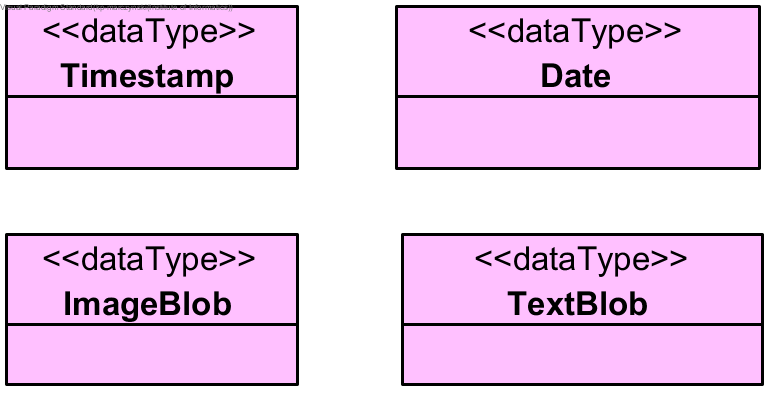
\includegraphics[scale=0.7]{../uml/class_diagrams/dataTypes.png}
        \caption{Typy danych - diagram klas (opr.wł).}\label{rysunek:class-diagram-data-types}
    \end{figure}
\end{minipage}

\begin{minipage}{\textwidth}
    \begin{figure}[H]
        \centering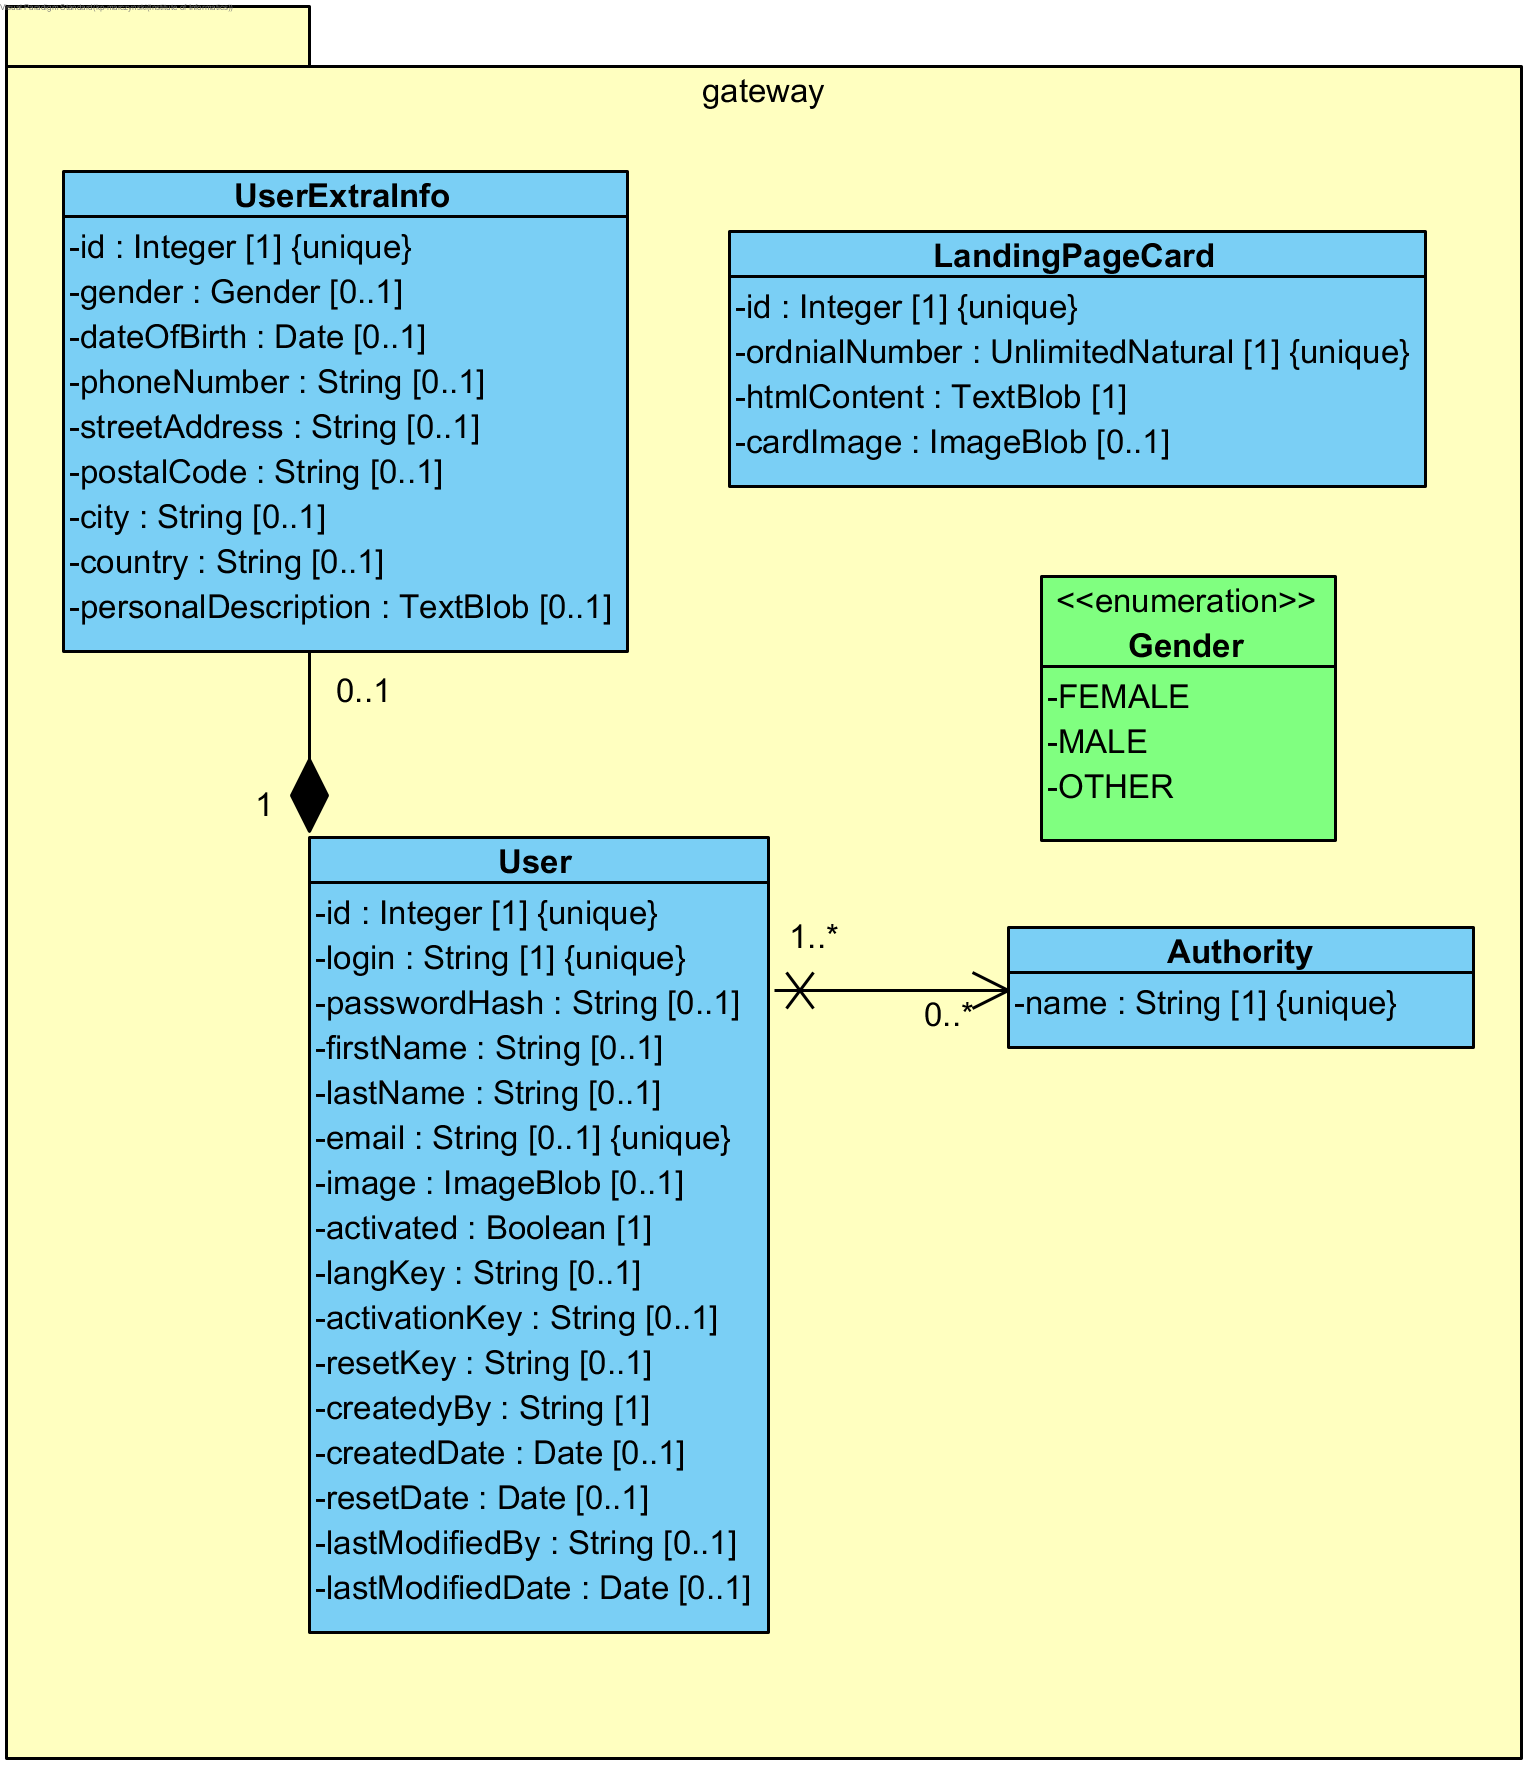
\includegraphics[scale=0.7]{../uml/class_diagrams/gateway.png}
        \caption{Gateway - diagram klas (opr.wł).}\label{rysunek:class-diagram-gateway}
    \end{figure}
\end{minipage}

\begin{minipage}{\textwidth}
    \begin{figure}[H]
        \centering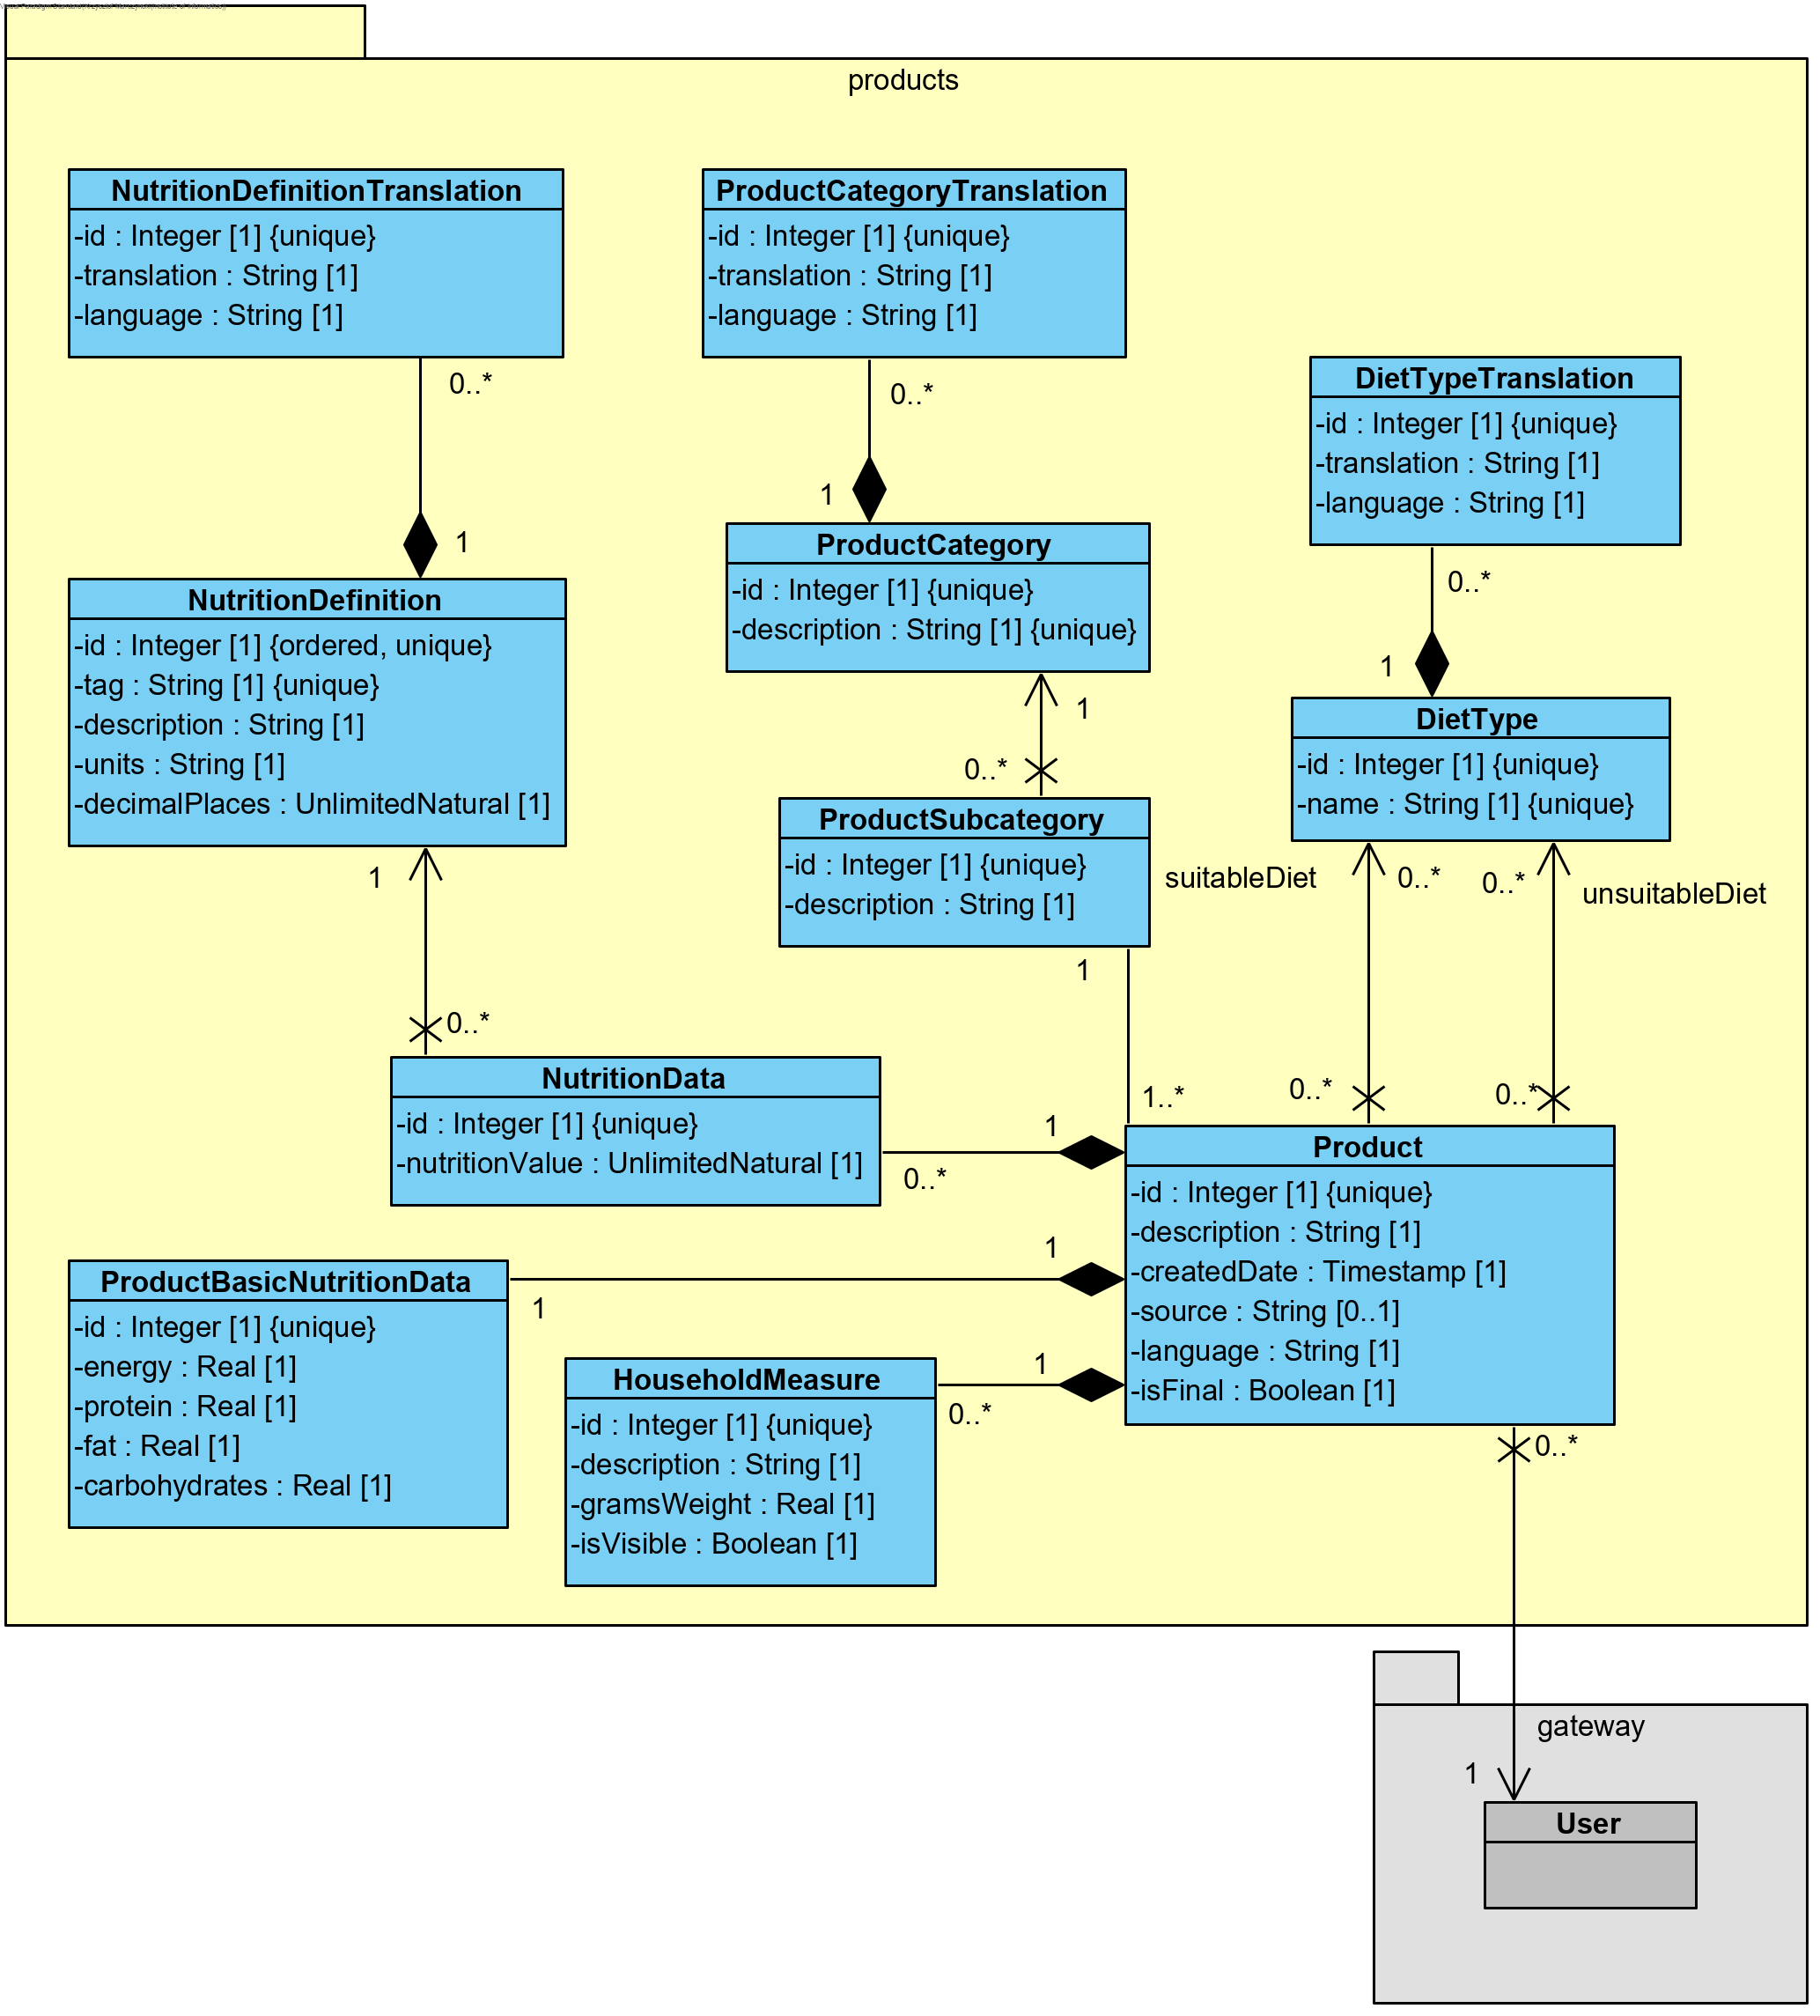
\includegraphics[scale=0.7]{../uml/class_diagrams/products.png}
        \caption{Produkty - diagram klas (opr.wł).}\label{rysunek:class-diagram-products}
    \end{figure}
\end{minipage}

\begin{minipage}{\textwidth}
    \begin{figure}[H]
        \centering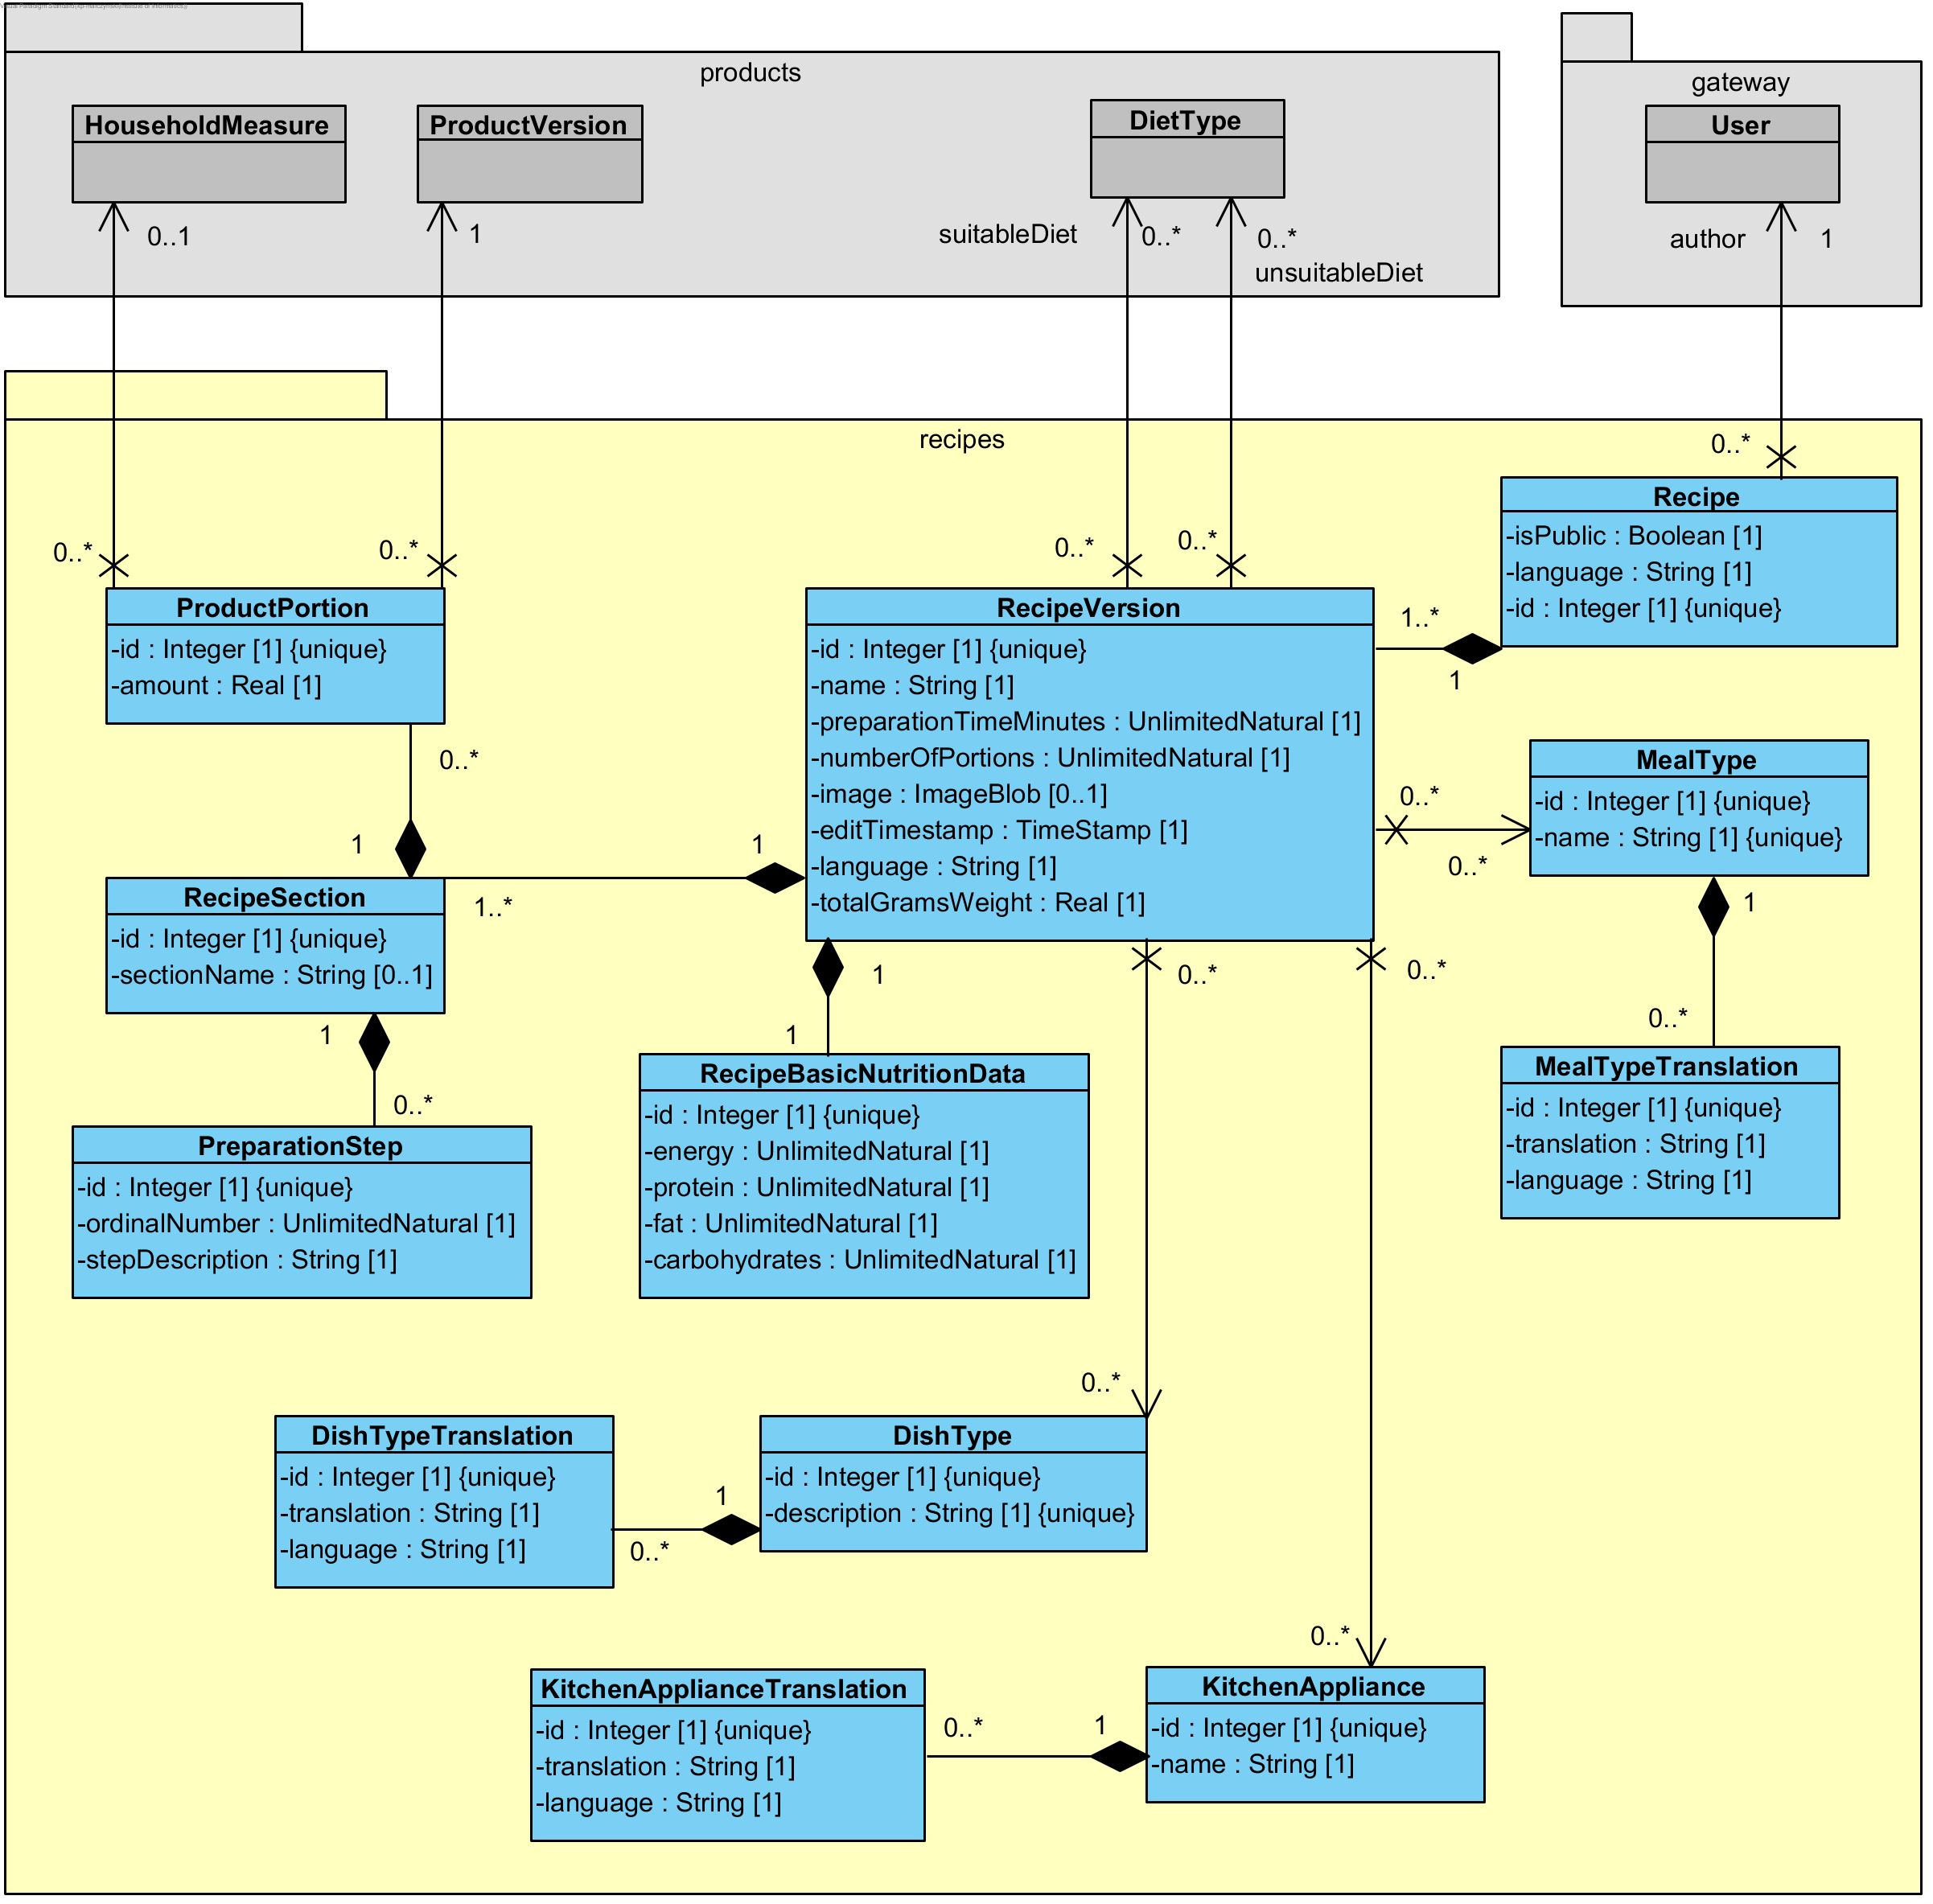
\includegraphics[scale=0.7]{../uml/class_diagrams/recipes.png}
        \caption{Przepisy - diagram klas (opr.wł).}\label{rysunek:class-diagram-recipes}
    \end{figure}
\end{minipage}

\begin{minipage}{\textwidth}
    \begin{figure}[H]
        \centering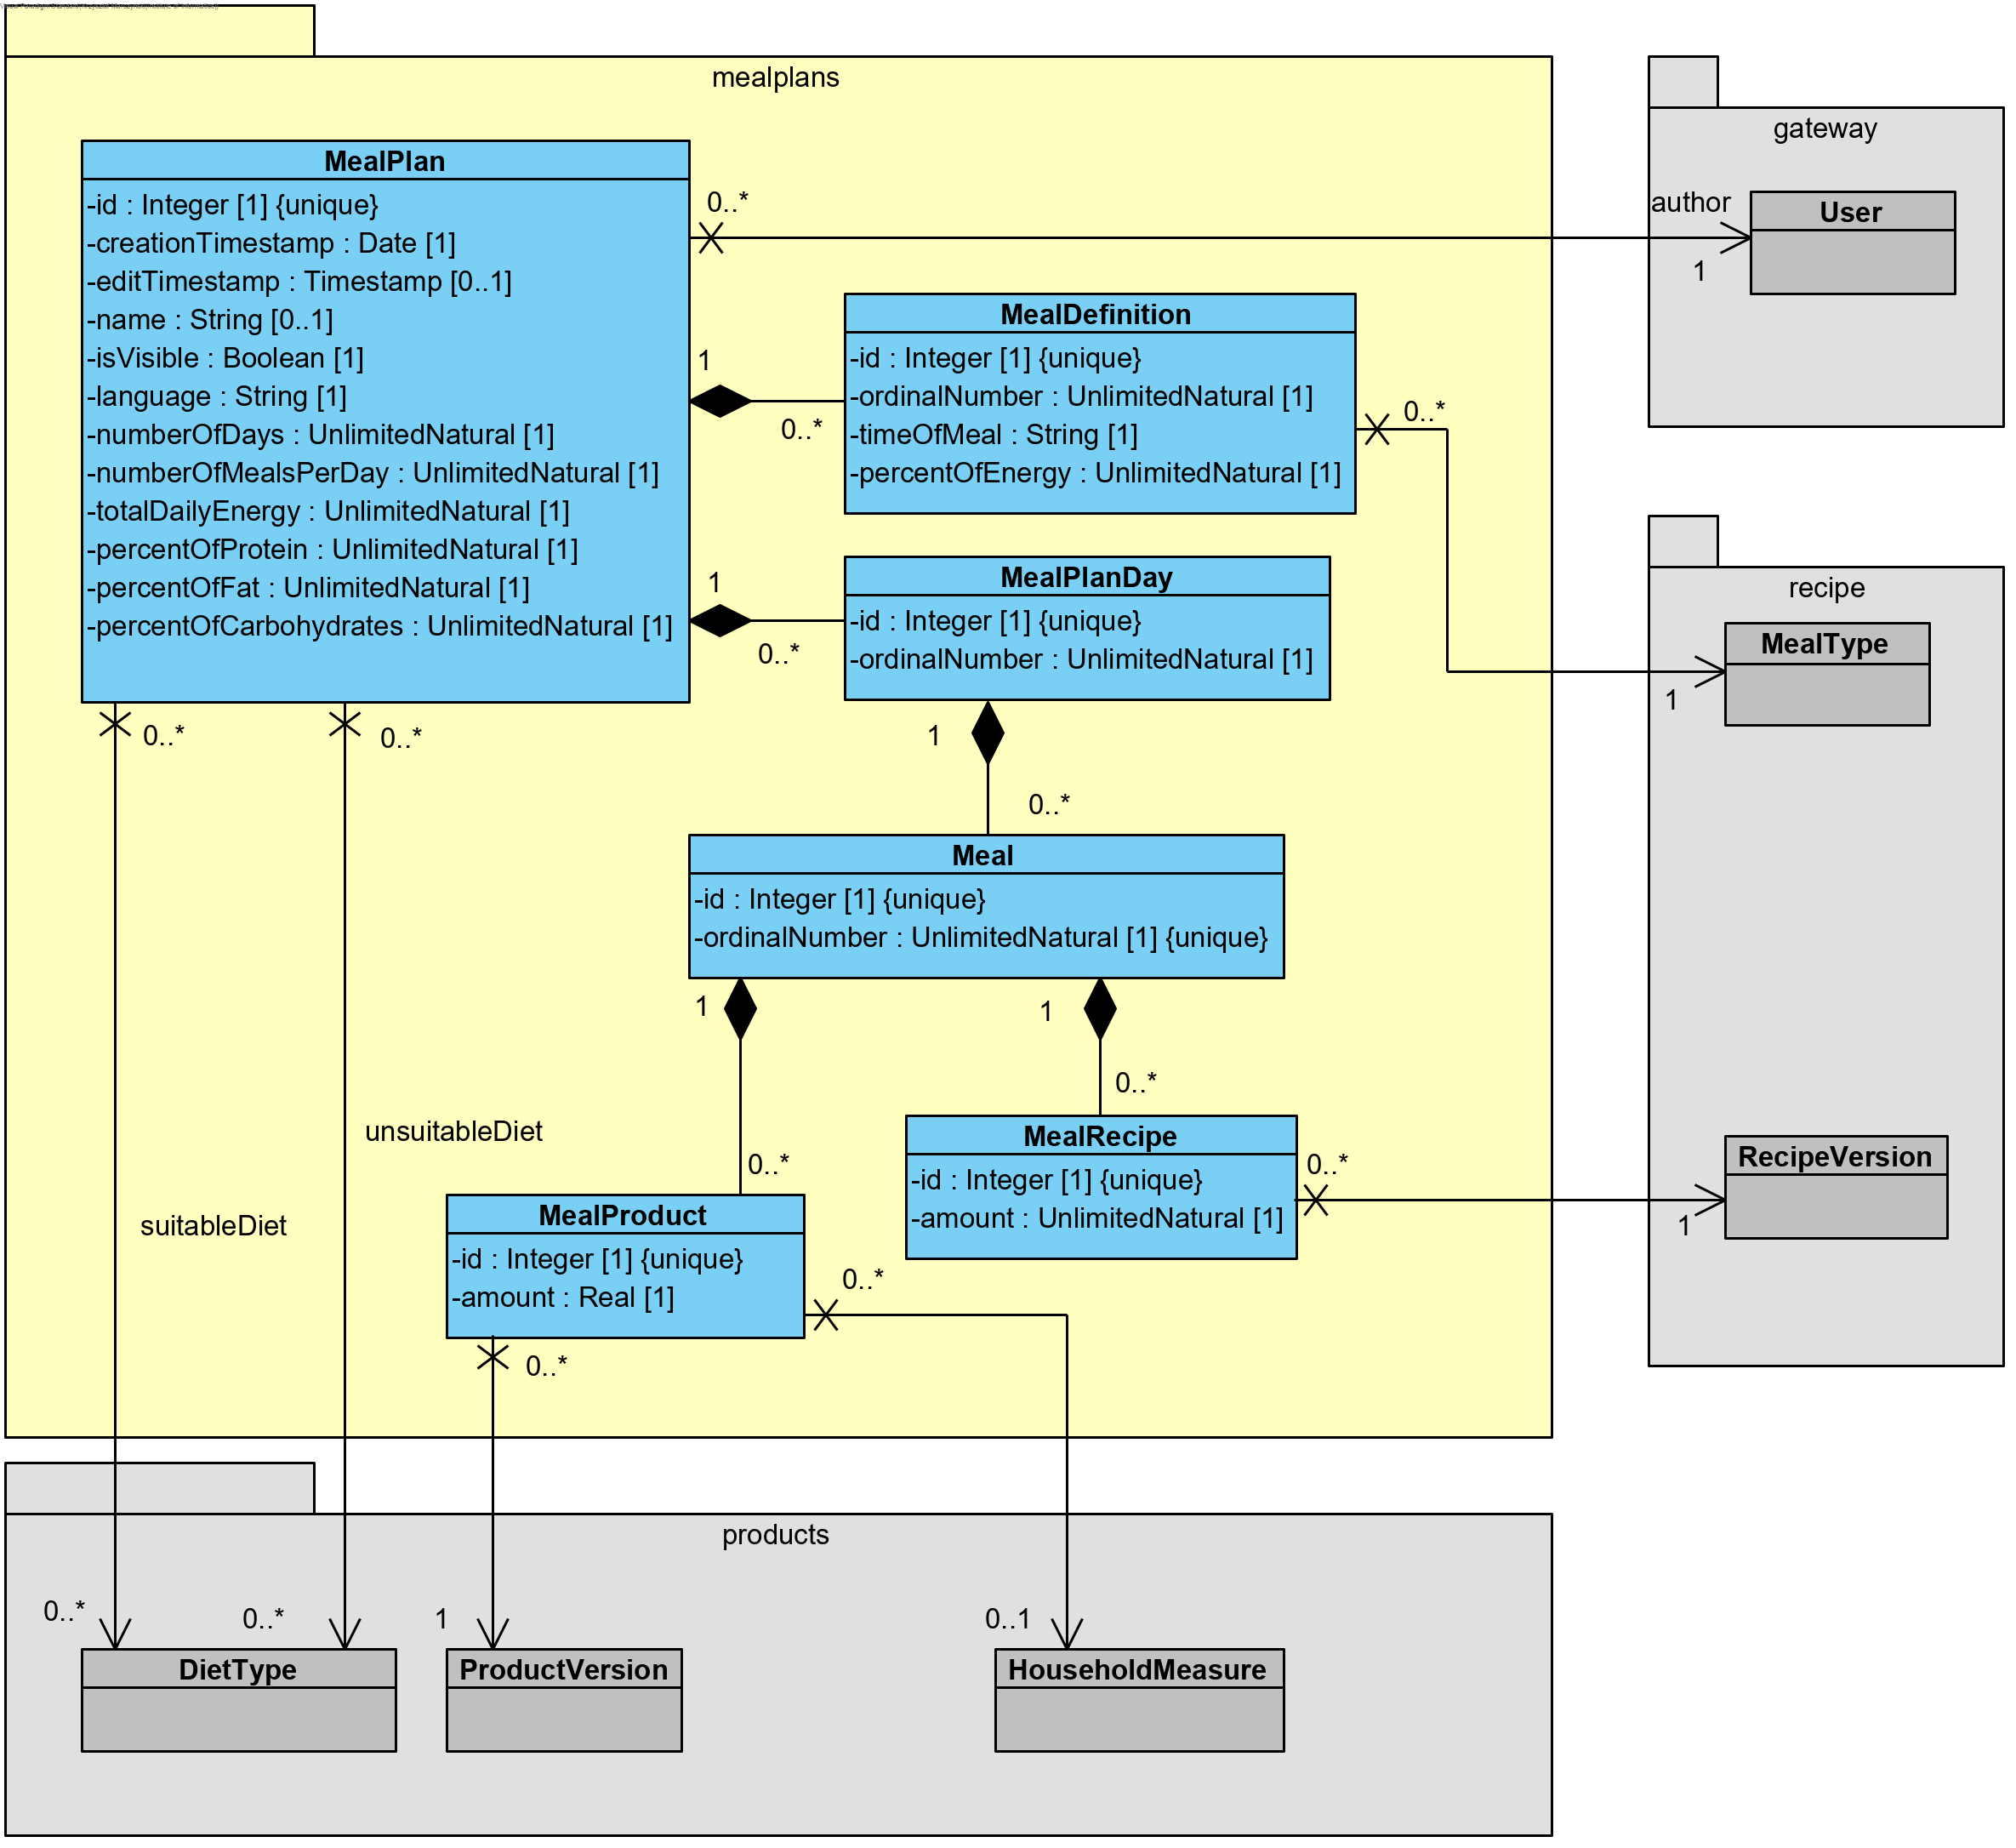
\includegraphics[scale=0.7]{../uml/class_diagrams/mealplans.png}
        \caption{Jadłospisy - diagram klas (opr.wł).}\label{rysunek:class-diagram-mealplans}
    \end{figure}
\end{minipage}

\begin{minipage}{\textwidth}
    \begin{figure}[H]
        \centering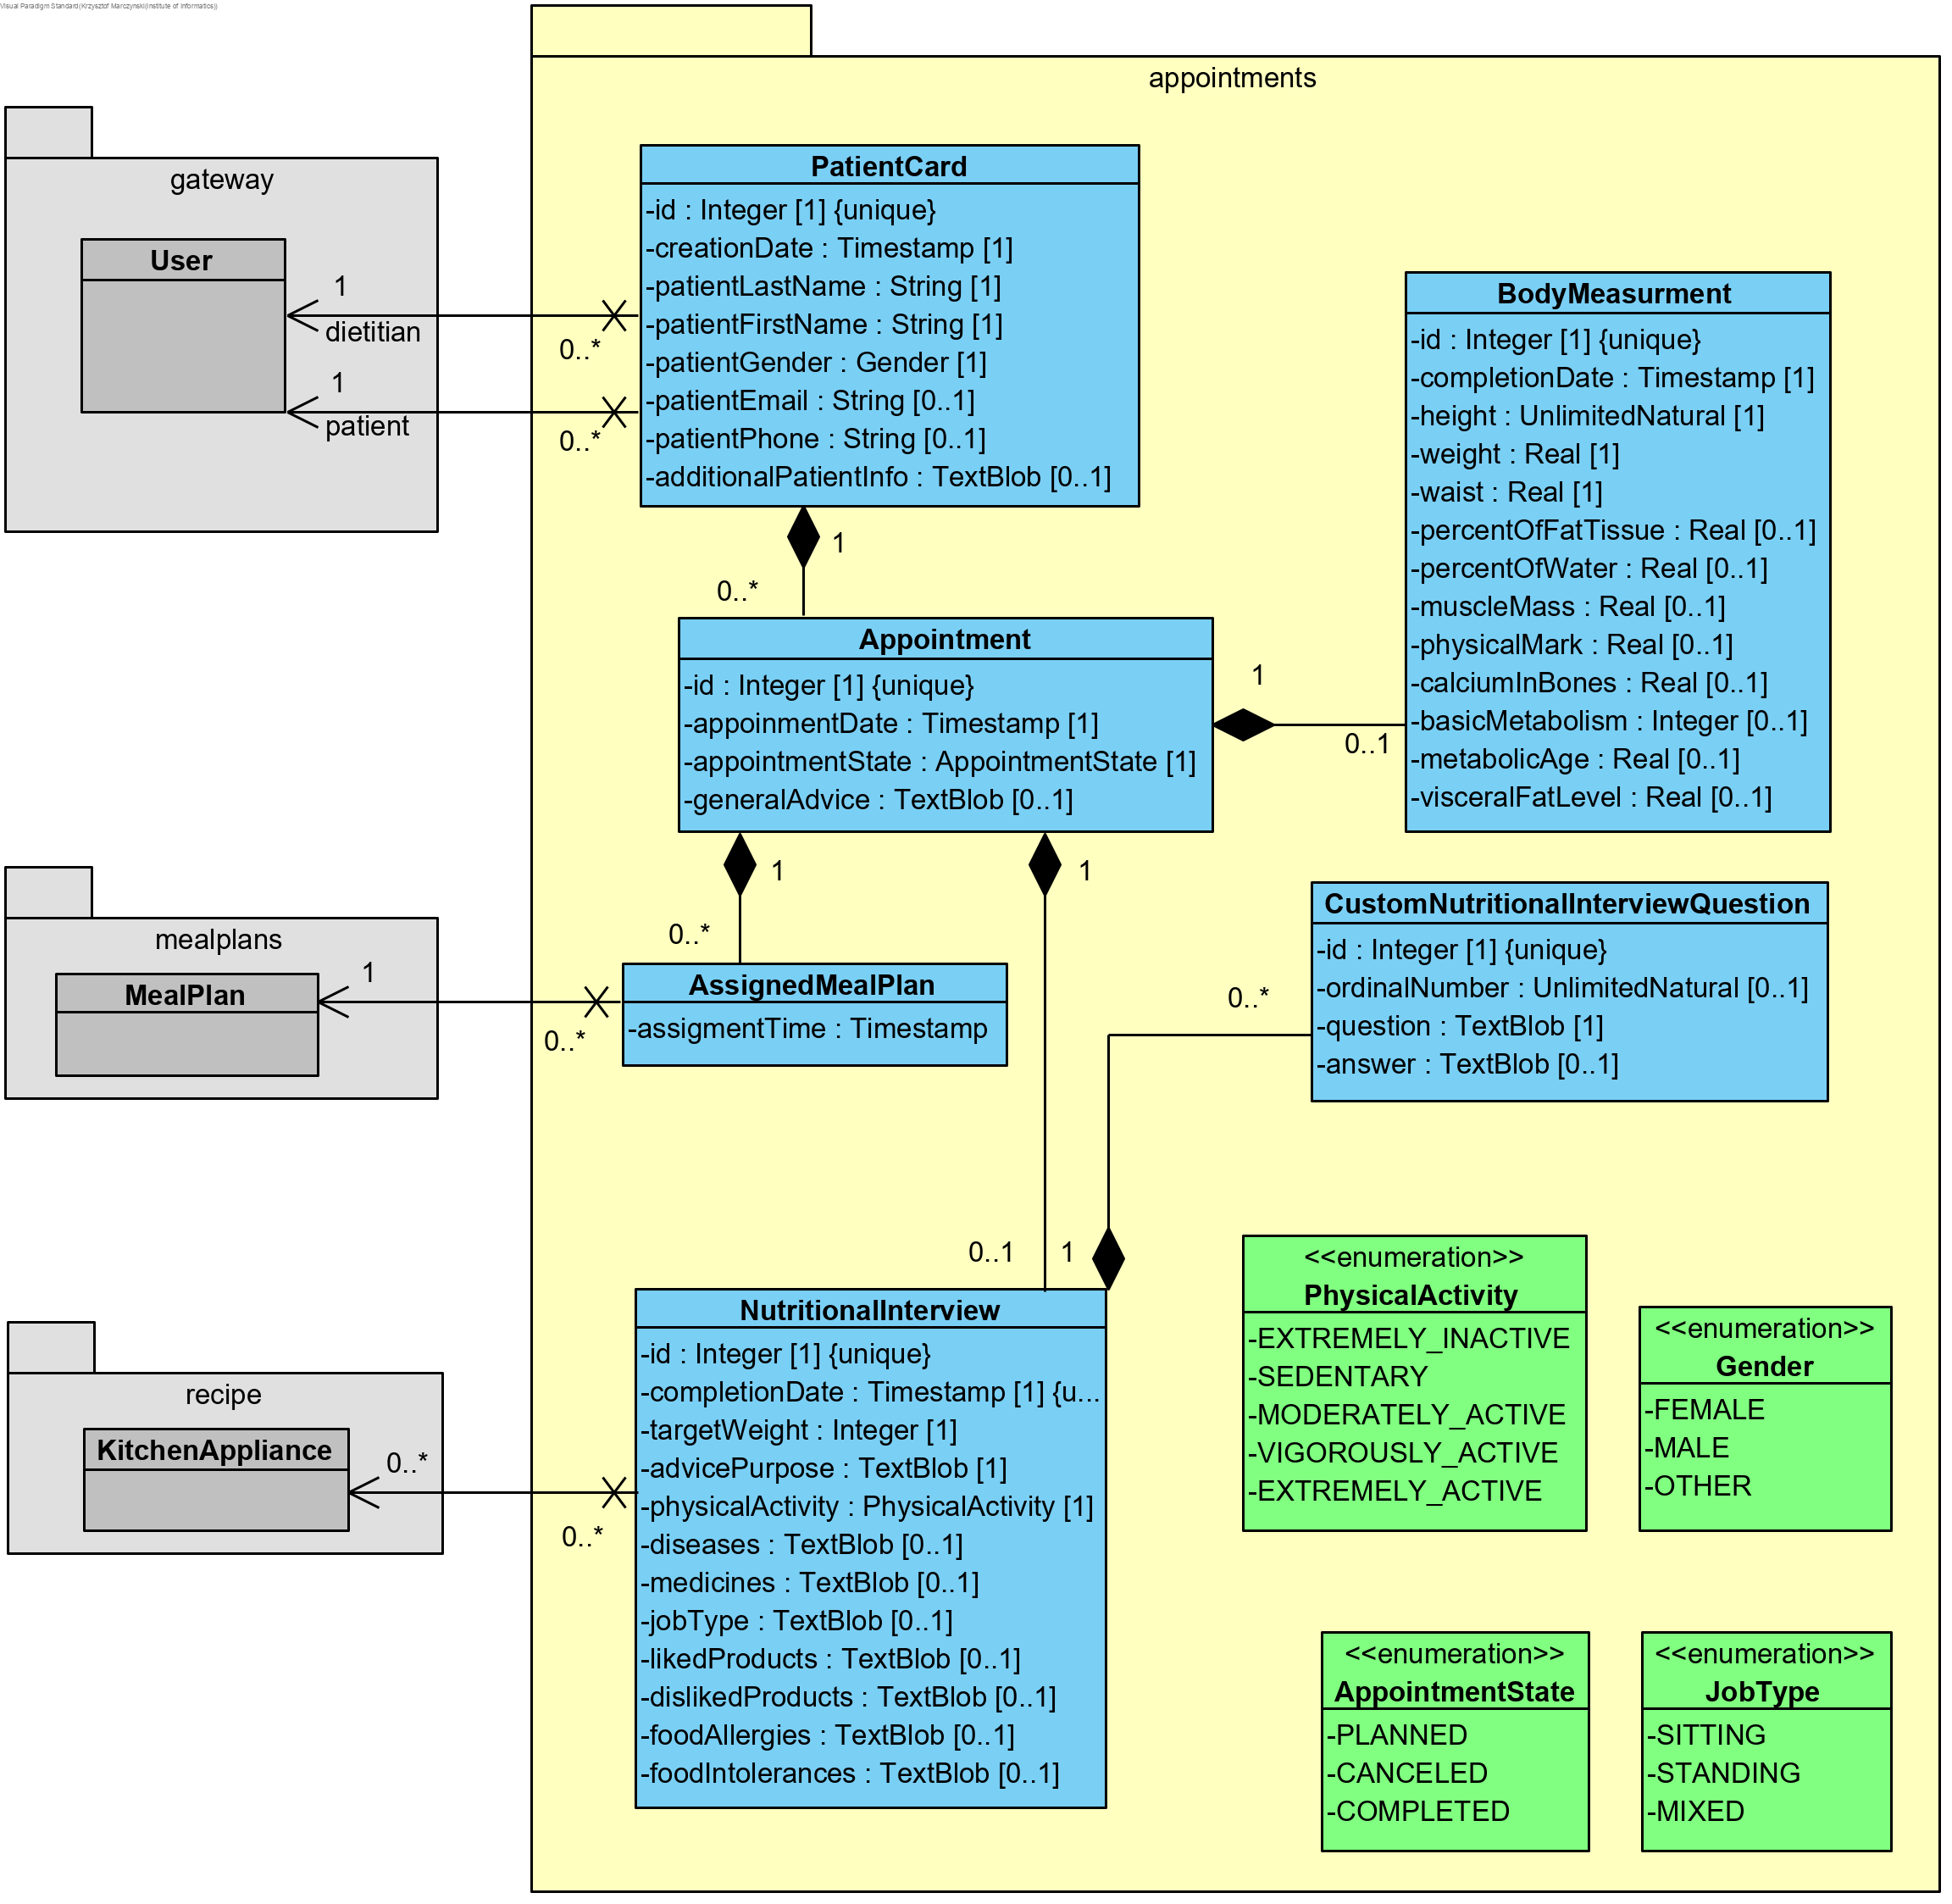
\includegraphics[scale=0.7]{../uml/class_diagrams/appointments.png}
        \caption{Wizyty - diagram klas (opr.wł).}\label{rysunek:class-diagram-appointments}
    \end{figure}
\end{minipage}

\section{Opis podstawowej architektury systemu}\label{sec:basicArchitecture}
\todo{Opisać, że to aplikacja webowa w architekturze mikroserwisów
Wyszczególnienie modułów;
Diagram rozmieszczenia, wzorce projektowe}

%https://martinfowler.com/eaaDev/TemporalObject.html
\thispagestyle{normal}

    \chapter{Projekt}
\section{Przypadki użycia}
\section{Model interfejsu}
\begin{minipage}{\textwidth}
    \begin{figure}[H]
        \centering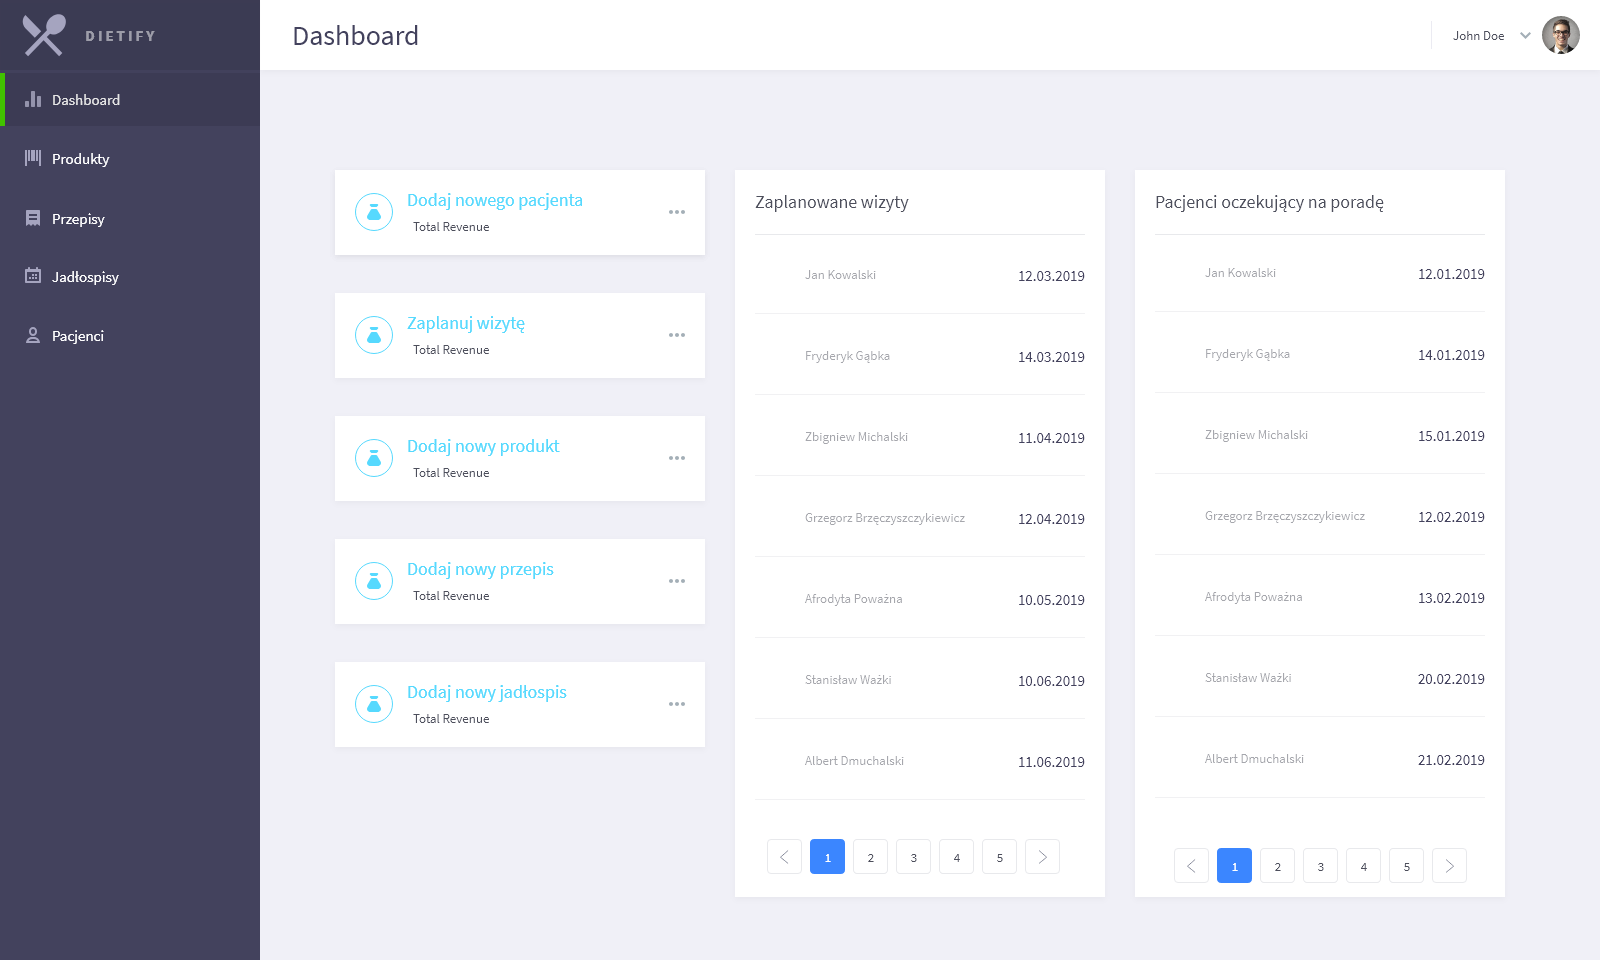
\includegraphics[width=0.9\textwidth]{img/mockups/mockup1.png}
        \caption{Mockup1 (opr.w).}\label{rysunek:mockup1}
    \end{figure}
\end{minipage}

\begin{minipage}{\textwidth}
    \begin{figure}[H]
        \centering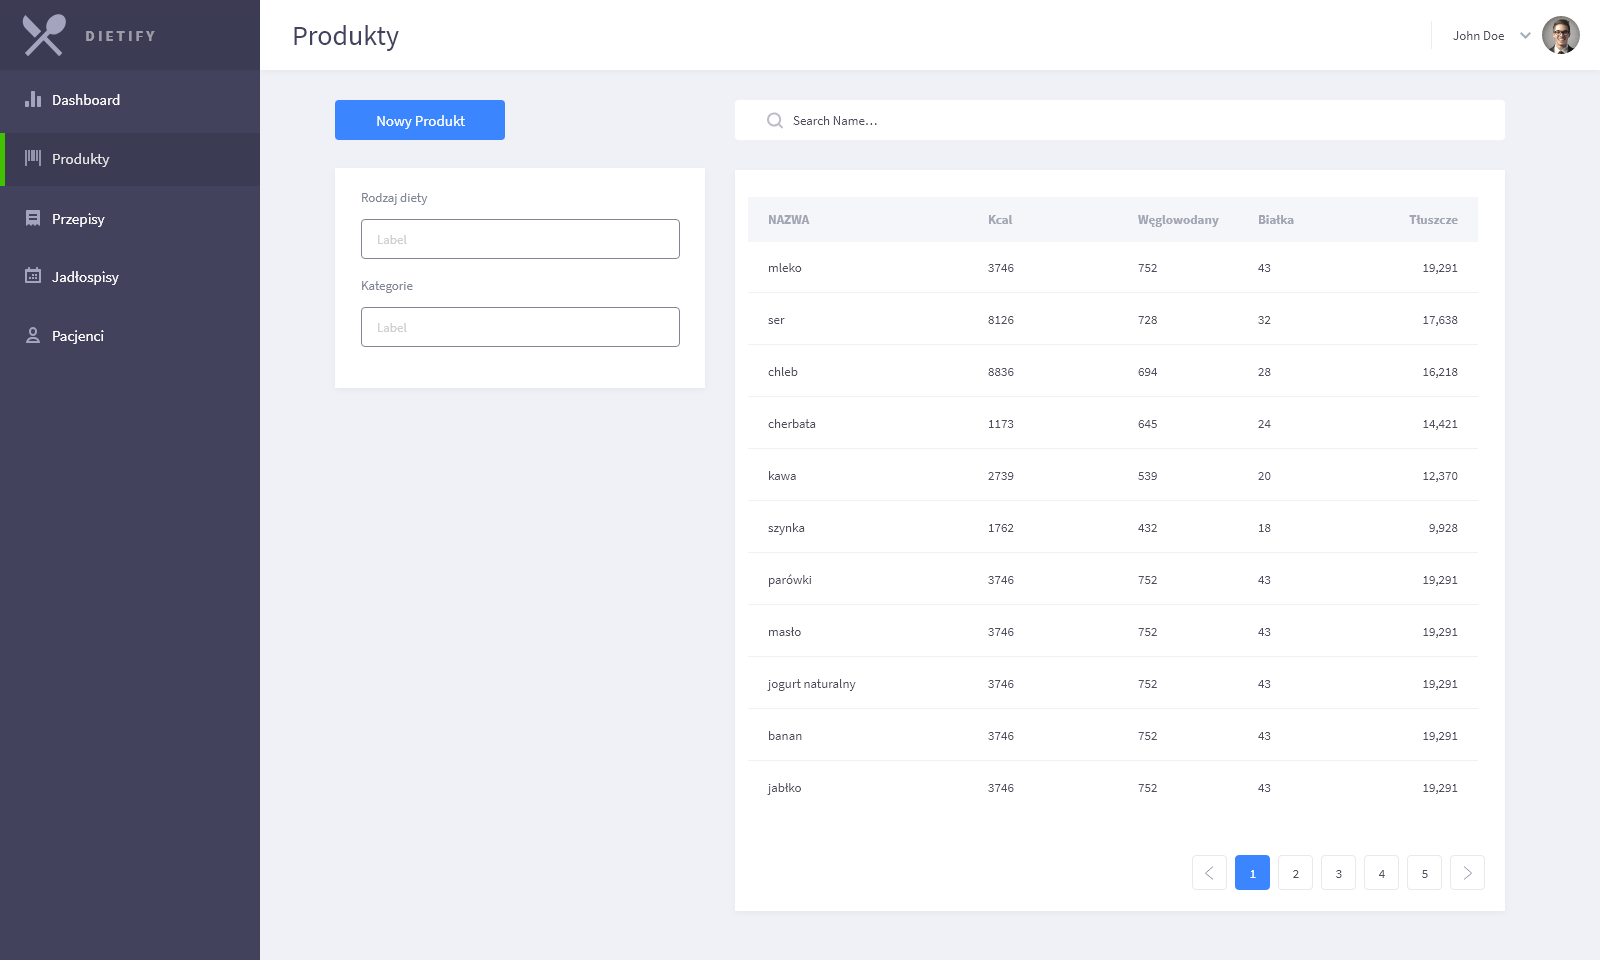
\includegraphics[width=0.9\textwidth]{img/mockups/mockup2.png}
        \caption{Mockup2 (opr.w).}\label{rysunek:mockup2}
    \end{figure}
\end{minipage}

\begin{minipage}{\textwidth}
    \begin{figure}[H]
        \centering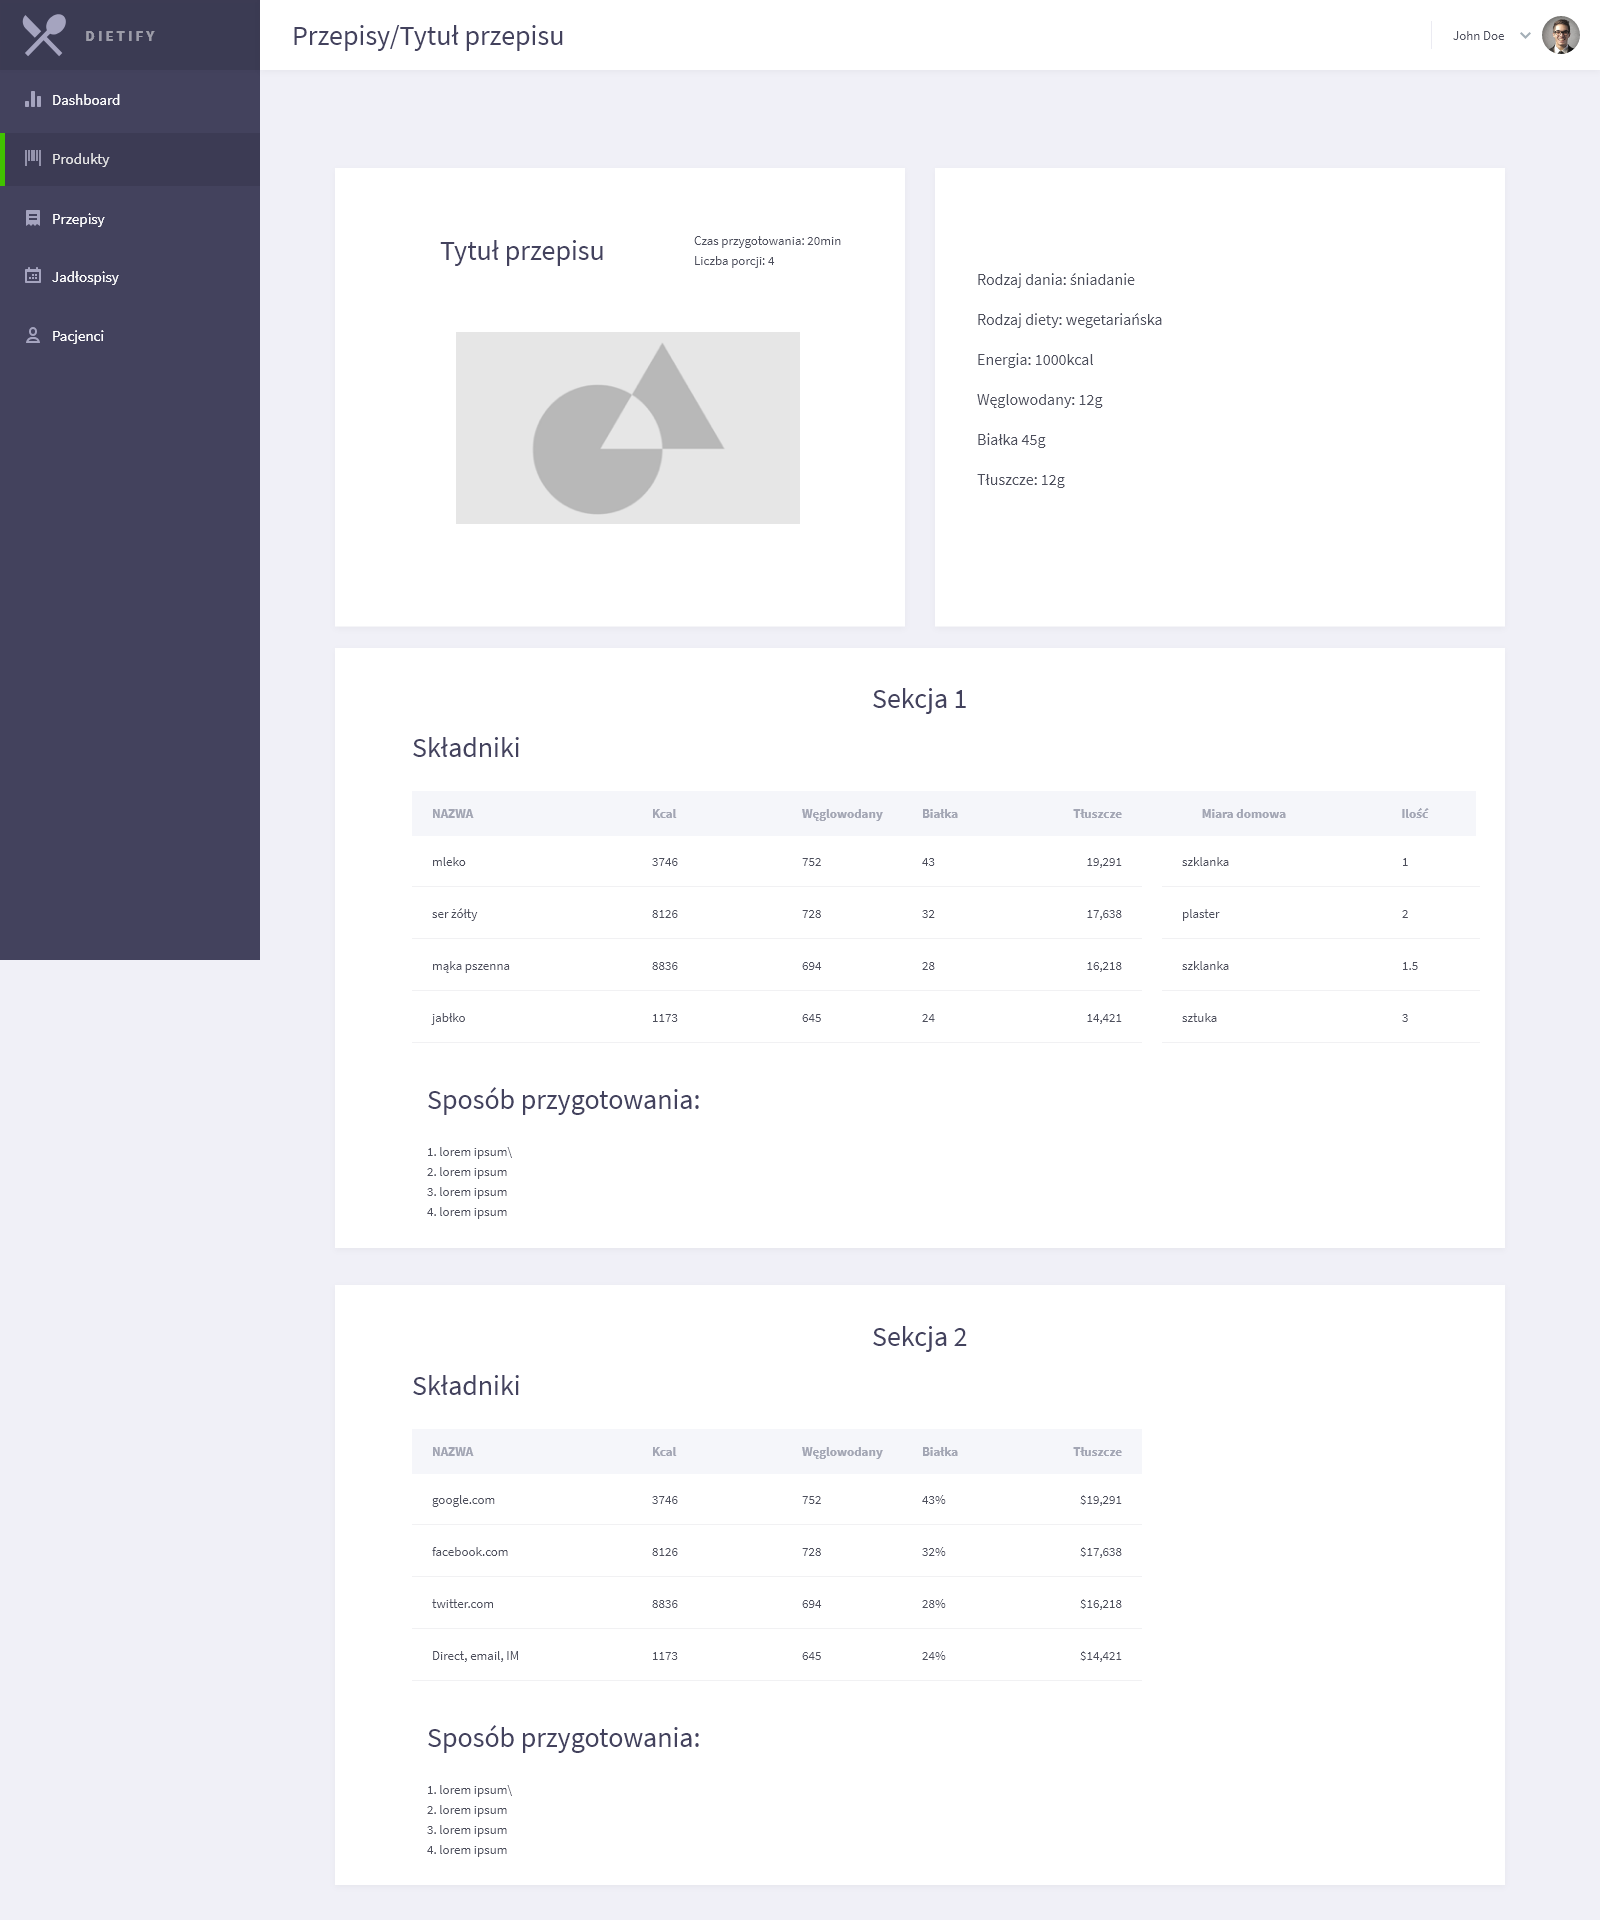
\includegraphics[width=0.9\textwidth]{img/mockups/mockup3.png}
        \caption{Mockup3 (opr.w).}\label{rysunek:mockup3}
    \end{figure}
\end{minipage}

\begin{minipage}{\textwidth}
    \begin{figure}[H]
        \centering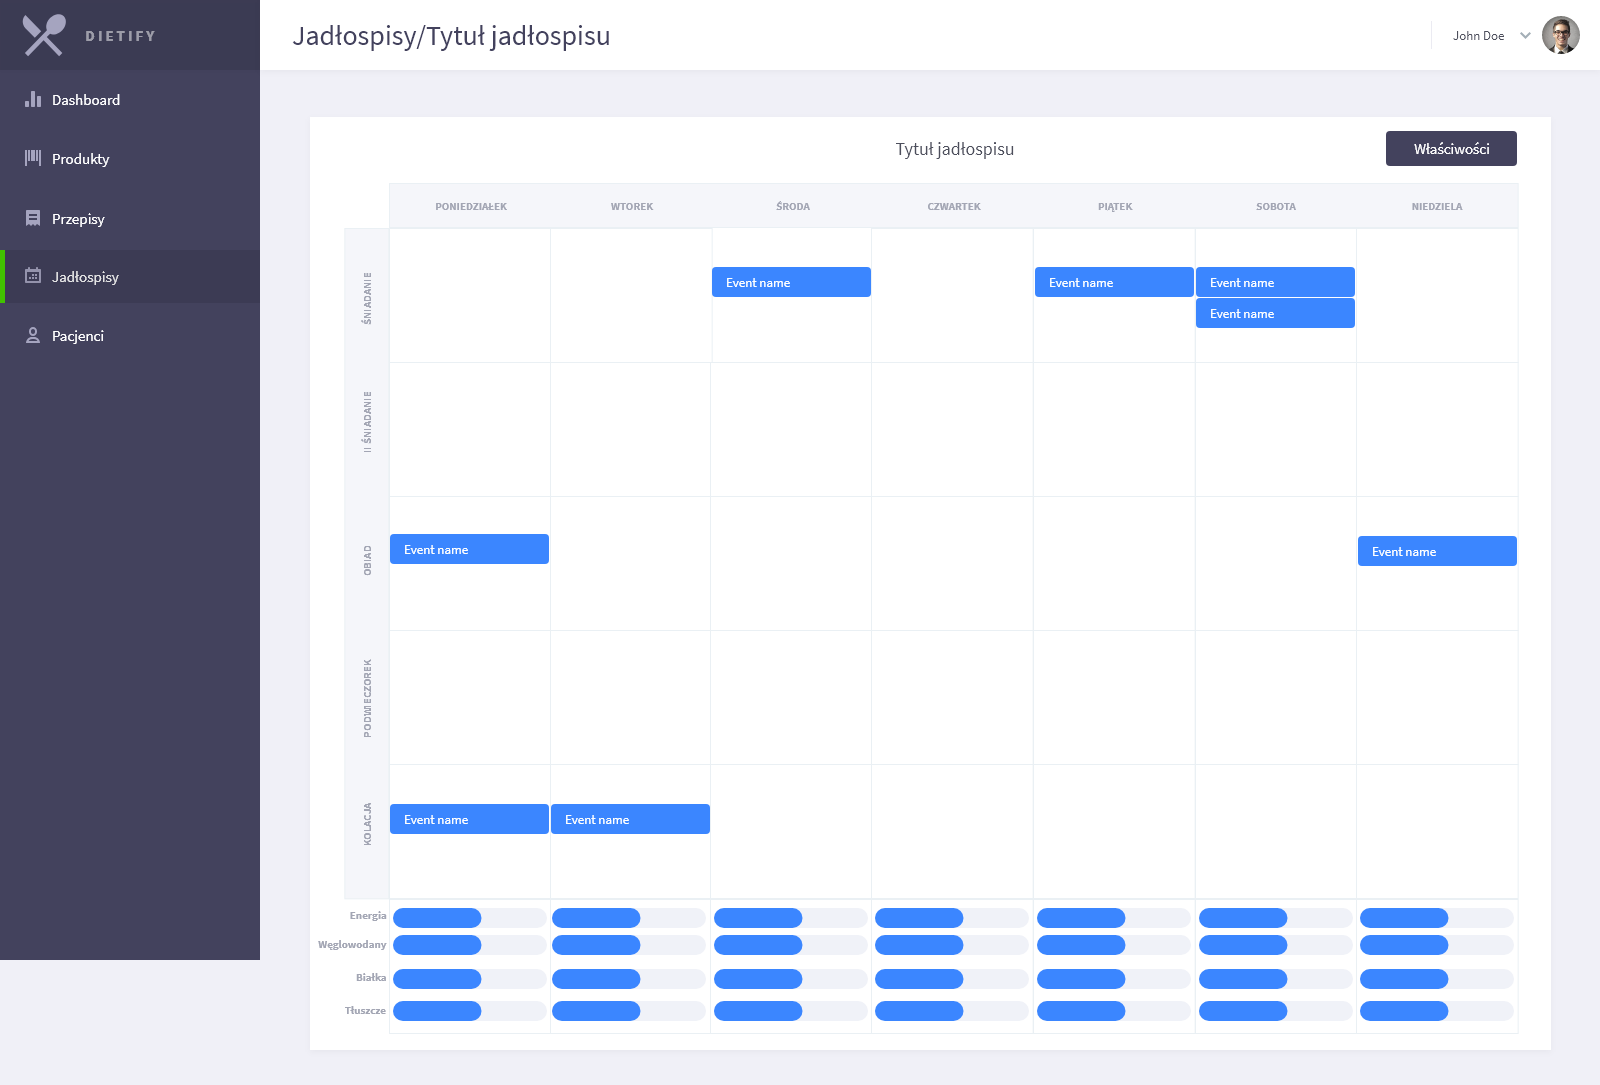
\includegraphics[width=0.9\textwidth]{img/mockups/mockup4.png}
        \caption{Mockup4 (opr.w).}\label{rysunek:mockup4}
    \end{figure}
\end{minipage}

\begin{minipage}{\textwidth}
    \begin{figure}[H]
        \centering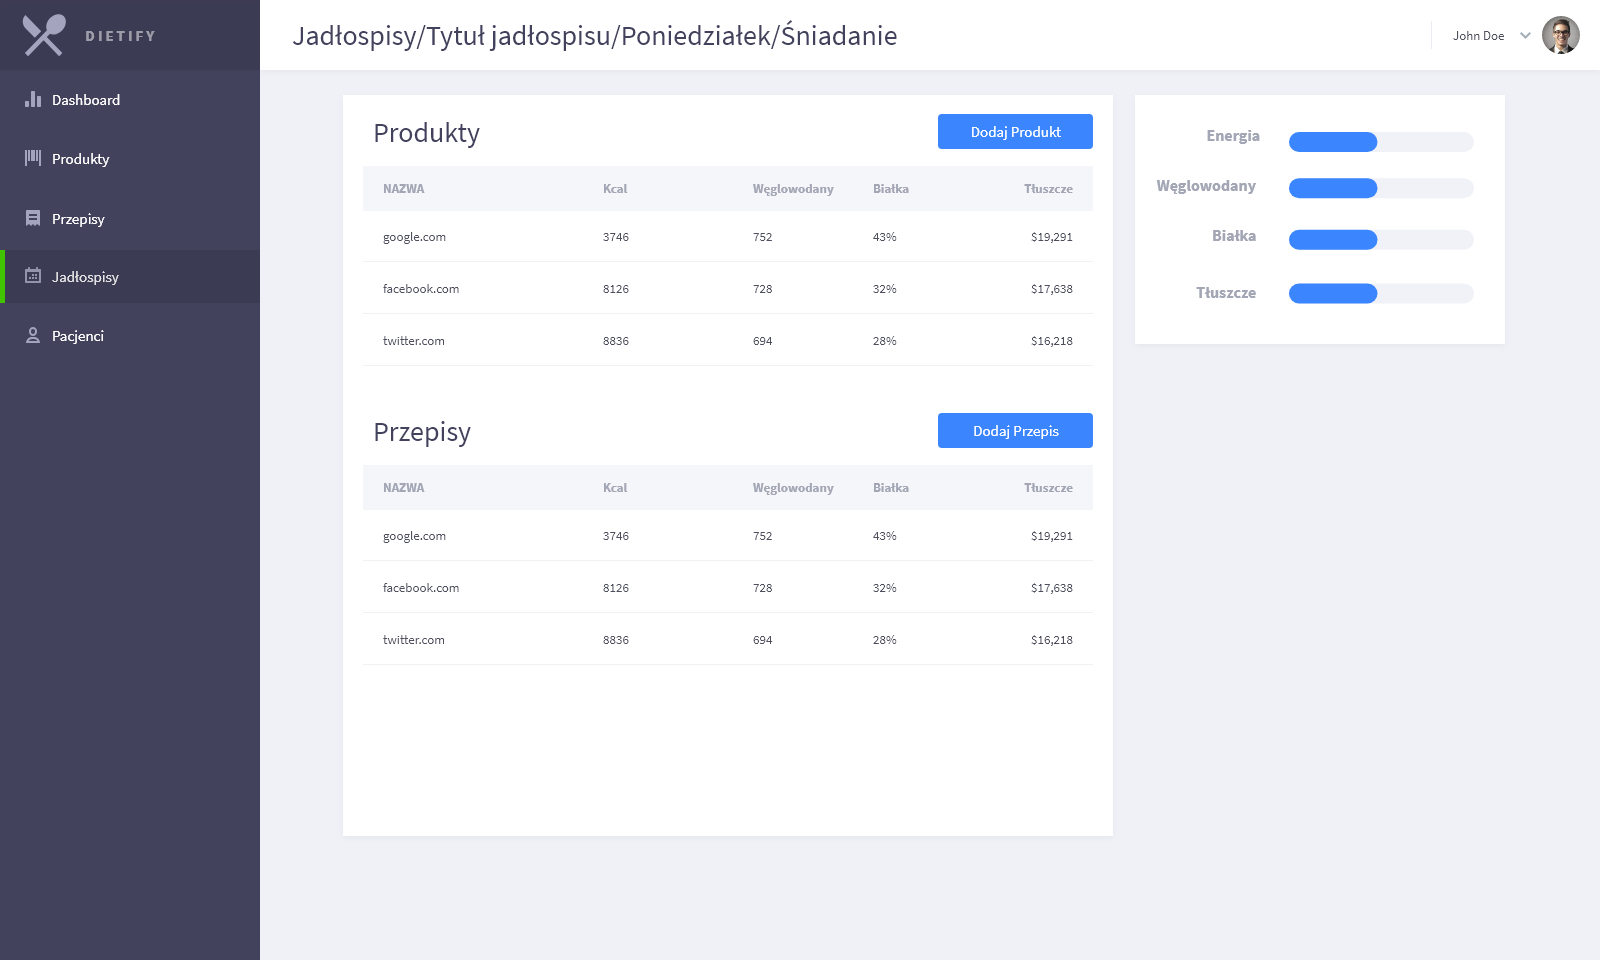
\includegraphics[width=0.9\textwidth]{img/mockups/mockup5.png}
        \caption{Mockup5 (opr.w).}\label{rysunek:mockup5}
    \end{figure}
\end{minipage}

\begin{minipage}{\textwidth}
    \begin{figure}[H]
        \centering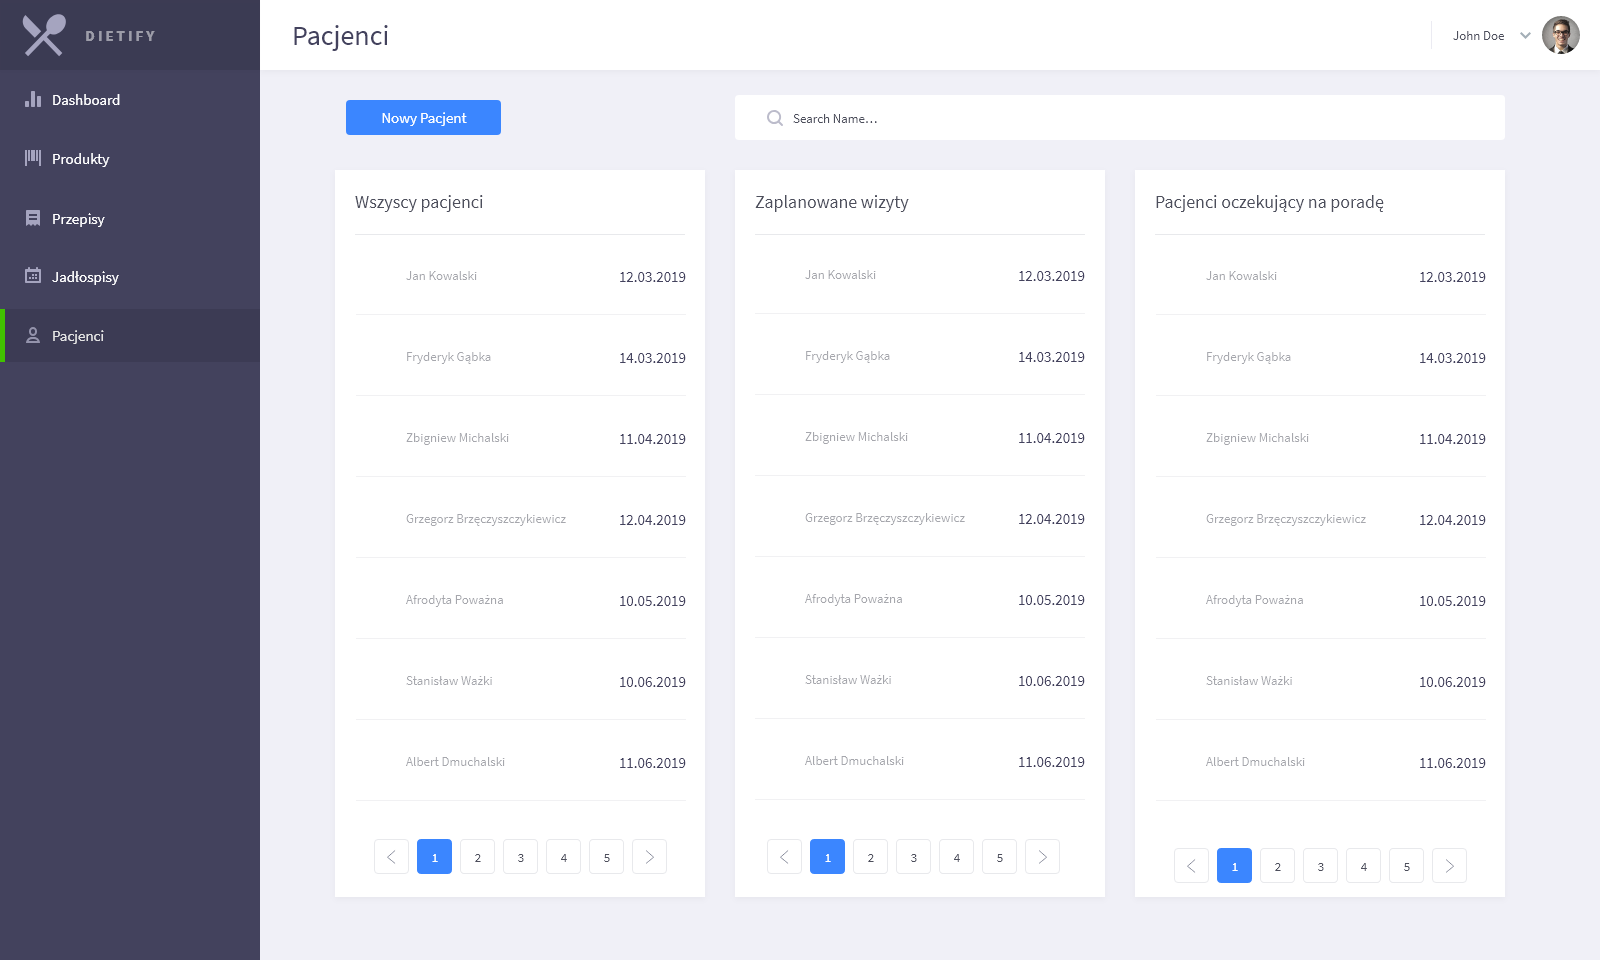
\includegraphics[width=0.9\textwidth]{img/mockups/mockup6.png}
        \caption{Mockup6 (opr.w).}\label{rysunek:mockup6}
    \end{figure}
\end{minipage}

\begin{minipage}{\textwidth}
    \begin{figure}[H]
        \centering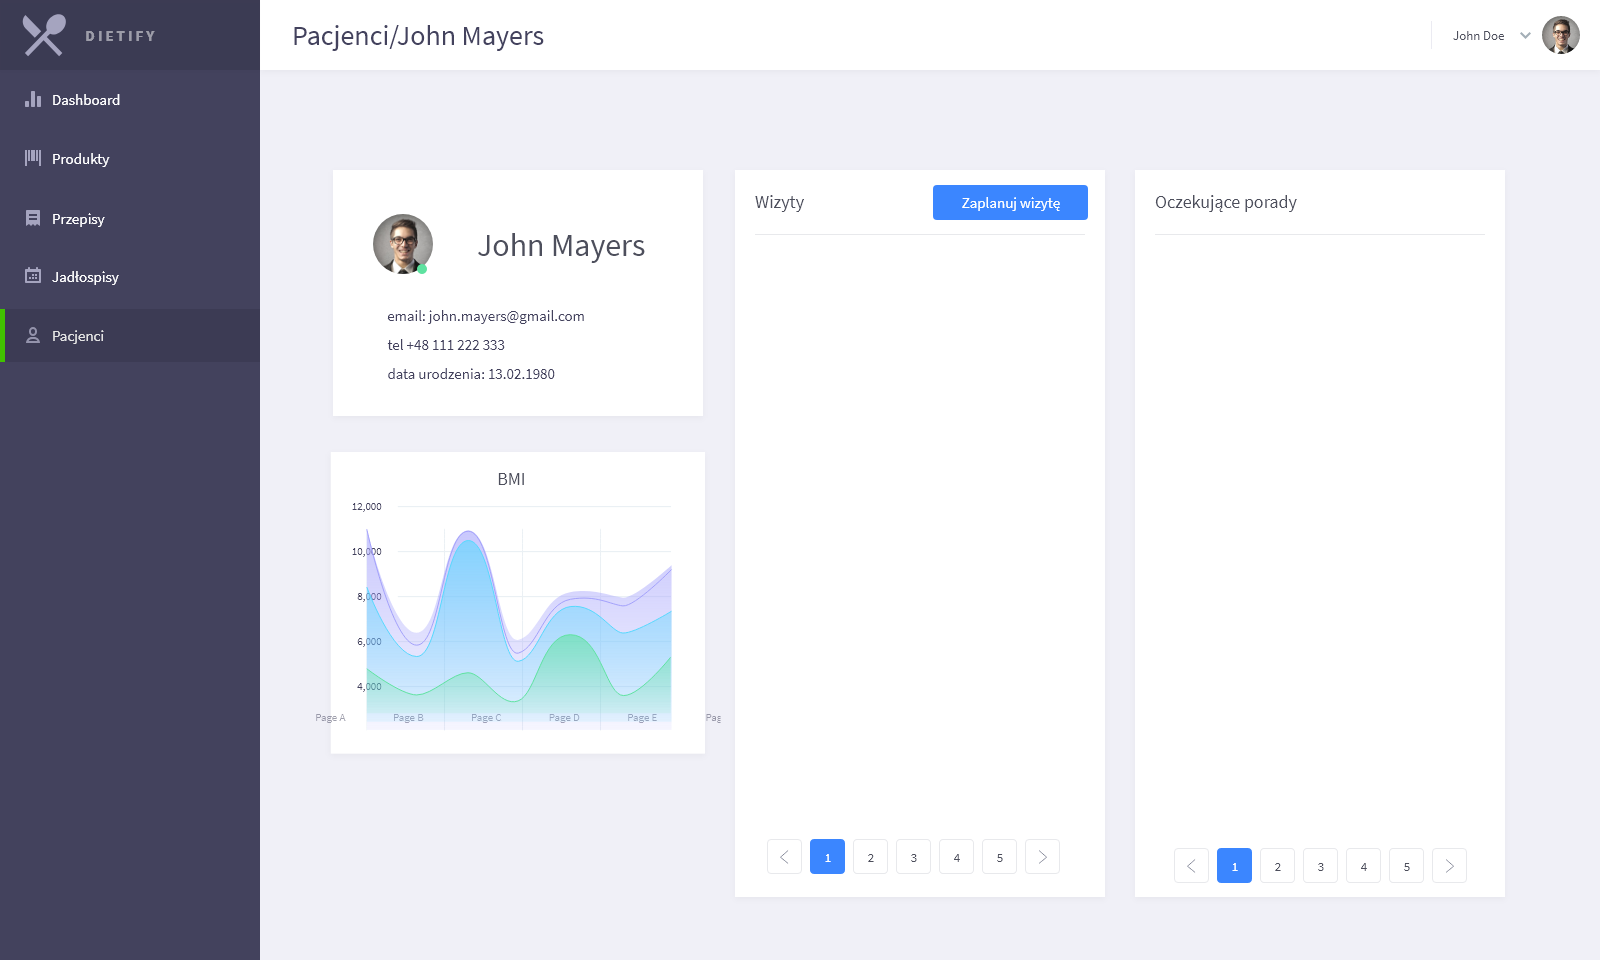
\includegraphics[width=0.9\textwidth]{img/mockups/mockup7.png}
        \caption{Mockup7 (opr.w).}\label{rysunek:mockup7}
    \end{figure}
\end{minipage}

\begin{minipage}{\textwidth}
    \begin{figure}[H]
        \centering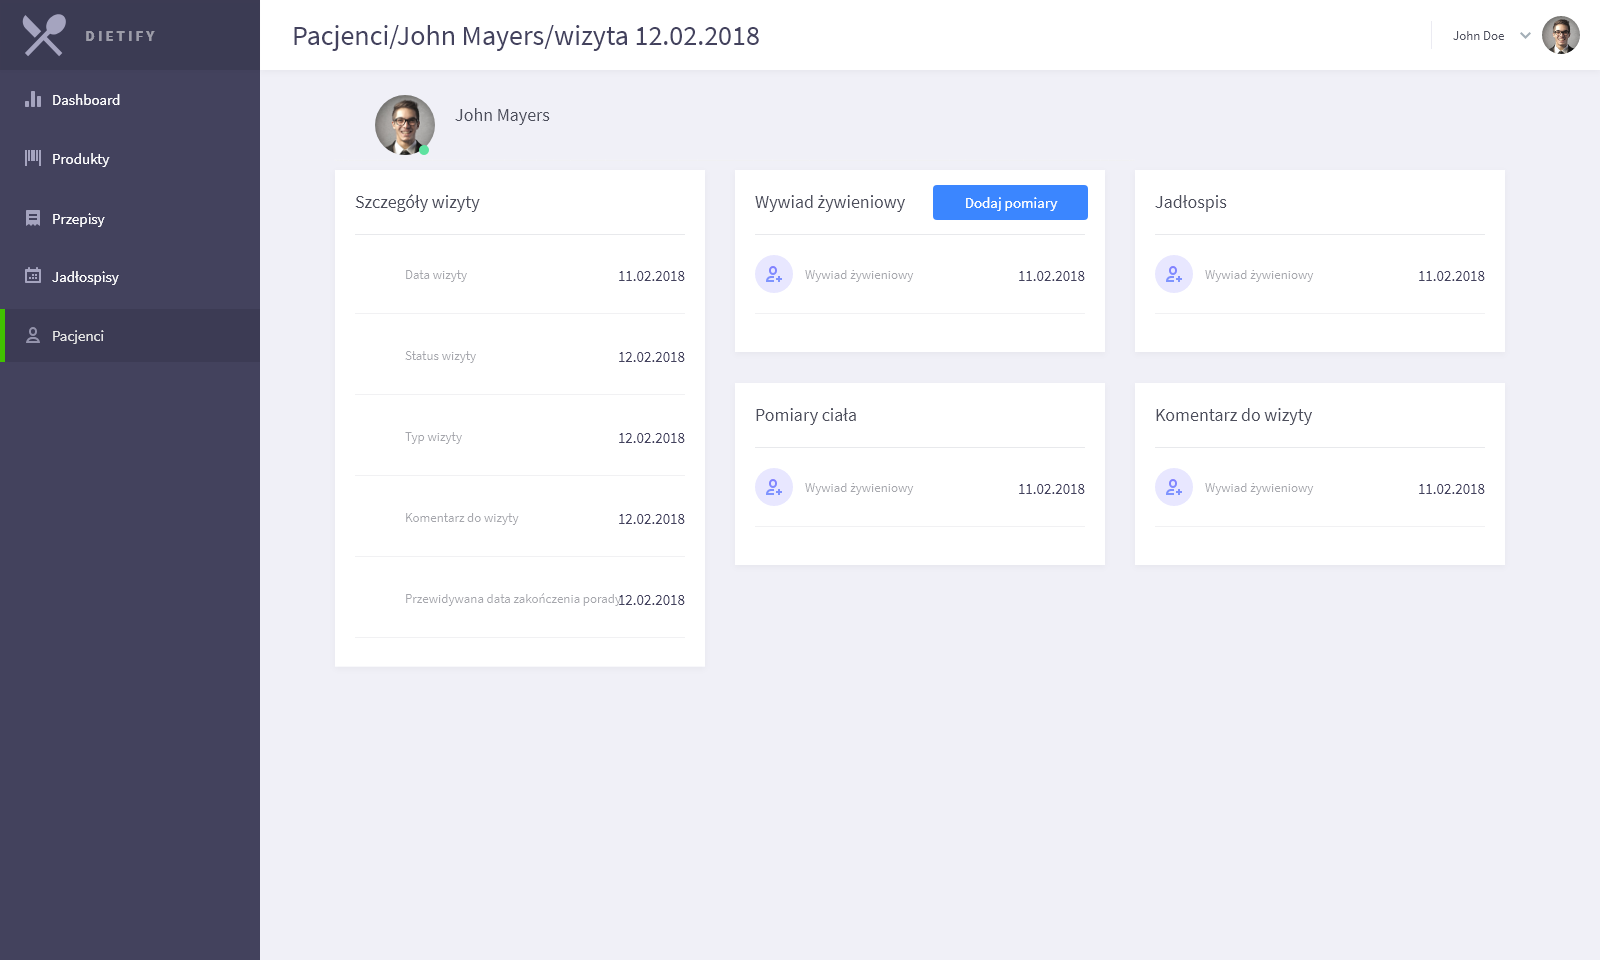
\includegraphics[width=0.9\textwidth]{img/mockups/mockup8.png}
        \caption{Mockup8 (opr.w).}\label{rysunek:mockup8}
    \end{figure}
\end{minipage}

\begin{minipage}{\textwidth}
    \begin{figure}[H]
        \centering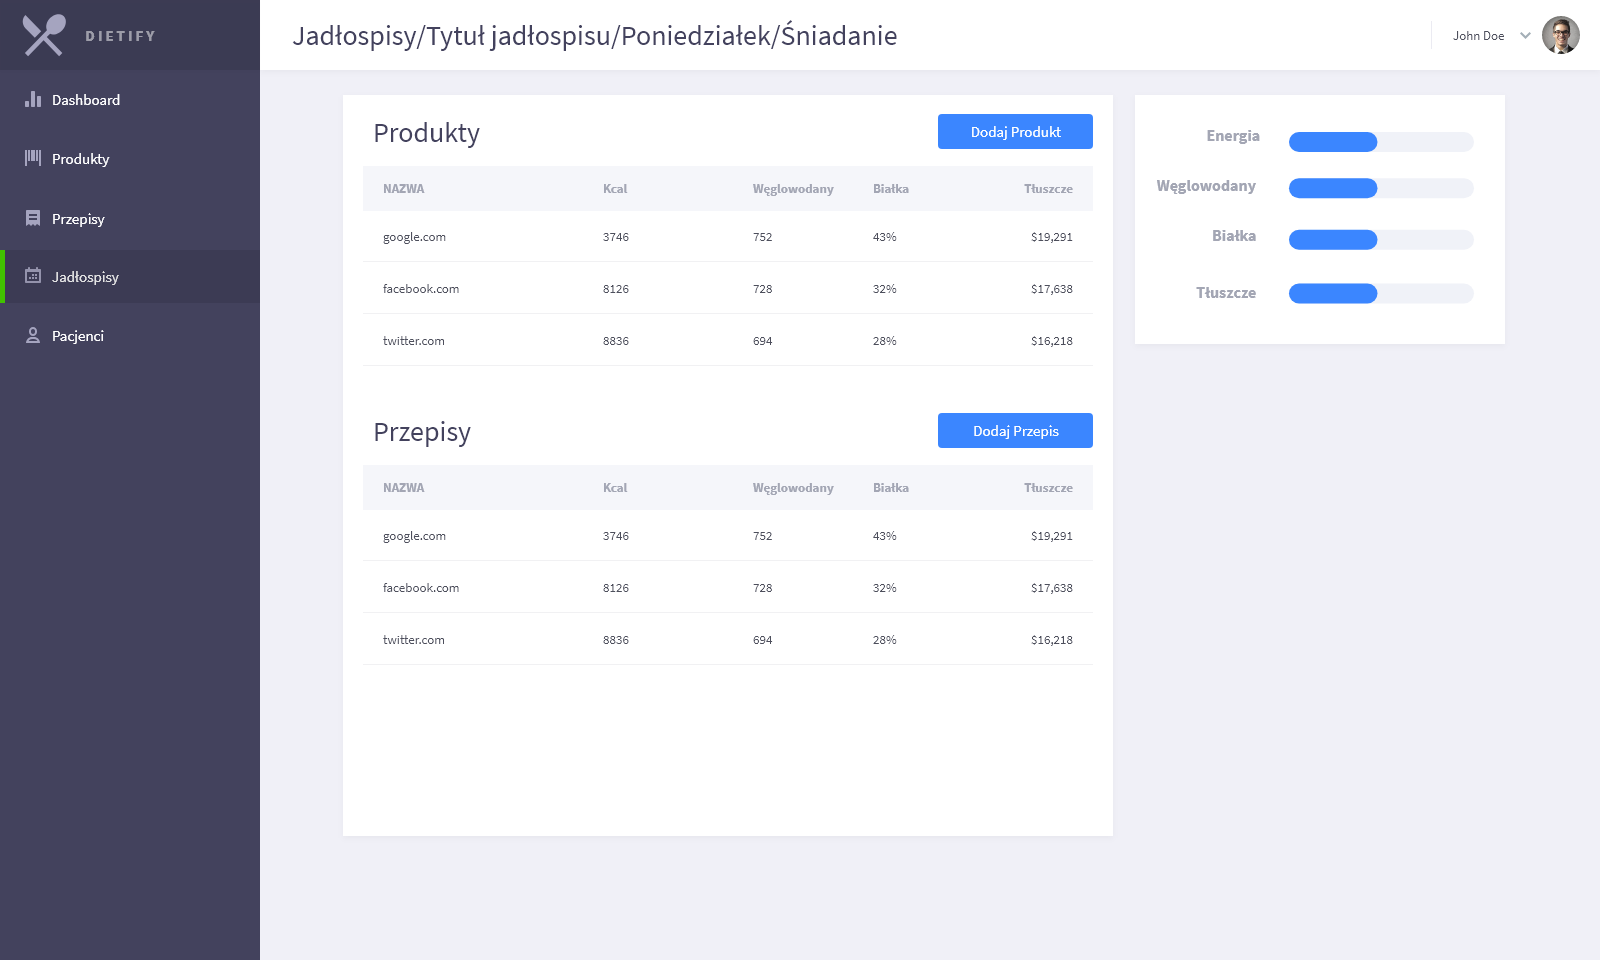
\includegraphics[width=0.9\textwidth]{img/mockups/mockup9.png}
        \caption{Mockup9 (opr.w).}\label{rysunek:mockup9}
    \end{figure}
\end{minipage}

\begin{minipage}{\textwidth}
    \begin{figure}[H]
        \centering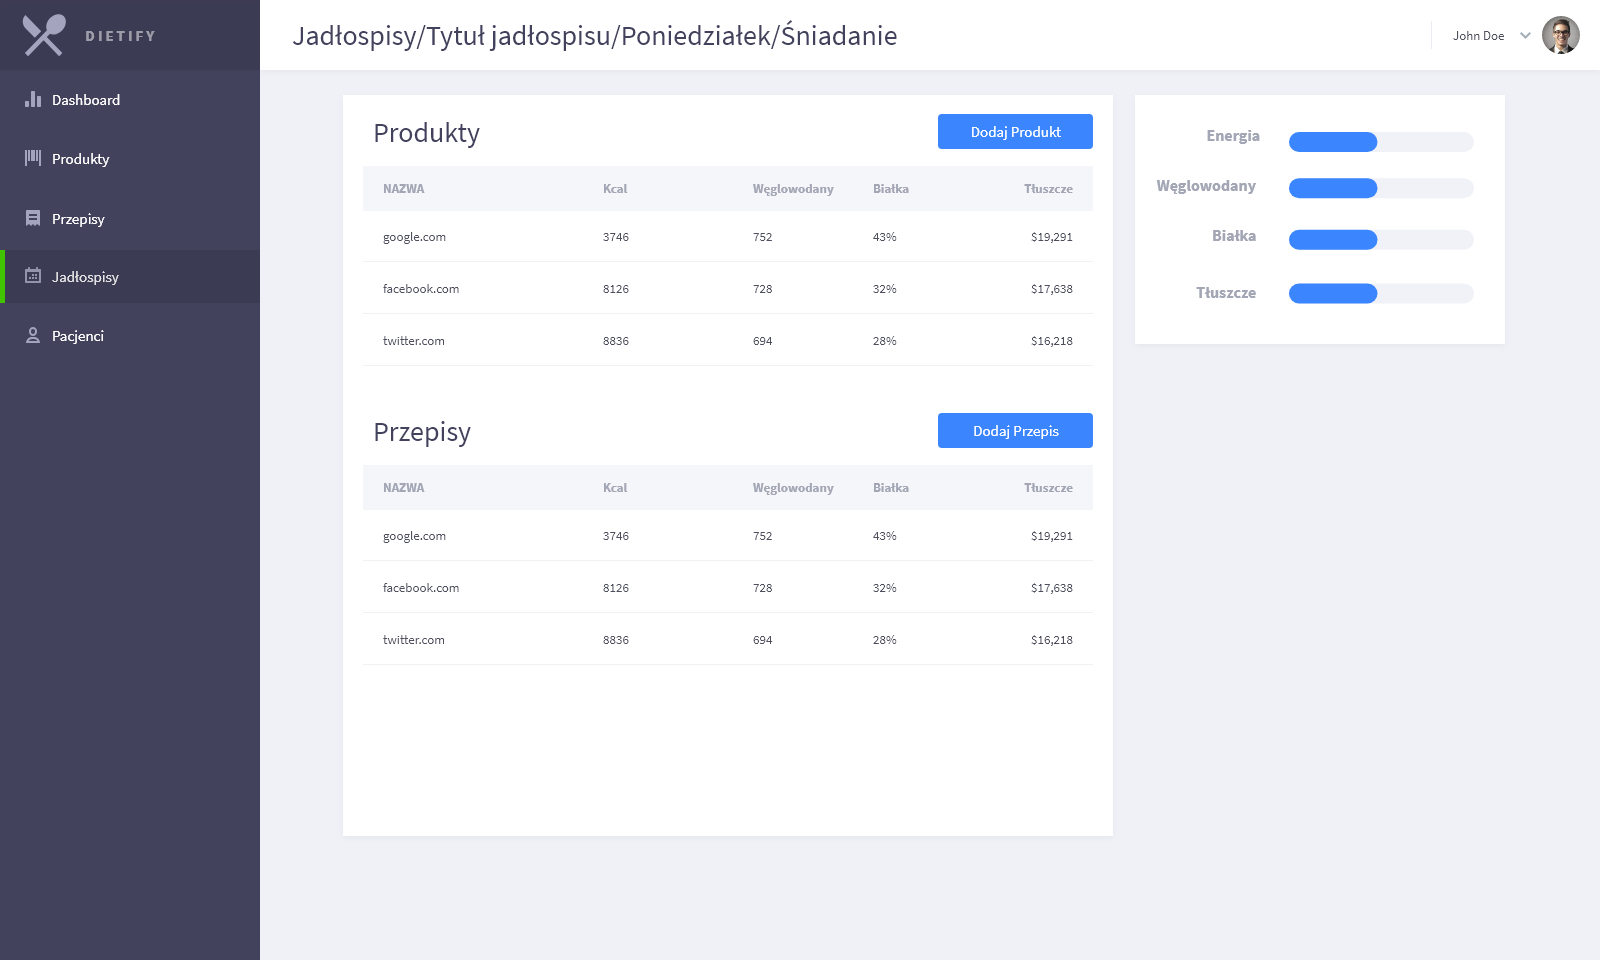
\includegraphics[width=0.9\textwidth]{img/mockups/mockup10.png}
        \caption{Mockup10 (opr.w).}\label{rysunek:mockup10}
    \end{figure}
\end{minipage}

\begin{minipage}{\textwidth}
    \begin{figure}[H]
        \centering\includegraphics[width=0.9\textwidth]{img/mockups/mockup11.png}
        \caption{Mockup11 (opr.w).}\label{rysunek:mockup11}
    \end{figure}
\end{minipage}

\begin{minipage}{\textwidth}
    \begin{figure}[H]
        \centering\includegraphics[width=0.9\textwidth]{img/mockups/mockup12.png}
        \caption{Mockup12 (opr.w).}\label{rysunek:mockup12}
    \end{figure}
\end{minipage}

\begin{minipage}{\textwidth}
    \begin{figure}[H]
        \centering\includegraphics[width=0.9\textwidth]{img/mockups/mockup13.png}
        \caption{Mockup13 (opr.w).}\label{rysunek:mockup13}
    \end{figure}
\end{minipage}

\begin{minipage}{\textwidth}
    \begin{figure}[H]
        \centering\includegraphics[width=0.9\textwidth]{img/mockups/mockup14.png}
        \caption{Mockup14 (opr.w).}\label{rysunek:mockup14}
    \end{figure}
\end{minipage}

\begin{minipage}{\textwidth}
    \begin{figure}[H]
        \centering\includegraphics[width=0.9\textwidth]{img/mockups/mockup15.png}
        \caption{Mockup15 (opr.w).}\label{rysunek:mockup15}
    \end{figure}
\end{minipage}

\begin{minipage}{\textwidth}
    \begin{figure}[H]
        \centering\includegraphics[width=0.9\textwidth]{img/mockups/mockup16.png}
        \caption{Mockup16 (opr.w).}\label{rysunek:mockup16}
    \end{figure}
\end{minipage}

\section{Model bazy danych}

\begin{minipage}{\textwidth}
    \begin{figure}[H]
        \centering\includegraphics[width=0.9\textwidth]{img/class-diagrams/produkty.png}
        \caption{Produkty (opr.w).}\label{rysunek:produkty}
    \end{figure}
\end{minipage}

\begin{minipage}{\textwidth}
    \begin{figure}[H]
        \centering\includegraphics[width=0.9\textwidth]{img/class-diagrams/przepisy.png}
        \caption{Przepisy (opr.w).}\label{rysunek:przepisy}
    \end{figure}
\end{minipage}

\begin{minipage}{\textwidth}
    \begin{figure}[H]
        \centering\includegraphics[width=0.9\textwidth]{img/class-diagrams/jadospisy.png}
        \caption{Jadłospisy (opr.w).}\label{rysunek:jadlospisy}
    \end{figure}
\end{minipage}

\begin{minipage}{\textwidth}
    \begin{figure}[H]
        \centering\includegraphics[width=0.9\textwidth]{img/class-diagrams/wizyty.png}
        \caption{Wizyty (opr.w).}\label{rysunek:wizyty}
    \end{figure}
\end{minipage}

\thispagestyle{normal}

    \chapter{Implementacja}
\section{Wykorzystywane środowiska i narzędzia programistyczne}
\section{Instalacja oprogramowania}
\subsection{Wymagania wstępne}
\begin{itemize}
    \item Java 8 \cite{java}
    \item Node.js 10 \cite{nodejs}
    \item Docker + Docker Compose
\end{itemize}
\section{Instrukcja użytkowania}

\thispagestyle{normal}

    \chapter{Testy}
\section{Testy jednostkowe}
\section{Testy integracyjne}
\section{Testy akceptacyjne}

    %% !TeX program = latexmk
% !TeX spellcheck = pl_PL
% !TeX root = example.tex

\chapter{Jak korzystać z szablonu pracy}

Klasa przygotowana jest zgodnie z zaleceniami dostępnymi ze strony \url{} i może być wykorzystana do składu pracy \textbf{inżynierskiej} lub \textbf{magisterskiej} na wydziale mechanicznym.

Klasa zgodnie z \href{http://www.wmech.pwr.wroc.pl/88428.dhtml}{wymaganiami Wydziału Mechanicznego} składa stronę tytułową i~stosuje się do zaleceń (czcionka, zasady numeracji, odstępy,\ldots).

Po raz pierwszy w roku akademickim 2015/2016 prace dyplomowe będą sprawdzane przez program antyplagiatowy. Nie wiadomo jeszcze jakie to będzie miało konsekwencje dla prac składanych w LaTeXu. Proponuję zaglądać do \href{http://kmim.wm.pwr.edu.pl/myszka/tag/antyplagiat/}{aktualności temu poświęconych}.

\section{Użycie}

\begin{enumerate}
\item
Praca magisterska i inżynierska.

Wychodzi, że tak na prawdę powinny być dwie wersje pracy: do archiwum (marginesy 2,5 cm) i „dla promotora”\footnote{Ciekawe po co mu…?}. Wersja dla promotora powinna mieć trochę większy margines od strony oprawy (35mm), najprawdopodobniej będzie drukowana \textbf{jednostronnie} i, żeby była łatwiejsza do czytania będzie złożona z interlinią \textbf{1,5}.

Jak tak to tak:  pojawiły się dwie dodatkowe opcje klasy:
\begin{enumerate}
\item
\texttt{archiwum}: \verb|\usepackage[magister,archiwum]{dyplom}| — wersja do archiwum
\item
\texttt{druk}: \verb|\usepackage[inzynier,druk]{dyplom}| — wersja do „druku” (i oprawy).
\end{enumerate}
\textbf{W przypadku braku opcji — wybierana jest wersja do archiwum!}

Tak na prawdę, to w przypdku braku opcji powinna być wybierana wersja druk. Wybrałem jednak opisane wyzej zachowanie, aby zachowanie zmodyfikowanej klasy było zgodne z dotychczasowym. Zalecam przeprowadzanie redakcji tekstu w trybie druku i pozostawienie dokumentu „jak wyjdzie” w trybie archiwum. Chyba, że ilustracje będą zachowywać się bardzo dziwnie…

Ponieważ „doszły do mnie” jakieś dziwne informacje, że ze stroną tytułową jest coś nie tak, dokonałem kolejnych porównań. Różnica jest jedna: obecność ramki wokół tytułów pracy. W związku z tym, ramka została zlikwidowana. Można ją odzyskać dodając dodatkowy parametr: \verb|\usepackage[inzynier,druk,ramka]{dyplom}| i~się pojawi…
\item
Praca magisterska:
\begin{verbatim}
\documentclass[magister]{dyplom}
\end{verbatim}
Dodatkowo zdefiniować należy sposób kodowania polskich liter. W przypadku systemu Windows będzie to najprawdopodobniej:
\begin{verbatim}
\usepackage[cp1250]{inputenc}
\end{verbatim}
a w przypadku systemów linuksowych:
\begin{verbatim}
\usepackage[utf8]{inputenc}
\end{verbatim}

Dodatkowo zdefiniować należy „metadane”:
\begin{itemize}
\item
Nazwisko autora:
\begin{verbatim}
\author{Imię Nazwisko}
\end{verbatim}
\item
Tytuł pracy (w języku polskim):
\begin{verbatim}
\title{Tytuł Pracy}
\end{verbatim}
\item
Tytuł pracy po angielsku
\begin{verbatim}
\titlen{Work Title}
\end{verbatim}
\item
Nazwisko promotora
\begin{verbatim}
\promotor{prof. dr hab. inż. Imię Nazwisko, prof. PWr.}
\end{verbatim}
\item
Kierunek
\begin{verbatim}
\kierunek{Prawo}
\end{verbatim}
\item
Specjalność:
\begin{verbatim}
\specjalnosc{Lewo}
\end{verbatim}
\item
W razię potrzeby wpisać można inną nazwę wydziału. Gdy nie zostanie wpisana — będzie tam Wydział Mechaniczny.
\begin{verbatim}
\wydzial{Wydział Elektryczny}
\end{verbatim}
\item
Praca może mieć konsultanta/konsultantów. Dodałem więc pole konsultant:
\begin{verbatim}
\konsultant{dr inż. Kazimierz Kabacki}
\end{verbatim}
Nazwisko konsultanta pojawi się miedzy nazwiskiem promotora a oceną. Pozostaje kwestia czy powinien to być „konsultant” czy raczej „konsulktanci”?
\end{itemize}
Powyższe metadane umieszczamy przed \verb|\begin{document}|:
\begin{verbatim}
\documentclass[magister]{dyplom}
\usepackage[utf8]{inputenc}

\author{Jan A. Backi}
\title{Lorem ipsum dolor sit amet, consectetuer adipiscing elit}
\titlen{Lorem ipsum dolor sit amet, consectetuer adipiscing elit}
\promotor{dr hab. inż. Jerzy Babacki, prof. nadzw. PWr., I-77}
\wydzial{Wydział Mechaniczny}
\kierunek{Prawo}
\specjalnosc{Lewo}

\begin{document}
\end{verbatim}
\item
Praca inżynierska:
\begin{verbatim}
\documentclass[inzynier]{dyplom}
\end{verbatim}
Dodatkowo zdefiniować należy sposób kodowania polskich liter. W przypadku systemu Windows będzie to najprawdopodobniej:
\begin{verbatim}
\usepackage[cp1250]{inputenc}
\end{verbatim}
a w przypadku systemów linuksowych:
\begin{verbatim}
\usepackage[utf8]{inputenc}
\end{verbatim}

Dodatkowo zdefiniować należy „metadane”:
\begin{itemize}
\item
Nazwisko autora:
\begin{verbatim}
\author{Imię Nazwisko}
\end{verbatim}
\item
Tytuł pracy (w języku polskim):
\begin{verbatim}
\title{Tytuł Pracy}
\end{verbatim}
\item
Tytuł pracy po angielsku
\begin{verbatim}
\titlen{Work Title}
\end{verbatim}
\item
Nazwisko promotora
\begin{verbatim}
\promotor{prof. dr hab. inż. Imię Nazwisko, prof. PWr.}
\end{verbatim}
\item
Kierunek
\begin{verbatim}
\kierunek{Prawo}
\end{verbatim}
%\item
%Specjalność:
%\begin{verbatim}
%\specjalnosc{Lewo}
%\end{verbatim}
\item
W razię potrzeby wpisać można inną nazwę wydziału. Gdy nie zostanie wpisana — będzie tam Wydział Mechaniczny.
\begin{verbatim}
\wydzial{Wydział Elektryczny}
\end{verbatim}
\item
Praca może mieć konsultanta/konsultantów. Dodałem więc pole konsultant:
\begin{verbatim}
\konsultant{dr inż. Kazimierz Kabacki}
\end{verbatim}
Nazwisko konsultanta pojawi się miedzy nazwiskiem promotora a oceną. Pozostaje kwestia czy powinien to być „konsultant” czy raczej „konsultanci”?

\end{itemize}
Powyższe metadane umieszczamy przed \verb|\begin{document}|:
\begin{verbatim}
\documentclass[magister]{dyplom}
\usepackage[utf8]{inputenc}

\author{Jan A. Backi}
\title{Lorem ipsum dolor sit amet, consectetuer adipiscing elit}
\titlen{Lorem ipsum dolor sit amet, consectetuer adipiscing elit}
\promotor{dr hab. inż. Jerzy Babacki, prof. nadzw. PWr., I-77}
\wydzial{Wydział Mechaniczny}
\kierunek{Prawo}
\specjalnosc{Lewo}

\begin{document}
\end{verbatim}

\end{enumerate}

\section{Dodatkowe zasoby}

Warto wspomnieć  o innych inicjatywach przyswojenia LaTeX{}a piszącym prace dyplomowe. Najważniejsza z nich to książka Tomasza Przechlewskiego \cite{tp-11-latex} oraz przygotowana przez niego klasa znajdująca się w \url{https://github.com/hrpunio/wzmgr}. Przykłady z książki znaleźć można w \url{https://github.com/hrpunio/pmdzpl}.


\section{Gdzie znaleźć?}

Pakiet można znaleźć pod adresem: \url{http://www.immt.pwr.wroc.pl/~myszka/dydaktyka/}. Wersja zarchiwizowana: \href{http://www.immt.pwr.wroc.pl/~myszka/TeX/dyplom/dyplom.zip}{dyplom.zip}

\section{Uwagi}

Wszelkie uwagi i postulaty należy kierować na adres Wojciech.Myszka@pwr.wroc.pl

W miarę potrzeby mogę szablon dostosować do wymagań innych wydziałow Politechniki Wrocławskiej.

\thispagestyle{normal}
    %\chapter{Ala ma kota}

ĄĆĘŁŃÓŚŹŻ ąćęłńóśźż\footnote{Przykład użycia polskich znaków diakrytycznych oraz przypisu w miejscu}. \lipsum[1]

\section{Odniesienie do pozycji z literatury (strona WWW)}

% Odniesienie do rysunku i cytowanie dokumentu. Dokumenty są definiowane w pliku literatura.bib
Reszta dokumentacji znajduje się w \cite{docker_compose_reference}. \lipsum[3]

\section{Odniesienie do książki}

Jak pisze Harel w \cite{harel_rzecz_2008}: \lipsum[7]

\section{Rysunek}

% Rysunek
\begin{figure}
\centering\includegraphics[width=.6\textwidth]{img/swarm-network}
\caption{Docker ma sieć \cite{docker_compose_reference}.}  \label{rys:network}% Źródło rysunku i etykieta przez którą odwołujemy się do rysunku.
\end{figure}

Jak widać na rys. \ref{rys:network} Docker ma wewnętrzną sieć. \lipsum[1]


\subsection{Rysunek z kotem}

Jak widać na rys.\ref{rysunek:kot} Ala ma kota. \lipsum[9-10] 

\begin{figure}[h!]
\centering\includegraphics[width=.4\textwidth]{img/kotek}
\caption{Ala ma kota (opr.wł).}\label{rysunek:kot}
\end{figure}

\subsection{Tabela}

Co uwzględniono w tabeli \ref{tabela:coktoma}. \lipsum[13-15] 

% Tabela. Nazwa tabeli u góry.
\begin{table}[h!]
\centering\caption{Co kto ma \cite{harel_rzecz_2008} (patrz też dodatek~\ref{Dod1}) \label{tabela:coktoma}}
\begin{tabular}{|l|l|l|}% wyrównanie kolumn tabeli -> l c r - do lewej, środka, do prawej
\hline
Ala & ma & kota \\
\hline
Ola & ma & psa \\
\hline
Ula & ma & małpę\\
\hline
\end{tabular}
\end{table}

\lipsum[19-20] Warto wspomnieć, że w \cite{aizawa_groundwater_2009} rzecz przedstawiona jest zupełnie inaczej. Poniższy wzór:

\begin{equation}
\sum_{i=1}^{\infty}a_i
\label{eq:mojWzor}
\end{equation}

Wzór \ref{eq:mojWzor} wskazuje że dowód podany w \cite{kaleta_experimental_2005} może zostać podważony. \lipsum[9]

\section{Kod źródłowy}

% lub {java} albo {bash} albo {text}
\begin{listing}[h!]
\begin{minted}{c} 
int main()
{
   int a=2*3;
   printf("**Ala ma kota\n**");
   while(!I2C_CheckEvent(I2C1, I2C_EVENT_MASTER_MODE_SELECT)); /* EV5 */
   return 0;
}
\end{minted}
\caption{Przykładowy algorytm w języku C (opr. wł.)} \label{listing:moj}
\end{listing}

W moim kodzie \ref{listing:moj} zrobiłem coś wspaniałego. \lipsum[4]

\begin{table}[h]
	\begin{tabularx}{\textwidth}{|>{\setlength\hsize{1.4\hsize}\setlength\linewidth{\hsize}}X|>{\setlength\hsize{.9\hsize}\setlength\linewidth{\hsize}}X|>{\setlength\hsize{.7\hsize}\setlength\linewidth{\hsize}}X|}
		\hline
		\multicolumn{3}{|c|}{Classification of the criticel point $(0,0)$ of $x'=Ax,|\mathbf{A}|\not=0$.}\\
		\hline
		Types & Type of Critical Point & Stability \\
		\hline
		1. Real unequal eigenvalues of same sign
		\begin{itemize}
			\item $\lambda_1 > \lambda_2 > 0$
			\item $\lambda_1 < \lambda_2 < 0$
		\end{itemize} &
		\vphantom{1. Real unequal eigenvalues of same sign}
		\begin{itemize}
			\item Improper Node/Node
			\item Improper Node/Node
		\end{itemize} &
		\vphantom{1. Real unequal eigenvalues of same sign}
		\begin{itemize}
			\item Unstable
			\item Asym. Stable
		\end{itemize}\\
		\hline
		2. Real unequal eigenvalues of opposite sign
		\begin{itemize}
			\item $\lambda_2 < 0 >\lambda_1$
		\end{itemize} &
		\vphantom{2. Real unequal eigenvalues of opposite sign}
		\begin{itemize}
			\item Saddle Point
		\end{itemize} &
		\vphantom{2. Real unequal eigenvalues of opposite sign}
		\begin{itemize}
			\item Unstable
		\end{itemize}\\
		\hline
		3. Equal eigenvalues \newline Subtype 1: Two Independent vectors
		\begin{itemize}
			\item $\lambda_1 = \lambda_2 > 0$
			\item $\lambda_1 = \lambda_2 < 0$
		\end{itemize} &
		\vphantom{3. Equal eigenvalues} \vphantom{ Subtype 1: Two Independent vectors}
		\begin{itemize}
			\item Proper Node
			\item Proper Node
		\end{itemize} &
		\vphantom{3. Equal eigenvalues} \vphantom{ Subtype 1: Two Independent vectors}
		\begin{itemize}
			\item Unstable
			\item Asym. Stable
		\end{itemize}\\
		\hline
	\end{tabularx}
\end{table}
\thispagestyle{normal}

    \chapter*{Zakończenie}

W pracy udało mi się dużo zrobić. \lipsum[17]

Mnóstwo innych rzeczy da się poprawić i rozwinąć. \lipsum[23]
\thispagestyle{normal}

    % W pracy pojawią się tylko prace naprawdę cytowane.
    % \nocite{*}

    \bibliography{literatura}
    \bibliographystyle{dyplom}

    \listoffigures
    \listoftables
    \listof{listing}{Spis kodów źródłowych}

    % \appendixpage
% \addappheadtotoc

\appendix
\begin{appendices}
\chapter{To powinien być dodatek}\label{Dod1}
\lipsum[9-11]
\end{appendices}

\end{document}
